% Chapter Template 
% cSpell: words Mininet prototipado parencite enrutamiento includegraphics veth  mininetonf cellcolor Nicira vswitchd interconectar multicapa datapath ovsflow resizebox flowtable netlink OVSDB dpctl ofctl vsctl rowcolor mininetovs

\chapter{Desarrollo} % Main chapter title

\label{Chapter3} % Change X to a consecutive number; for referencing this chapter elsewhere, use \ref{ChapterX}

%----------------------------------------------------------------------------------------
%	SECTION 1
%----------------------------------------------------------------------------------------

\section{Desarrollo de la investigación}

En la presente sección se busca explicar brevemente cómo se fue estructurando y desarrollando el algoritmo en cuestión. 

Las redes implementadas en esta investigación fueron redes del tipo $S^3PR$ dado que modelan la ejecución concurrente de procesos de trabajo. La finalización de alguno de estos puede iniciar más de una nueva operación. Como resultado de estas características dinámicas, pueden ocurrir dos situaciones: conflicto y deadlock. 

El conflicto puede ocurrir cuando dos o más procesos requieren un recurso común al mismo tiempo. Por ejemplo, dos estaciones de trabajo pueden compartir un sistema de transporte común o necesitar acceso al mismo almacenamiento. Una forma sencilla de resolver el conflicto es asignar un nivel de prioridad a cada uno de los procesos. 

El deadlock puede suceder al compartir dos recursos entre los dos procesos. En este caso, se puede alcanzar un estado en el que ninguno de los procesos puede continuar. Tenga en cuenta que uno de los procesos puede continuar si el conflicto se puede resolver, mientras que en el caso de deadlock no se puede hacer nada para que el sistema vuelva a funcionar.


%----------------------------------------------------------------------------------------
%	SECTION Modelo de Desarrollo
%----------------------------------------------------------------------------------------
\section{Modelo de desarrollo}
Para la elaboración del presente proyecto se optó por utilizar un modelo iterativo e incremental. A grandes rasgos, este tipo de modelo de desarrollo no es más que un conjunto de tareas agrupadas en pequeñas etapas repetitivas, las cuales inician con un análisis y finalizan con una versión nueva del algoritmo y sus conclusiones. \\

\par Se planifica un proyecto en distintos bloques temporales denominados iteraciones. Dentro de una iteración se repite un determinado proceso de trabajo sobre uno o varios objetivos, obteniéndose al final de la misma un resultado con más funcionalidades implementadas que el de la iteración anterior. La ventaja principal de este modelo es que no se debe esperar a que el sistema esté completo para que el mismo sea utilizable y operacional. \\

\par Para lograr esto, al realizar el análisis de una iteración, se especifican los objetivos que se esperan conseguir al finalizar la misma. Estos se establecen en función de los requerimientos, de los riesgos y de la evaluación de los resultados de las iteraciones precedentes. Se busca que en cada iteración los componentes logren evolucionar el producto dependiendo de aquellos completados en las iteraciones antecesoras. \\

\par \noindent La implementación del algoritmo se realizó en cuatro iteraciones:
\begin{itemize}
    \item \textbf{Iteración 1}: Procesamiento de los archivos '.html' y detección de estados de deadlock.
    \begin{enumerate}
        \item Realizar la conversión de los archivos de formato '.html' exportados del Petrinator y su posterior procesamiento para que sean utilizados como entradas en el algoritmo.
        \item Detección de estados de deadlock basándose en los fundamentos teóricos (Capítulo \ref{Chapter2}).
        \item Una vez detectado, se evita alcanzar el mismo inhibiendo el disparo de la transición que lo desencadena.
    \end{enumerate}
    
    \item \textbf{Iteración 2}: Sifones en estado de deadlock y plaza de control.
    \begin{enumerate}
        \item Detectar los sifones vacíos en estado de deadlock.  
        \item Obtener el marcado inicial de cada sifón.
        \item Detectar la transición cuyo disparo lleva al camino del deadlock.
        \item Incorporar plaza y arco de control (salida) que evite el vaciado del sifón en cuestión.
    \end{enumerate}
    
    \item \textbf{Iteración 3}: Sifones mínimos en estado de deadlock y supervisor.
    \begin{enumerate}
        \item Obtener los sifones mínimos vacíos (bad siphons) en estado de deadlock.
        \item Determinar el marcado y arcos (entrada y salida) del supervisor.
        \item Incorporar los supervisores que eviten el vaciado de los sifones en cuestión.
    \end{enumerate}
    
    \item \textbf{Iteración 4}: Mantener los T-invariantes e interfaz de salida hacia el Petrinator
    \begin{enumerate}
        \item Realizar el análisis sobre la totalidad de la red permitiendo preservar los T-invariantes de la red original.
        \item Modificar el archivo de extensión '.pflow' de la red en cuestión, para agregar plazas, arcos y quitar estos últimos en caso de ser necesario.
    \end{enumerate}
\end{itemize}

\par \noindent Las mismas serán tratadas con mayor profundidad a lo largo de este capitulo. 
%----------------------------------------------------------------------------------------
%	SECTION 3
%----------------------------------------------------------------------------------------

\section{Iteración 1: Algoritmo v1.0}
\subsection{Introducción}
En esta iteración se hizo foco en analizar el grafo de alcanzabilidad de las redes, detectando los estados de deadlock alcanzables y trazando las secuencias de disparo que desencadenan a los mismos. 
\subsection{Objetivos}
\begin{itemize}
	\item Conversión de archivos de formato '.html' (salida del software Petrinator) a archivos tipo '.txt' para facilitar la lectura de los datos en el algoritmo.
	\item Detectar el/los estado/s con deadlock y evitar el camino que desencadenan a ellos.
\end{itemize}

\subsection{Desarrollo}
\subsubsection{Herramienta a utilizar}
El software seleccionado para obtener la información necesaria para el desarrollo del algoritmo fue Petrinator \cite{petrinator} debido a que el mismo fue desarrollado dentro del Laboratorio de Arquitecturas de Computadoras (LAC) lo que nos permitió solicitar modificaciones según nuestras necesidades. 

\noindent Sus principales características son:
\begin{itemize}
	\item Una interfaz intuitiva que permite la creación, edición, almacenamiento y exportación de redes de Petri.
	\item Código abierto y bajo licencia GPL. 
\end{itemize}

\paragraph{Datos necesarios}
Se utilizaron las funcionalidades del Petrinator para obtener y exportar la siguiente información de la red:
\begin{itemize}
    \item Análisis de Invariantes (Invariant analysis)
    \begin{itemize}
        \item T-invariantes
        \item P-invariantes
    \end{itemize}
    \item Matrices
    \begin{itemize}
        \item Pre(+)
        \item Post(-)
    \end{itemize}
    \item Sifones y Trampas (Siphons and Traps)
    \begin{itemize}
        \item Sifones (plazas que lo componen)
        \item Trampas (plazas que lo componen)
    \end{itemize}
    \item Grafo de Alcanzabilidad (Reachability graph)
    \begin{itemize}
        \item Estados en deadlock
        \item Marcado inicial de los sifones
    \end{itemize}
\end{itemize}

\subsubsection{Conversión de datos}

Como puente entre el software Petrinator y el algoritmo principal, se desarrolló un algoritmo de conversión en Python “html\_to\_txt”, el cual dados los archivos '.html' exportados por el software trabaja sobre estos, con el fin de obtener los datos característicos de la red (mencionados anteriormente) en el formato adecuado de entrada que alimentará al algoritmo en desarrollo, en este caso matrices y vectores.

\subsubsection{Construcción del algoritmo}

Una vez realizada la carga y el filtrado de los datos exportados del software Petrinator, se llevó a cabo la detección de todos los estados con deadlock presentes en la red. Luego, se selecciona uno de estos y se trazan las secuencias de disparo que desencadenaron al mismo, se verifican todos los arcos de los estados que desencadenaron al mismo; si alguno de estos estados también estaban en deadlock se inhiben los mismos en el vector de sensibilización, esto se realiza recursivamente hasta encontrar algún estado que no presente deadlock dejando \textbf{solamente} este brazo habilitado en el vector de sensibilización, de esta manera nos aseguramos de no entrar en un camino que solo conduce al estado de deadlock.
\bigskip

\begin{figure}[H]
	\centering
	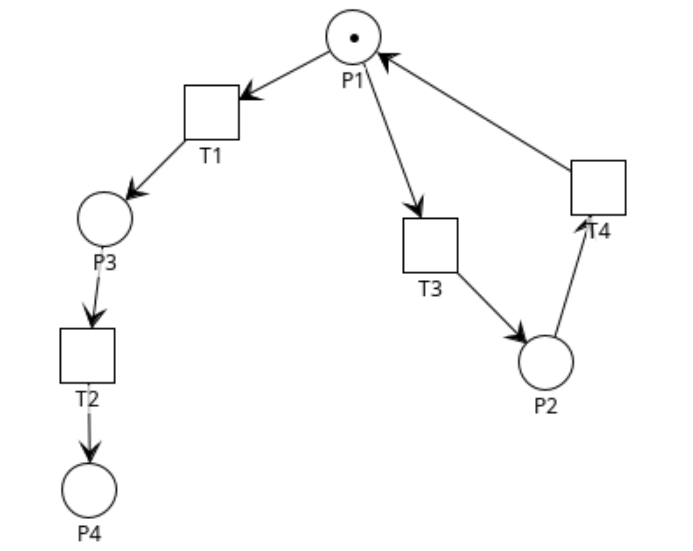
\includegraphics[scale=0.50]{Figures/algoritmo1/1.png}
	\caption{RdP con un estado de deadlock.}
	\label{fig:rdp3.1}
  \end{figure}

La red que se observa en la figura \ref{fig:rdp3.1} presenta 4 estados alcanzables y uno de ellos es un estado con deadlock.
\begin{itemize}
	\item $S_0[1,0,0,0]$
	\item $S_1[0,0,1,0]$
	\item \textcolor{red}{$S_2[0,0,0,1]$}
	\item $S_3[0,1,0,0]$
\end{itemize}
\bigskip

Como se mencionó con anterioridad, se parte desde el estado $S_2$ verificando que estado nos lleva al mismo. El único estado que nos lleva a este es el $S_1$ (al ejecutarse la transición $T_2$) por este motivo se inhibe esta transición del vector de sensibilizadas. Al realizar esto ahora el estado $S_1$ se convierte en un estado con deadlock, y se realiza el mismo procedimiento mencionado con anterioridad inhibiendo la transición $T_1$ que es la única que nos lleva a este estado a partir del estado $S_0$. 
De esta manera se obtiene una red sin deadlock dado que nunca se va tomar el camino de la izquierda,ya que se produjo la inanición de esta parte de la red.

\bigskip
Posteriormente se decidió aplicar la misma hipótesis sobre una red más compleja, con un mayor número de estados en su grafo de alcanzabilidad. Para esto se eligió la red representada en la figura \ref{fig:panama}

\begin{figure}[H]
	\centering
    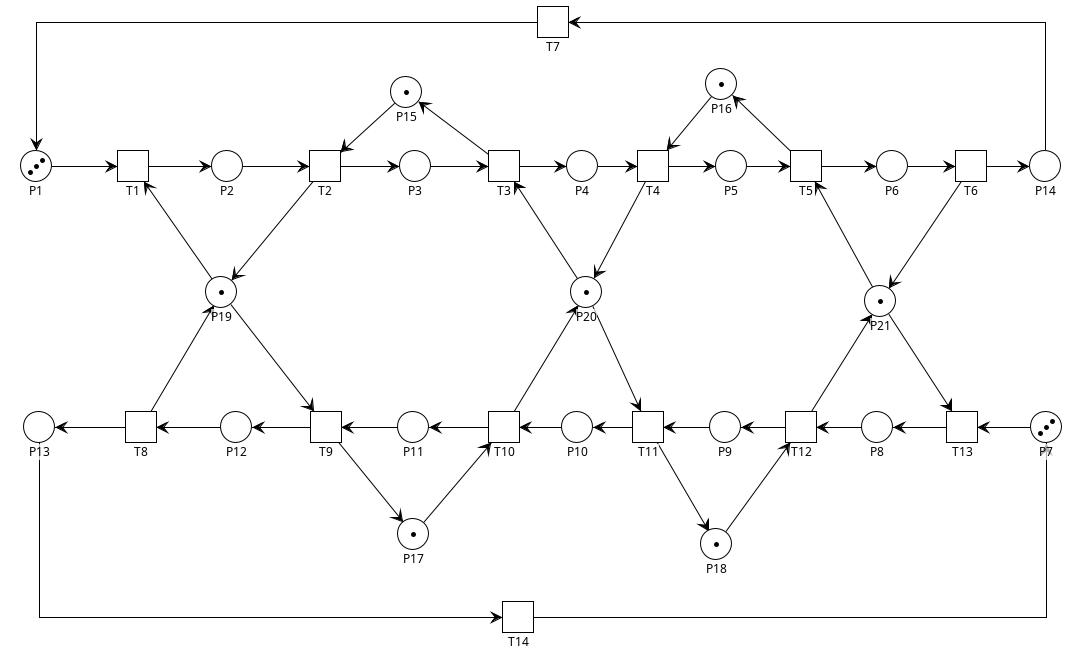
\includegraphics[width=\textwidth]{Figures/algoritmo1/panama.png}
    \caption[RdP Canal de Panamá.]{RdP Canal de Panamá. \footnotemark}
	\label{fig:panama}
 \end{figure} \footnotetext{Figura adaptada del libro \textit{An  Algorithm  for  Deadlock Prevention  Based  on  Iterative  Siphon  Control  of  Petri  Net} \cite{paperpanama} .}

\begin{figure} [H]
	\centering
	\subfloat [Estado número 82.] {
	    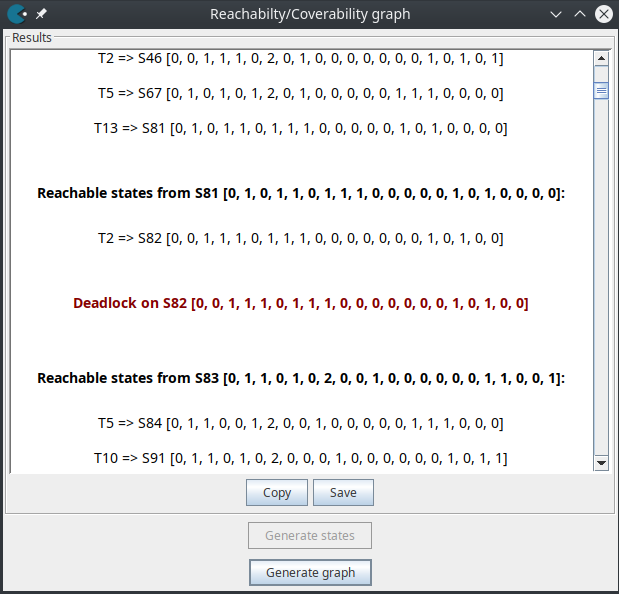
\includegraphics[scale=0.45]{Figures/algoritmo1/version1_deadlock2.png}
    	\label{fig:state_deadlock1}
    }
    \subfloat [Estado número 484.] {
        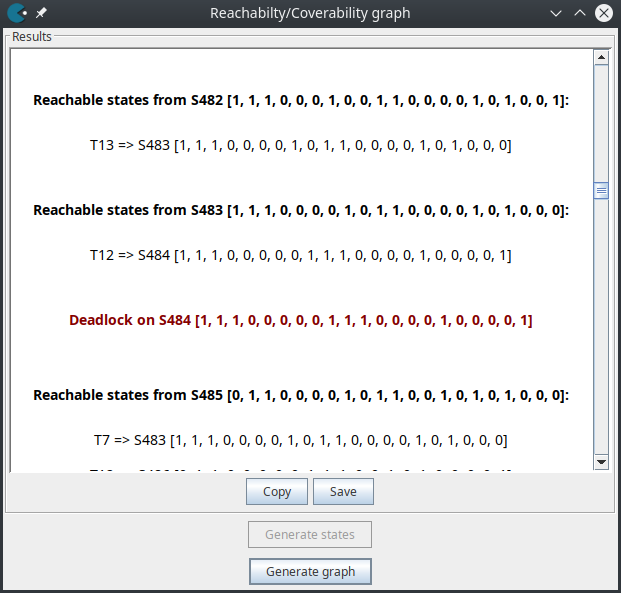
\includegraphics[scale=0.45]{Figures/algoritmo1/version1_deadlock.png}
    	\label{fig:state_deadlock2}
    } 
   \caption{Estados de deadlock.} 
\end{figure}

Como se puede observar en las figuras \ref{fig:state_deadlock1} y \ref{fig:state_deadlock2} donde las transiciones $T_2$ y $T_{12}$ al ser ejecutadas llevan a los estados de deadlock; al deshabilitar la ejecución de las mismas la red sólo permite dos disparos (de las transiciones $T_1$ y $T_{13}$), luego de estos la red no se vuelve a ejecutar.
Esta solución no es viable dado que la solución alcanzada al inhibir estas transiciones no representa la ejecución del modelo original.

\subsection{Conclusiones}
Si bien se alcanzó el objetivo planteado, este primer algoritmo no era escalable dado que si bien lograba resolver el deadlock para redes simples, en el caso de redes más complejas no llegaba a converger a una solución. 
Sin embargo, gran parte de las funcionalidades implementadas fueron utilizadas en las posteriores versiones del mismo.
\bigskip

%----------------------------------------------------------------------------------------
%	SECTION 4
%----------------------------------------------------------------------------------------

\section{Iteración 2: Algoritmo v2.0}
\subsection{Introducción}
Al observar que la red presentaba un camino que llevaba al deadlock, se comenzó a analizar el porqué de este deadlock y observamos que el mismo se producía por el vaciado de al menos un sifón de la red. En esta nueva versión se hizo hincapié en evitar esta problemática.

\subsection{Objetivos}
\begin{itemize}
	\item Encontrar los sifones vacíos en estado de deadlock.
	\item Evitar estados con deadlock.
\end{itemize}

\subsection{Desarollo}
En cuanto a los datos necesarios para el funcionamiento del algoritmo se reutiliza el código que permite la conversión de los mismos implementado en la versión 1.0 del algoritmo. 
A diferencia de la versión anterior, en vez de inhibir el arco imposibilitando la ejecución del mismo lo que se hace es lo siguiente:
\begin{enumerate}
    \item Detectar el sifón vacío en el estado con deadlock.
    \item Obtener el marcado del mismo en el estado inicial.
    \item Detectar la transición cuyo disparo lleva a ese camino de deadlock.
    \item Colocar una plaza “de control” cuyo marcado es la marca del sifón menos uno, evitando de esta manera que el sifón se vacíe (dejando su marcado al menos con un token).
\end{enumerate}

\begin{figure}[H]
	\centering
	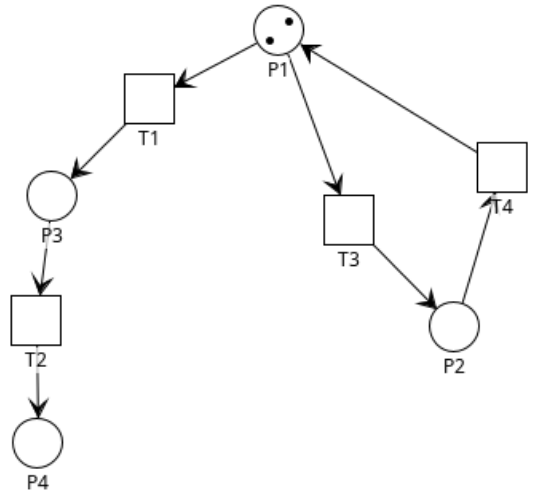
\includegraphics[scale=0.5]{Figures/algoritmo2/1.png}
	\caption{RdP con un estado de deadlock.}
	\label{fig:rdp3.2}
  \end{figure}

\begin{figure}[H]
	\centering
	\subfloat[Sifón]{
	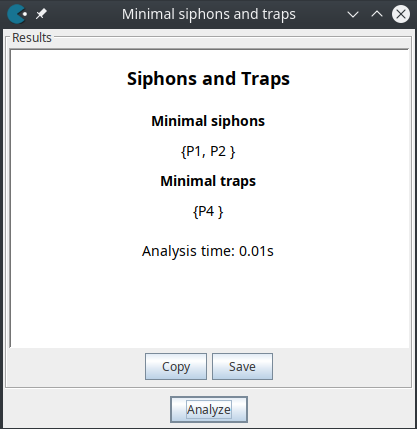
\includegraphics[scale=0.5]{Figures/algoritmo2/sifon.png}
	\label{fig:rdp3.2sifon}
	}
	\subfloat[Grafo de alcanzabilidad.]{
	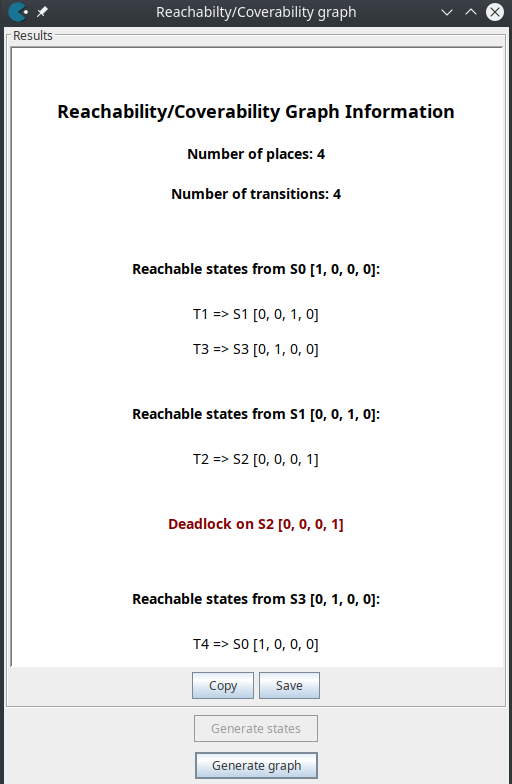
\includegraphics[scale=0.5]{Figures/algoritmo2/grafo.png}
	\label{fig:rdp3.2grafo}
	}
	\caption{Análisis de la figura \ref{fig:rdp3.2}.}
    \end{figure}


En la figura \ref{fig:rdp3.2} se puede observar que si la red ejecuta a la transición $T_1$ y luego $T_2$ dos veces, la red se bloquea. Como se puede observar en la figura \ref{fig:rdp3.2grafo} al ejecutar $T_2$ desde el estado $S_1$ conduce al deadlock. Al analizarla mediante el algoritmo y conociendo que el sifón que se presenta en la red está compuesto por $\{P_1,P_2\}$ como se ve en la figura \ref{fig:rdp3.2sifon} con un marcado inicial de 2, se obtiene un controlador que permite la ejecución de $T_1$ una única vez, es decir, una vez ejecutada ésta la parte izquierda de la red no se podrá volver a ejecutar.

\begin{figure}[H]
	\centering
	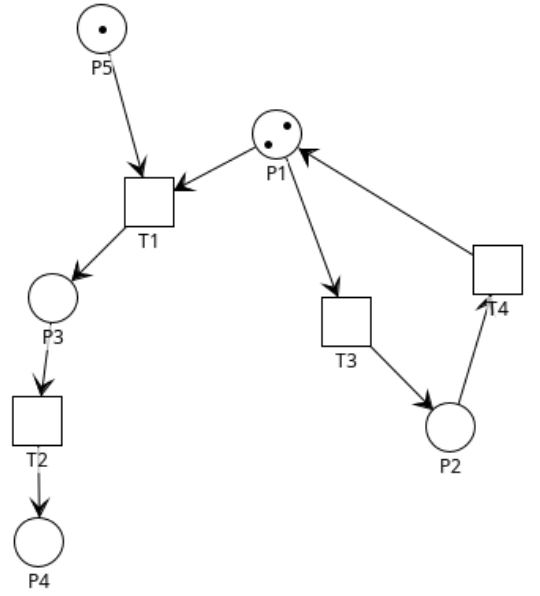
\includegraphics[scale=0.55]{Figures/algoritmo2/2.png}
	\caption{Control sobre la RdP.}
	\label{fig:rdp3.3}
  \end{figure}

\bigskip
Posteriormente se decidió aplicar la misma hipótesis sobre una red más compleja, con un mayor número de estados en su grafo de alcanzabilidad. Para esto se eligió la red representada en la figura \ref{fig:panama}

\begin{figure}[H]
	\centering
	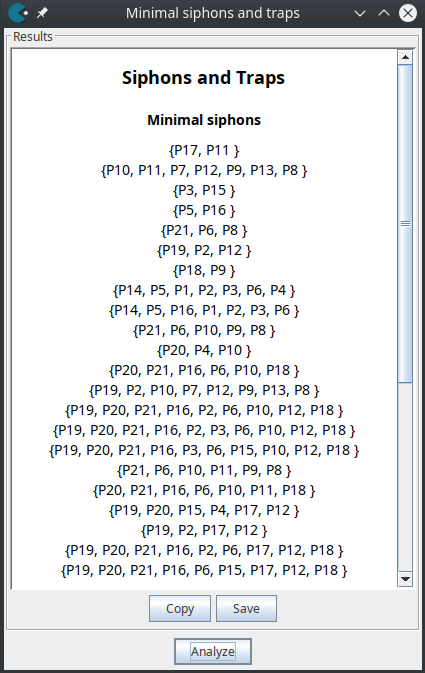
\includegraphics[scale=0.55]{Figures/algoritmo2/sifones_panama.png}
	\caption{Sifones RdP Panamá.}
	\label{fig:rdp_panama_sifones}
  \end{figure}

Como se puede observar en la figura \ref{fig:rdp_panama_sifones} estos son los sifones presentes en la red. Al obtener los estados con deadlock \ref{fig:state_deadlock1} y \ref{fig:state_deadlock2} se indagó para verificar cuáles eran los sifones vacíos en los mismos.
Para el estado número 82 el sifón que se vacía es el compuesto por las plazas \{$P_4, P_{12}, P_{15}, P_{17}, P_{19}, P_{20}$\} (\ref{fig:rdp_panama_sifon1}), mientras que para el estado número 484 el sifón vacío es el compuesto por las plazas \{$P_6, P_{10}, P_{16}, P_{18}, P_{20}, P_{21}$\} (\ref{fig:rdp_panama_sifon2}).

\begin{figure}[H]
	\centering
	\subfloat[Sifón izquierdo]{
	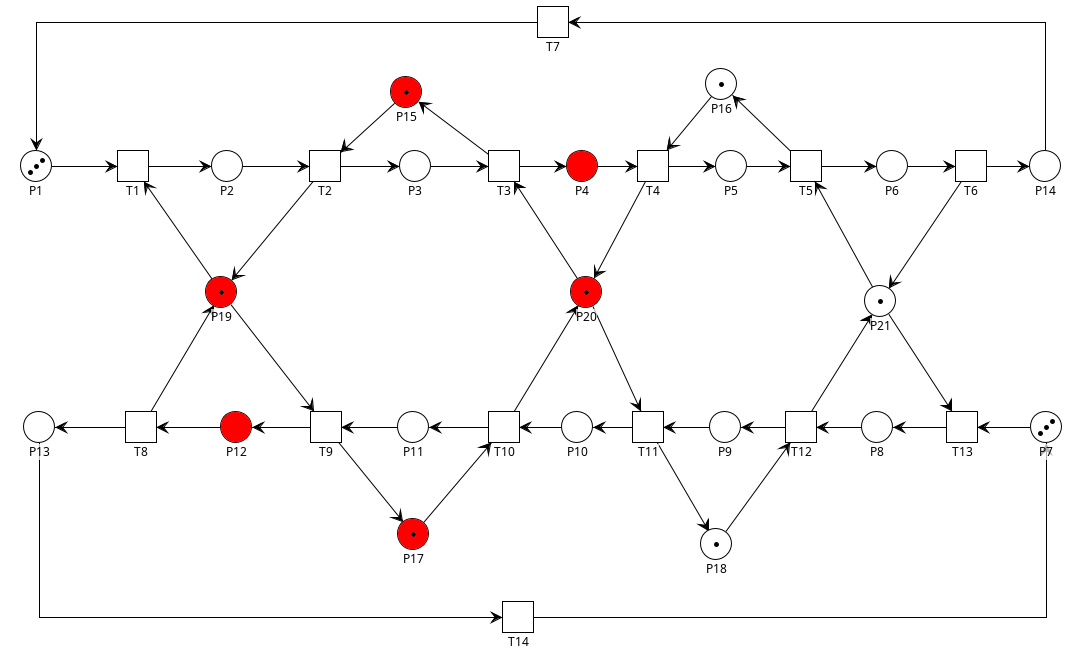
\includegraphics[width=\textwidth]{Figures/algoritmo2/panamaizq.png}
	\label{fig:rdp_panama_sifon1}
	}\\
    \subfloat[Sifón derecho]{
	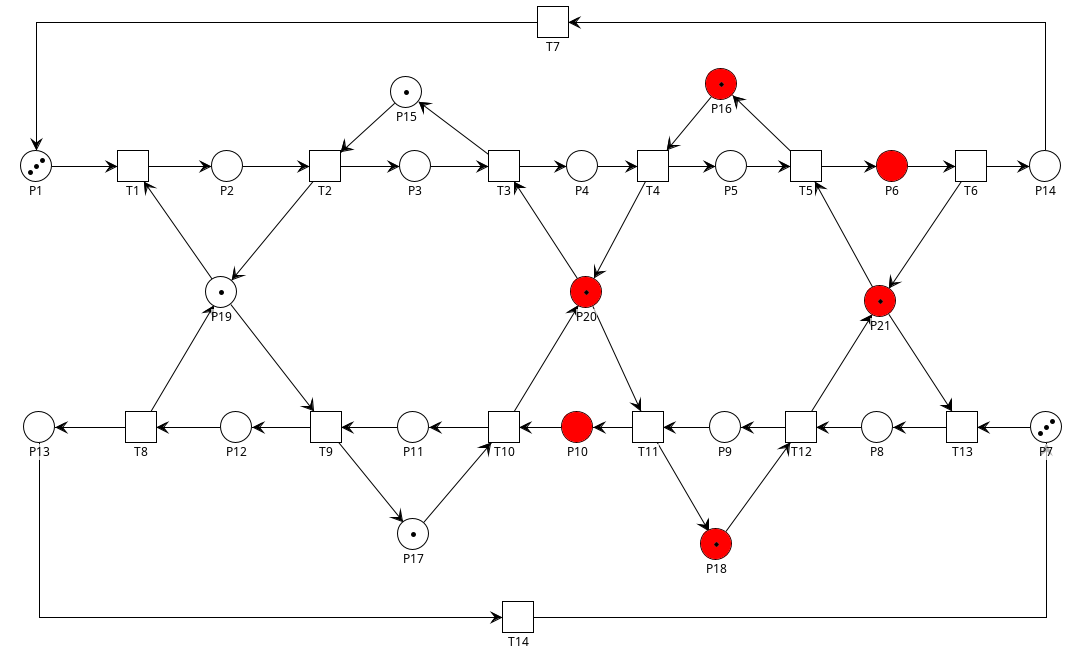
\includegraphics[width=\textwidth]{Figures/algoritmo2/panamader.png}
	\label{fig:rdp_panama_sifon2}
	}
	\caption{Sifones vacíos RdP Panamá}
\end{figure}

En las figuras \ref{fig:rdp_panama_sifon1} y \ref{fig:rdp_panama_sifon2} se pueden observar, destacados en color rojo, los sifones que se vacían en el estado de deadlock. De los mismos se obtiene el marcado inicial para luego colocar una plaza de control correspondiente a cada uno.

\begin{figure}[H]
	\centering
	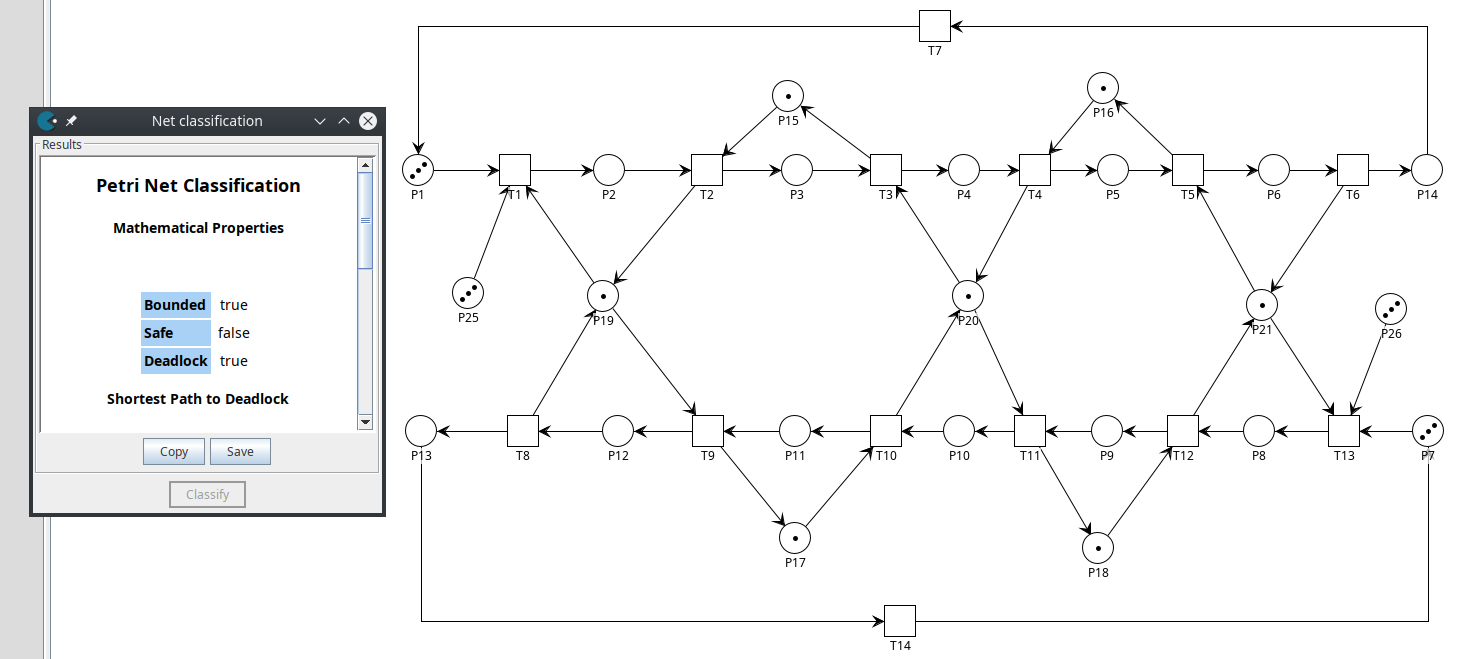
\includegraphics[width=\textwidth]{Figures/algoritmo2/panama_control_deadlock_true.png}
	\caption{Control RdP Panamá, deadlock true.}
	\label{fig:rdp_panama_deadlock_true}
  \end{figure}

\subsection{Conclusiones}
Nuevamente se alcanzó el objetivo propuesto, pero a diferencia de la versión anterior, cuando la red presenta un camino de deadlock este se ejecuta un número limitado de veces. \\ 
Y en coincidencia con la versión previa, sucede que la red presenta inanición y problemas de convergencia de la solución para redes grandes, como puede observarse en la figura \ref{fig:rdp_panama_deadlock_true}. \\
%----------------------------------------------------------------------------------------
%	SECTION 5
%----------------------------------------------------------------------------------------
\section{Iteración 3: Algoritmo v3.0}
\subsection{Introducción}

Luego de una profunda investigación y adentrándonos en el trabajo realizado por Ezpeleta et al. \cite{paperezpeleta}, el cuál expone una metodología en donde su principal idea es caracterizar situaciones de deadlock en términos de una marca igual a cero para ciertos sifones presentes en la red, pero no cualquiera de los sifones, sino los \textbf{sifones mínimos} mencionados en la sección \ref{sec:tysalg2}.\\
Para evitar que el sistema presente deadlock se propuso una política para la asignación de recursos basada en la adición de nuevas plazas de control a la red que impiden la presencia de sifones mínimos sin marcar. Estas nuevas plazas denominadas \textbf{supervisores}, están definidas por un marcado inicial y tres tipos de arcos; para obtener los primeros dos se tuvo en cuenta las fuentes investigadas, basándonos en la idea de un estado \textit{idle} y de un conjunto complemento del sifón en cuestión. Mientras que para lograr el tercer arco se descubrió una relación entre el sifón a atacar y los T-invariantes encontrados en la red. \\
\par
La adición de las plazas de control aseguran que el marcado de los sifones mínimos de la red sea al menos mayor o igual a uno para cada estado alcanzable, que es la condición necesaria para la prevención del deadlock. 
Esto se expresa matemáticamente de la siguiente manera:

\begin{equation}
    \sum m(p_i) \geq 1,\ donde \ p_i \in \ S  
\end{equation}

\noindent donde, la sumatoria de las marcas de todas las plazas que componen al sifón debe ser mayor o igual a uno; siendo $p_i$ las plazas que pertenecen al sifón S.

\subsection{Objetivos}
Al igual que en las iteraciones anteriores el objetivo es evitar alcanzar estados de deadlock.

\subsection{Desarrollo}
Se parte de la hipótesis de obtener supervisores que impidan el vaciado de los \textbf{bad siphons mínimos}\footnote{Por simplicidad a partir de esta sección y a lo largo de todo el trabajo, la mención de \textit{bad siphon} hará referencia a los \textit{bad siphon mínimos} definidos.}, estos son aquellos sifones mínimos que desencadenan el estado deadlock al vaciarse, limitando el comportamiento de la red de Petri evitando que se alcancen dichos estados; y de esta manera preservar la vivacidad de una red determinada. \\ 
Ezpeleta propone una política para la asignación de recursos basada en la adición de supervisor(es). Esta política de control limita el comportamiento del sistema a un conjunto de estados de manera tal que, independientemente del estado que alcance el mismo, estamos seguros de que este no será una situación indeseable de deadlock.
Tomando como base esto, se detallan en los siguientes puntos el progreso del algoritmo.


\subsubsection{Definición del supervisor} \label{sec:definicionsup}
Para evitar alcanzar estados de deadlock, el sistema debe ser controlado por una nueva plaza denominada supervisor (\textbf{Vs}), que está conectado con el proceso (\textbf{G}) en un bucle cerrado (figura \ref{fig:fig3.4}). El mismo genera una secuencia de eventos discretos (\textbf{s}) y lo envía al supervisor, el cual desencadena un conjunto de eventos permitidos ($\gamma$) que suceden en el proceso \textbf{G} en el siguiente disparo. El conjunto  $\gamma$ depende de la secuencia \textbf{s} y no consta de los eventos que pueden llevar al proceso a un estado de deadlock en el siguiente paso. 

\begin{figure}[H]
	\centering 
	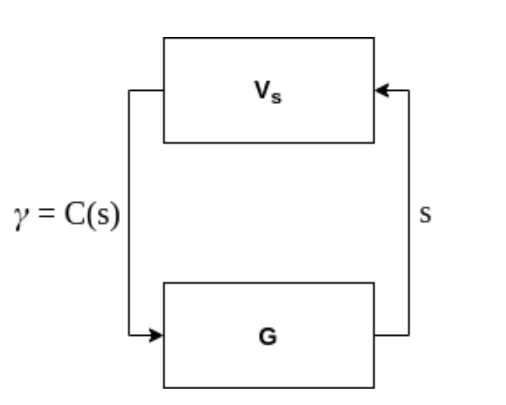
\includegraphics[scale=0.45]{Figures/algoritmo3/desarrollo/retroalimentacion.png} 
	\caption[Retroalimentación entre el  proceso y el supervisor]{Retroalimentación entre el  proceso y el supervisor \footnotemark.}
	\label{fig:fig3.4}
  \end{figure} \footnotetext{Figura adaptada del paper publicado por \textit{D. Kezić} et al. \cite{paperkezic}.}
  
Para alcanzar el control antes mencionado se inicia analizando el grafo de alcanzabilidad en busca de estados con deadlock. En caso de encontrarlos, se continúa con la búsqueda de bad siphons en cada uno de estos.  \\
Ya con todos los estados en deadlock y sus sifones vacíos, se realiza un filtrado de los mismos descartando aquellos que se encuentren vacíos desde el marcado inicial de la red; estos no son de interés para nuestro análisis dado que una vez vacíos (por definición) estos permanecerán en ese estado sin modificar su comportamiento. \\
Una vez realizado el filtrado, se seleccionó uno de los sifones perteneciente a uno de los estados deadlock, y es a este, al que se buscó controlar.

El supervisor que va a controlarlo está compuesto por un conjunto de arcos y por una plaza con un marcado proporcionado por el marcado en el estado inicial (\textit{idle}) del sifón menos uno.
Esto se expresa matemáticamente de la siguiente manera: 

\begin{equation}
    m_0(V_s) = m_0(S_i)-1 
\end{equation}

\noindent El conjunto de arcos vincula la plaza mencionada con tres tipos de transiciones:
\begin{enumerate}
    \item \textbf{Transiciones sensibilizadas en estado idle}: la ejecución de estas transiciones son las que extraen tokens del supervisor dado que el disparo de las mismas inicia los diferentes procesos que componen a la red, pudiendo tomar un camino que conduce al sifón (por lo que el token consumido será devuelto luego de una secuencia de disparos) ó tomar otro camino que no contemple al sifón y en tal caso las transiciones del ítem 3 serán las encargadas de devolver el token consumido al supervisor. 
    
    \item Para el segundo conjunto de transiciones es necesario definir un nuevo conjunto de plazas denominadas \textbf{complemento del sifón}, estas son aquellas plazas que no forman parte del sifón pero para evolucionar en su marcado requieren del disparo de transiciones que se habilitan mediante el marcado de las plazas recurso que componen al sifón, es decir , hacen uso de estas. Es por esto que las transiciones de salidas al conjunto complemento del sifón son aquellas que le agregan tokens al supervisor.
    
    \item Para definir este último conjunto de transiciones se realizó una investigación paralela dado que Ezpeleta no contemplaba este caso. En donde el último arco a tener en cuenta se obtuvo a partir de la relación entre el bad siphon a controlar y los T-invariantes presentes en la red, dependiendo del camino que tome la secuencia de disparos es necesario que este arco devuelva el token al supervisor. \\
    Para esto es necesario verificar la presencia de un conflicto o bifurcación en la red entre T-invariantes, y en caso de existir, enfocarse en las transiciones involucradas en el mismo tal que al dispararse cualquiera de estás no alcancen al sifón, posterior a una secuencia de disparos, ya que el token que se le quitó al supervisor con el disparo de las transiciones idle, mencionadas en ítem 1, nunca volverá a este. \\
    Para corregir esto, con el disparo de la transición conflictiva en cuestión, es necesario implementar el arco que devuelva el token consumido al supervisor. \\
	En caso de dispararse cualquiera de las transiciones del conflicto que posteriormente toman el camino hacía el sifón, no es necesario este arco ya que implica que la extracción por parte de las transiciones idle al supervisor va ser utilizada por la subred formada por el sifón a controlar y los arcos mencionados en el punto 2, los cuales devolverán el token al supervisor.
\end{enumerate}

Tomando la red definida por Ezpeleta se pueden observar los tres tipos de transiciones que conforman el supervisor. El sifón a controlar, en este caso, es el compuesto por las plazas \{$P_7,P_8,P_9,P_{10}$\}.

 \begin{figure}[H]
	\centering
	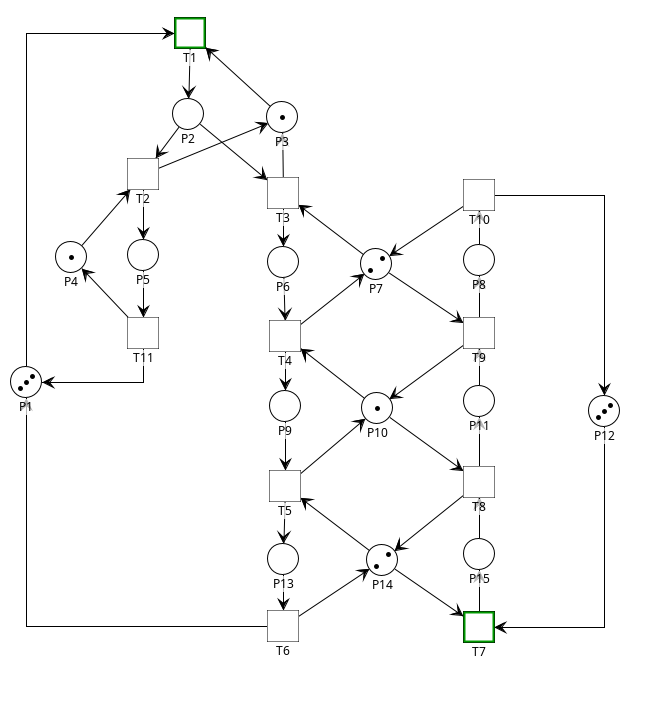
\includegraphics[width=\textwidth]{Figures/algoritmo3/desarrollo/ezpeleta1.png}
	\caption[RdP Ezpeleta.]{RdP Ezpeleta \footnotemark .}
	\label{fig:fig3.5}
  \end{figure} \footnotetext{Figura adaptada del paper publicado por \textit{Ezpeleta} et al. \cite{paperezpeleta} .}

En la figura \ref{fig:fig3.5} se observan las transiciones sensibilizadas en el estado inicial $\{T_1,T_7\}$ , definiendo de esta manera los primeros arcos que componen al supervisor.  
  
 \begin{figure}[H]
	\centering
	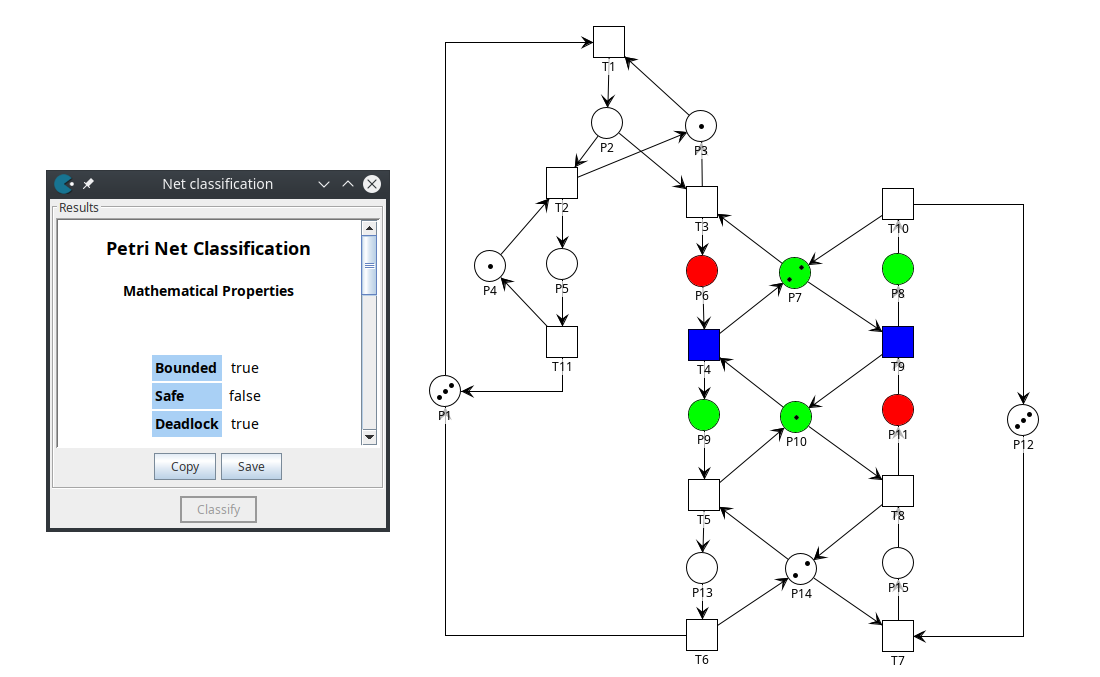
\includegraphics[width=\textwidth]{Figures/algoritmo3/desarrollo/ezpeleta2.png}
	\caption{RdP Ezpeleta con sifón a controlar y sus plazas complemento.}
	\label{fig:fig3.6}
  \end{figure}

Observando la figura \ref{fig:fig3.6} se distingue en verde las plazas que conforman el sifón a controlar y en rojo las plazas complemento del mismo; mientras que en azul las transiciones $\{T_4,T_9\}$ que conectarán con el supervisor mediante el segundo conjunto de arcos. \\


Para definir el tercer tipo de transiciones es necesario tener en cuenta los \break T-invariantes de la red dado que estos nos permiten observar los diferentes caminos que puede tomar la red en la evolución de los disparos de las transiciones de la misma.

 \begin{figure}[H]
	\centering
	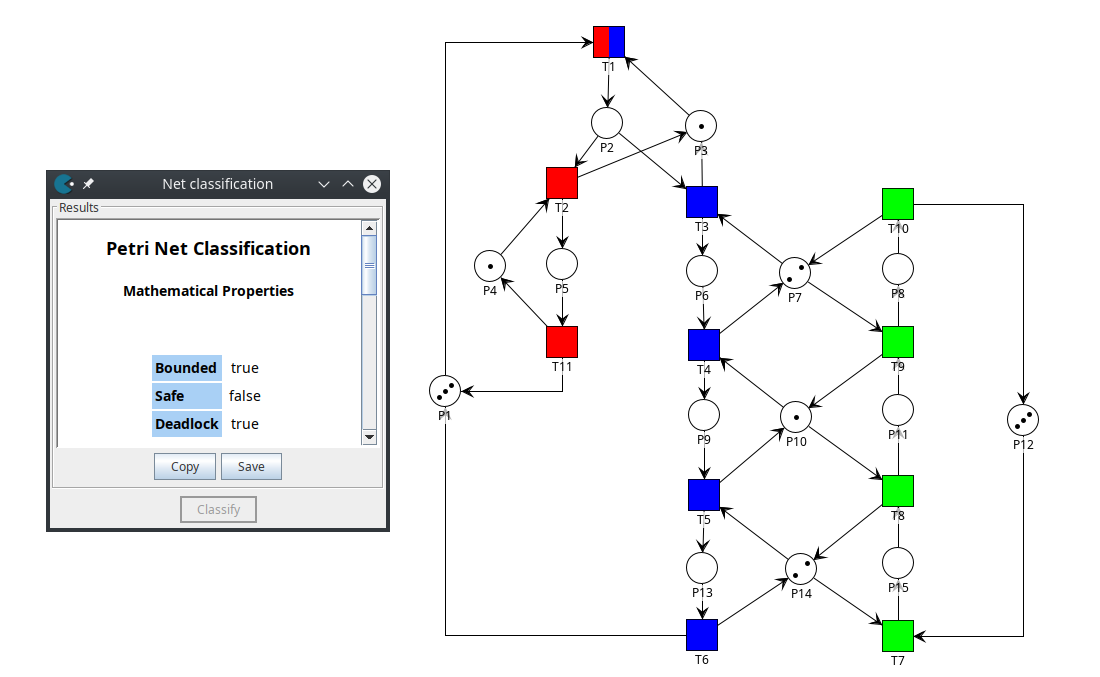
\includegraphics[scale=0.5]{Figures/algoritmo3/desarrollo/ezpeleta3.png}
	\caption{RdP Ezpeleta y sus T-invariantes.}
	\label{fig:fig3.7}
  \end{figure}

Como ilustra la figura \ref{fig:fig3.7}, existen tres invariantes que componen la red (en distintos colores) y la plaza $P_2$ involucrada en un conflicto, dado que su marcado habilita dos posibles caminos de T-invariantes, pudiendo tomar uno u otro. 
En caso de que se proceda con el disparo de la transición $T_2$, produciendo de esta manera la ejecución de las transiciones que componen al T-invariante rojo, el cual no afecta el marcado del sifón en cuestión y por lo que su ejecución devolverá el token al supervisor (se conectara con el supervisor mediante el tercer conjunto de arcos). \\


\noindent Según la definición de la sección \ref{sec:definicionsup}, el supervisor queda conformado de la siguiente manera:
\begin{itemize}
    \item El marcado = $ M(S_i) - 1 = \{M(P_7) + M(P_8) + M(P_9) + M(P_{10}) \} -1 = 2$ 
    \item Transiciones output = $\{T_1, T_7\}$
    \item Transiciones input = $\{T_2, T_4, T_9\}$
\end{itemize}

\begin{figure}[H]
    \centering
    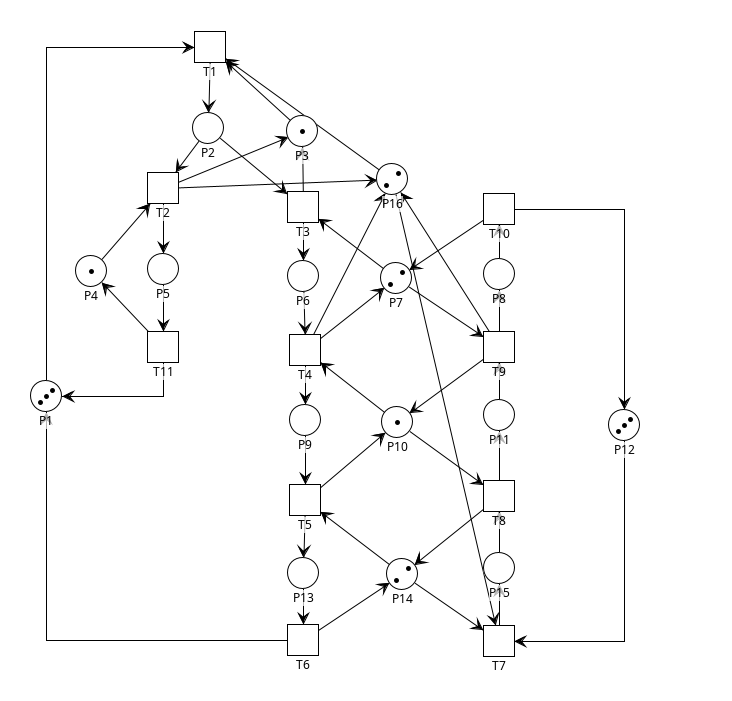
\includegraphics[scale=0.7]{Figures/algoritmo3/desarrollo/ezpeleta4.png}
    \caption{Colocación de un supervisor en RdP Ezpeleta.}
    \label{fig:fig3.8}
 \end{figure}

Por último, en la figura \ref{fig:fig3.8}, se observa la red al controlar uno de los bad siphon, este control se logra al colocar el supervisor ($P_{16}$) con su marcado y arcos respectivos. \\


\noindent El análisis completo de la red se llevará a cabo en las iteraciones posteriores dado que la red aún presenta deadlock.


\subsection{Implementación del algoritmo}
En esta sección se desarrollan los 5 pasos que modelan el algoritmo en la determinación del supervisor. \\
Una de las consideraciones a tener en cuenta, la cuál emerge del estudio de las distintas redes simétricas es:
\begin{itemize}
    \item En caso de que la red a controlar fuese simétrica, aislar en subredes y ejecutar el algoritmo en una sola de ellas obteniendo el control de la misma; el cual se podrá extender a las restantes partes. Teniendo en cuenta, al momento de integrarlas en la red completa, que los arcos pertenecientes al supervisor de cada una de las partes deben aplicarse de igual manera a los supervisores de las otras subredes (como puede observarse en el caso de la red Portugal (sección \ref{sub:portugal})). %Vincular cuando este terminado con la sección.
\end{itemize}

\newpage
\subsubsection{Desarrollo} \label{sec:desarrollov3}
\begin{enumerate}
    \item Obtener los sifones vacíos en el estado inicial; estos sifones deben ignorarse dado que una vez vacíos permanecerán así por el resto de los estados alcanzables.
    \item Obtener los estados en deadlock con sus respectivos sifones vacíos. 
    \item Seleccionando uno de los sifones mencionados en el ítem anterior:
        \begin{enumerate}
            \item Se obtiene su marcado inicial para posteriormente definir el marcado de su correspondiente supervisor.
            \item Se localizan las transiciones sensibilizadas en el estado idle (para el marcado inicial). 
            \item Se obtienen las plazas complemento del mismo.
                \begin{enumerate}[i. ]
                    \item Se buscan las transiciones que quitan y agregan tokens a estas plazas. 
                    \item Las transiciones que agregan más tokens de los que quitan al sifón son las que nos interesan.
                \end{enumerate}
            \item Se verifica si hay transiciones en conflicto, de ser así se utilizan los \break T-invariantes para verificar si la ejecución de la misma se encuentra en el camino de las plazas del sifón. De no ser así, estas transiciones serán también de interés.
        \end{enumerate}
    Las transiciones destacadas en los ítems anteriores van a ser las que van a incorporar y extraer tokens del supervisor, como se mencionaron en la iteración 2.

    \item Agregar una nueva plaza de control (perteneciente al supervisor) a la red puede producir un nuevo sifón mínimo no controlado y un nuevo estado de bloqueo. Por lo tanto, debemos volver al punto 1 calculando nuevamente el árbol de alcanzabilidad y repetir todo el algoritmo, atacando la totalidad de los bad siphon hasta alcanzar una red viva. \\
    El algoritmo finaliza cuando no es posible encontrar un nuevo punto muerto en la red de Petri, es decir se resuelve el deadlock de la misma. \\ Sin embargo, puede darse la situación en donde el algoritmo no converge a una solución dado que sugiere supervisores con marcado igual a 0 o supervisores ya colocados.

    \item En caso, de que los pasos anteriores no convergen a una red libre de deadlock se realiza un análisis de división de la misma y se ataca cada subred resultante por separado, es decir, se debe ejecutar el algoritmo desde el paso 1 al 4 para cada subred, para luego reunir las soluciones en la red de petri original. \\
    La división se realiza teniendo en cuenta los T-invariantes y su relación con los bad siphon.

    Para esto se deben tener en cuenta algunos factores:        
    \begin{enumerate}
            \item En caso de que la división de la red resulte en una de las subredes que contempla el conflicto en su totalidad (caso red POPN (sección \ref{sub:POPN})), las soluciones de ambas subredes se pueden unir conservando la vivacidad de la red sin problema. 
            
            \item En caso de ser necesaria la división en subredes y la misma no pueda contemplar el conflicto en su totalidad (caso red Hospital (sección \ref{sub:Hospital})), notar que las transiciones pertenecientes al conflicto deben devolver el token, al momento de unir las subredes, al supervisor que no es propio de su subred; debiendo colocar de esta manera un nuevo arco en la red original. 
        \end{enumerate} %Agregar la sección luego
    En caso de tener supervisores en común entre las subredes, es decir, tienen el mismo conjunto de arcos entrantes y salientes, al momento de definir el marcado del mismo en la red original, el supervisor debe tomar el valor del marcado del menor de ellos dado que no tiene que permitir el vaciado del sifón con menos marcas.
\end{enumerate}


\noindent Las fórmulas para calcular el supervisor para un sifón son las siguientes:
\begin{enumerate}
    \item $m(V_s) = m(BS_i) - 1$
    \item $Arco_1 = \{(V_s, t) \ / \ t \in P_0 \bullet \}$
    \item $Arco_2 = \{(t, V_s) \ / \ t \in C_s \bullet \}$
    \item $Arco_3 = \{(t, V_s) \ / \ t \in conflicto \wedge t \notin T_{inv_{BS_i}} \}$
\end{enumerate}

\noindent siendo:
\begin{enumerate}
    \item $V_s$ = plaza supervisor
    \item $P_0$ = plazas marcadas idle
    \item $C_s$ = complemento sifón
    \item $BS_i$ = bad siphon
    \item $t$ = conjunto de transiciones
\end{enumerate}

En la figura \ref{fig:fig3.9} se puede observar, a modo de ejemplo de aplicación, la salida del algoritmo por consola para la ejecución de la red de Petri Panamá, analizada en profundidad en sección 3.4.3.3.

\begin{figure}[H]
	\centering
	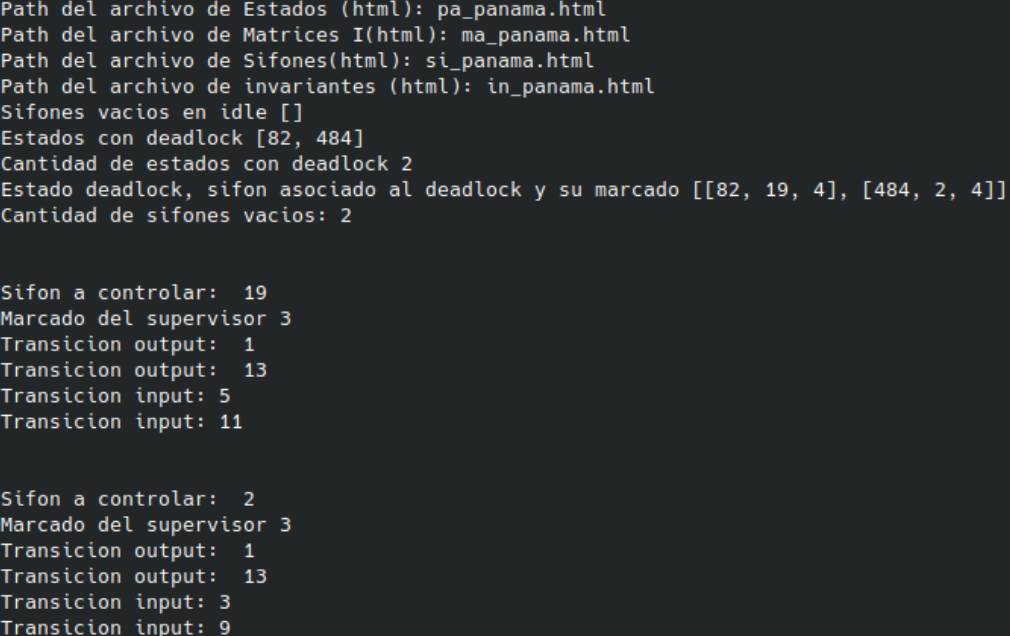
\includegraphics[scale=0.5]{Figures/algoritmo3/desarrollo/consola.png}
	\caption{Ejecución del algoritmo v3.0.}
	\label{fig:fig3.9}
 \end{figure}

\begin{enumerate}[i.]
    \item Las primeras 4 líneas son para la conversión de los datos exportados mediante el software Petrinator:
        \begin{itemize}
            \item \textit{pa\_panama.html} contiene el grafo de alcanzabilidad.
            \item \textit{ma\_panama.html} contiene la matriz pre y post.
            \item \textit{si\_panama.html} contiene los sifones y las trampas.
            \item \textit{in\_panama.html} contiene los invariantes de plaza y de transición.
        \end{itemize}
    
    \item En este caso no fue necesario descartar ningún sifón en el análisis dado que en el estado inicial todos los sifones se encuentran marcados. 
    
    \item Se obtienen los estados en deadlock con sus respectivos sifones vacíos y el marcado de los mismos.
    
    \item Como se puede observar el algoritmo brinda todos los posibles supervisores para el control de los sifones vacíos en deadlock. 
\end{enumerate}

Se toma uno de los supervisores, se incorpora a la red en el software Petrinator realizando el análisis correspondiente en búsqueda de verificar que el deadlock de la red haya desaparecido; de no ser así se exportan nuevamente los archivos y se realiza la ejecución del algoritmo nuevamente. Y así iterativamente hasta lograr que el deadlock de la red desaparezca.

\subsubsection{Pseudocódigo}
\noindent Definiendo:
\begin{itemize}
    \item $C_S$: complemento del sifón
    \item t: conjunto de transiciones
    \item $V_S$: plaza supervisor
    \item Cantidad de sifones = cantidades de sifones total del sistema
    \item SD: state deadlock
    \item S: conjunto de sifones
    \item BS: conjunto de bad siphons
\end{itemize}

\begin{algorithm} [H]
  \floatname{algorithm}{Pseudocódigo}
  \caption{búsqueda de bad siphon a controlar (v3)}
  \label{alg:algoritmo1} 
  \begin{algorithmic}[1]
 
    % ENTRADA / SALIDA
    \Require{RdP ($N,M_0$) de tipo S³PR.}
    \Ensure{bad siphon.}
 
    \State Generar el grafo de alcanzabilidad G($N,M_0$) de la RdP.
    \State Obtener matrices I+, I-, invariantes, trampas y sifones.
 
    \For{i: 0 \textbf{to} cantidad de estados}
        \If{estado = estado en deadlock}
            \State $SD_j$ $\leftarrow$ \ $estado_i$
        \EndIf
    \EndFor
    
    \If{estado =  idle}
        \For{i: 0 \textbf{to} cantidad de sifones}
            \If{M($S_i$) = 0}
                \State $BS_{idle}$ $\leftarrow$ \  $S_i$
            \EndIf
        \EndFor
    \EndIf
    
    \State en SD[0]
    \For{i: 0  \textbf{to}  cantidad de sifones}
        \If{$M(S_i)$ = 0}
            \State $BS_{SD}$ $\leftarrow$ \ $S_i$  
        \EndIf
    \EndFor
    \State Se eliminan de $BS_{SD}$ aquellos que estén en $BS_{idle}$ 
    \State $BS_{SD}$[0] \  $\rightarrow$\ control de bad siphon usando \textbf{Algoritmo \ref{alg:algoritmo2}}
  \end{algorithmic}
\end{algorithm}
\bigskip

\begin{algorithm}[H] 
  \floatname{algorithm}{Pseudocódigo}
  \caption{Búsqueda de supervisor que controle bad siphon (v3)}
  \label{alg:algoritmo2} 
  \begin{algorithmic}[1]
 
    % ENTRADA / SALIDA
    \Require{RdP ($N,M_0$) de tipo S³PR.}
    \Ensure{supervisor.}
 
    \State \textbf{Agregar} plaza de control $VS_i$ con $M(VS_i)= M(BS_{SD}) - 1$
    
    \If{estado = idle}
            \State \textbf{Agregar} arco $(VS_i , t) \ \forall \  t \in \ p\bullet$
    \EndIf
 
    \State \textbf{Agregar} arco $(t, VS_i) \forall \ t \in \ C_S\bullet$
    \State \textbf{Agregar} arco $(t, VS_i)  \forall \ t \in \ conflicto \ \wedge \ t \notin T-invariante_{BS}$
  \end{algorithmic}
\end{algorithm}
\bigskip

El algoritmo iterativo para lograr una red de Petri sin deadlock se muestra en la figura \ref{fig:fig3.10}

\begin{figure}[H]
	\centering
	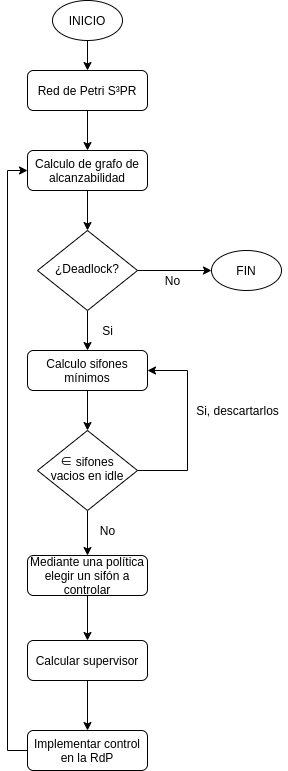
\includegraphics[scale=0.5]{Figures/algoritmo3/desarrollo/diagrama_flujo.png}
	\caption{Ejecución del algoritmo v3.0.}
	\label{fig:fig3.10}
 \end{figure}

\subsection{Criterio de elección del supervisor} \label{sec:criterio}
Al ejecutar el algoritmo, se obtiene una lista de supervisores a colocar dependientes al bad siphon que se va a controlar. El criterio de elección de qué supervisor agregar se realiza teniendo en cuenta: 
\begin{itemize}
    \item Afecte a un sifón mínimo.
    \item Cantidad de veces que aparece el supervisor en la lista.
    \item En caso de haber más de un supervisor sugerido para el control de un bad siphon, se elige aquel que presente la menor cantidad de \textit{inputs}.
\end{itemize}


\subsection{Ejecución en diferentes escenarios}
En esta sección se busca explicar cómo fue progresando el algoritmo a medida que se implementó en diferentes casos de redes de Petri, dado que en cada nueva red se encontraban situaciones diferentes que debían tenerse en cuenta y cada una implicó una extensión más para el algoritmo final. \\
Estas extensiones se deben a que en cada una de las redes analizadas la relación que presentaban sus T-invariantes con el bad siphon a controlar era diferente, esto fue lo que permitió generalizar el algoritmo de manera de contrarrestar el deadlock en cada una de las variantes.

\subsubsection{Caso Panamá}
Esta red modela un sistema de tráfico marino. El problema es la posibilidad de interbloqueo entre los barcos que circulan a través de un sistema de canales y dársenas (tres canales y cuatro dársenas). Los barcos circulan hacia la derecha o izquierda, esperando a cada lado del sistema de canales su derecho a paso. 
La capacidad de cada canal y dársena es de un barco a la vez, por lo que un barco no puede ingresar a un canal o dársena ocupado, estando obligado a esperar a que se desocupe.

\begin{figure}[H]
    \centering
    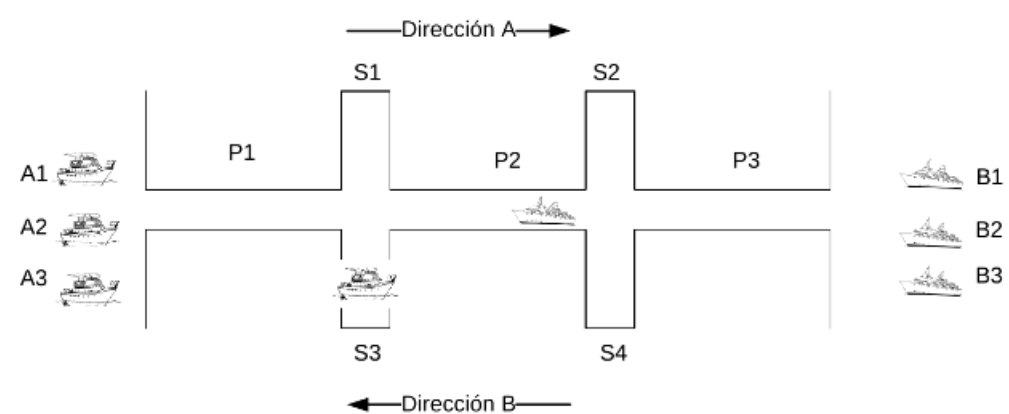
\includegraphics[width=\textwidth]{Figures/algoritmo3/panamacanal.png}
    \caption[Modelo del Canal de Panamá.]{Modelo del Canal de Panamá \footnotemark.}
    \label{fig:fig3.11}
 \end{figure} \footnotetext{Figura adaptada del libro \textit{An  Algorithm  for  Deadlock Prevention  Based  on  Iterative  Siphon  Control  of  Petri  Net} \cite{paperpanama} .}

\paragraph{Características generales}
\begin{itemize}
    \item Las cuatro dársenas están representadas por las plazas \{$P_{15}, P_{16}, P_{17}, P_{18}$\}.
    \item Los tres canales se denotan por las plazas \{$P_{19}, P_{20}, P_{21}$\}.
    \item Mientras que los barcos por las marcas de las plazas \{$P_1, P_7$\}.
\end{itemize}

\newpage
\paragraph{Análisis estructural}
\hfill
\begin{figure}[H]
	\centering
    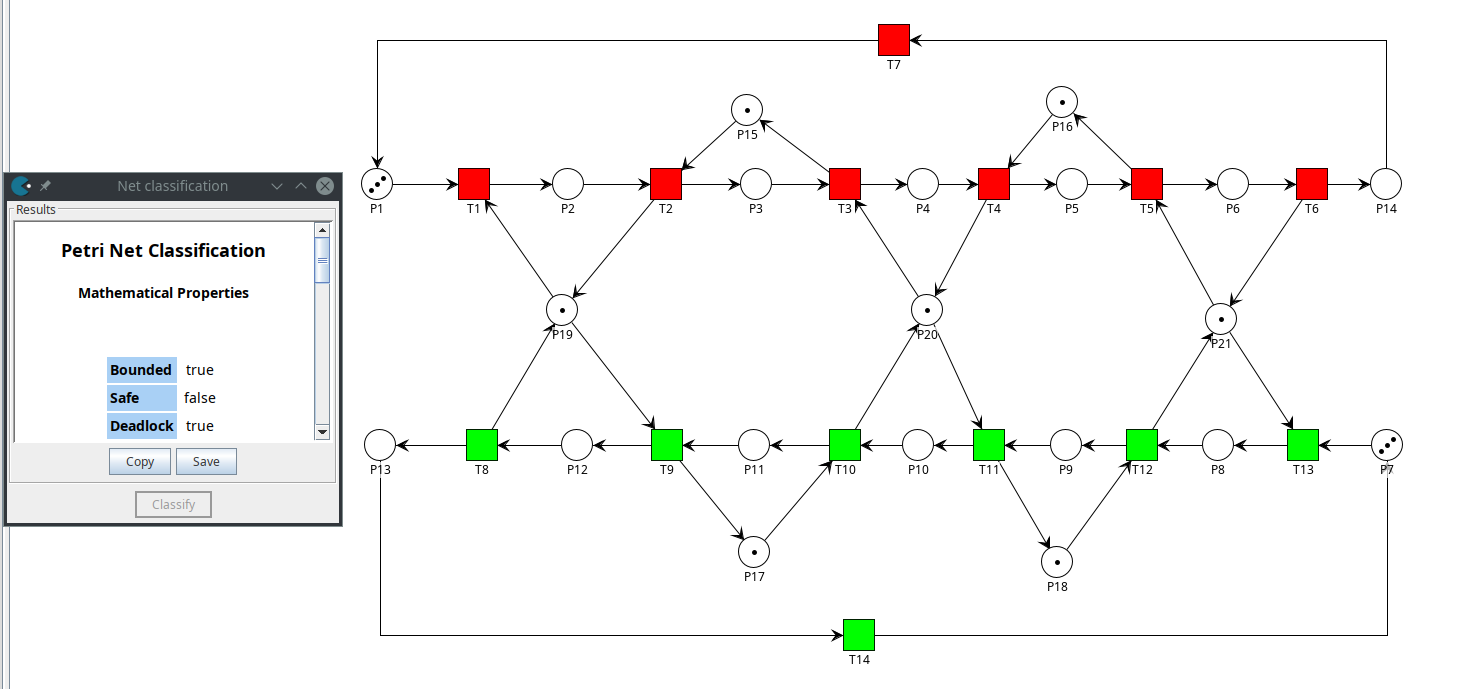
\includegraphics[scale = 0.41]{Figures/algoritmo3/Panama1.png}
    \caption[RdP Canal de Panamá y sus T-invariantes.]{RdP Canal de Panamá \footnotemark \ y sus T-invariantes.}
	\label{fig:panamaytinvariantes}
 \end{figure} \footnotetext{Figura adaptada del libro \textit{An  Algorithm  for  Deadlock Prevention  Based  on  Iterative  Siphon  Control  of  Petri  Net} \cite{paperpanama} .}
 
\hfill \par En la figura \ref{fig:panamaytinvariantes}, la red no presenta un conflicto entre los T-invariantes, representados en rojo y verde. Se ejecuta el algoritmo desde el punto 1 al 4 permitiendo encontrar los supervisores sin necesidad de subdividir la red; incluso realizar esta acción en esta red no tendría mucho sentido dado que los T-invariantes por separado no representan el comportamiento de la red en su totalidad.

\paragraph{Red controlada}
\hfill  
\par Una vez ejecutado el algoritmo, se obtienen los supervisores a agregar para controlar la red solucionando el deadlock, estos están representado por las plazas $P_{22}$ y $P_{23}$ en la figura \ref{fig:panamaytinvariantes}.

\begin{table}[H]
    \centering
    \begin{tabular}{|c|c|P{2.2cm}|P{2.2cm}|c|}
    \hline
    \textbf{Supervisor} & \textbf{Marcado} & \textbf{Transiciones input} & \textbf{Transiciones output} & \textbf{Bad Siphon Controlado}  \\  \hline
    $P_{22}$ & 3 & \{$T_{5}, T_{11}$\} & \{$T_{1}, T_{13}$\} & \{$P_6,P_{10},P_{16},P_{18},P_{20},P_{21}$\} \\ 
    \hline
    $P_{23}$ & 3 & \{$T_{3}, T_{9}$\} & \{$T_{1}, T_{13}$\} & \{$P_4,P_{12},P_{15},P_{17},P_{19},P_{20}$\} \\ 
    \hline
    \end{tabular}
    \caption{Supervisores: RdP Panamá.}
    \label{tab:panama}
    
    \end{table}

\begin{figure}[H]
	\centering
	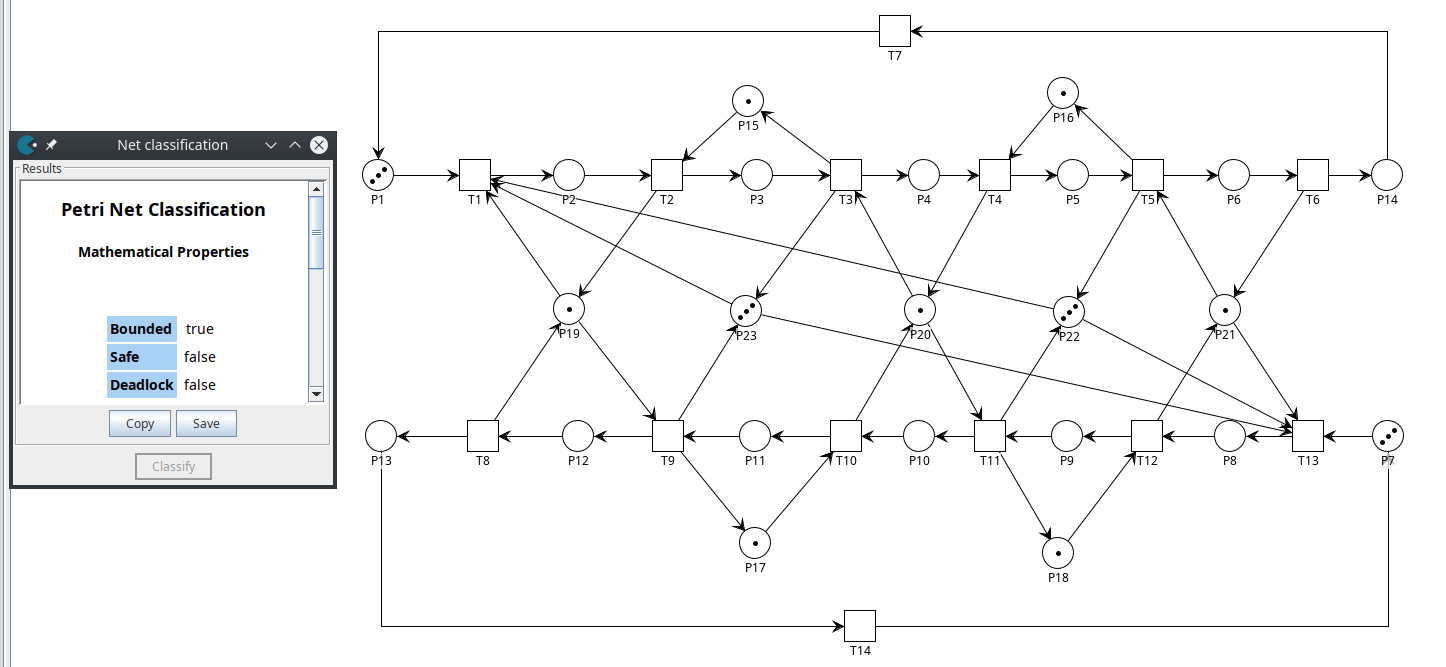
\includegraphics[scale=0.4]{Figures/algoritmo3/Panama2.png}
	\caption{RdP Canal de Panamá controlada.}
	\label{fig:panamacontrolada}
 \end{figure}
 
 \subsubsection{Caso Ezpeleta}
Esta red modela la ejecución concurrente de procesos de trabajo en FMS, representando un sistema donde se ejecutan dos tipos de procesos de trabajo. \\
En la red existen plazas que simulan la disponibilidad de recursos (5) y un control incorrecto de estos en la ejecución de los procesos de trabajo, puede conducir a situaciones de deadlock.

\paragraph{Características generales}
\begin{itemize}
    \item Presenta conflicto entre T-invariantes.
    \item Los recursos de la red están representados por las plazas \{$P_3,P_4,P_7,P_{10},P_{14}$\}.
\end{itemize}

\paragraph{Análisis estructural}
\hfill
\begin{figure}[H]
	\centering
	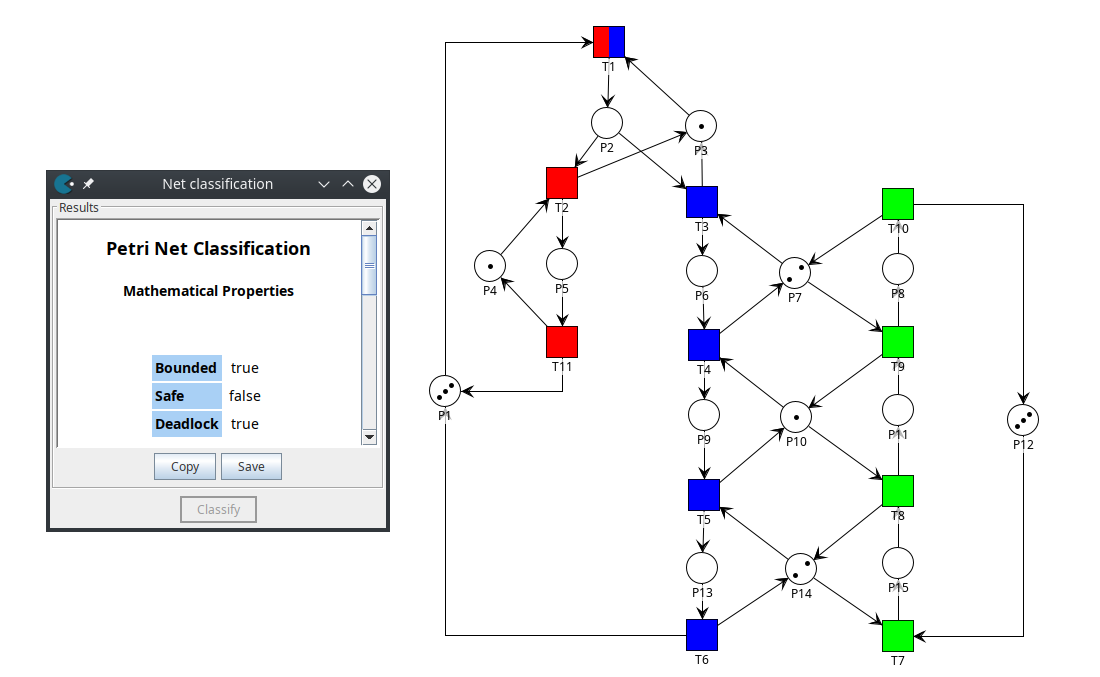
\includegraphics[scale=0.5]{Figures/algoritmo3/ezpeleta1.png}
	\caption[RdP Ezpeleta y sus T-invariantes.]{RdP Ezpeleta \footnotemark \ y sus T-invariantes.}
	\label{fig:ezpeletatinvariante}
 \end{figure} \footnotetext{Figura adaptada del paper publicado por \textit{Ezpeleta} et al. \cite{paperezpeleta}.}

En la figura \ref{fig:ezpeletatinvariante}, la plaza $P_2$ forma parte de un conflicto permitiendo la ejecución de un subcircuito de la red u otro, pudiendo seguir dos T-invariantes diferentes (rojo o azul en este caso). \\
Es por esto que fue necesario ejecutar el algoritmo de forma completa, es decir, desde el punto 1 al 5, contemplando la división de la red dado que los primeros 4 pasos no lograron alcanzar una red libre de deadlock.\\
En la división resultaron dos subredes, ambas preservando el conflicto (plaza y transiciones que lo conforman).

\subparagraph{Subred izquierda}
\hfill \break
Una de las subredes (figura \ref{fig:ezpeletasubizquierda}) no fue necesario controlarla dado que no presentaba deadlock.

\begin{figure}[H]
	\centering
	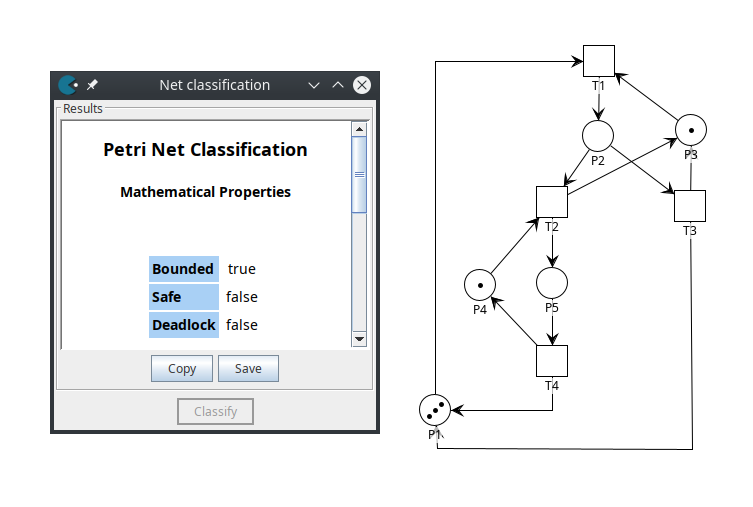
\includegraphics[scale=0.55]{Figures/algoritmo3/ezpeleta2.png}
	\caption{Subred izquierda Ezpeleta.}
	\label{fig:ezpeletasubizquierda}
 \end{figure}

\subparagraph{Subred derecha}
\hfill \break
Mientras que la segunda subred (figura \ref{fig:ezpeletasubderecha}) si fue necesario encontrar los supervisores que resuelvan el deadlock. \\
\bigskip

\begin{figure}[H]
	\centering
	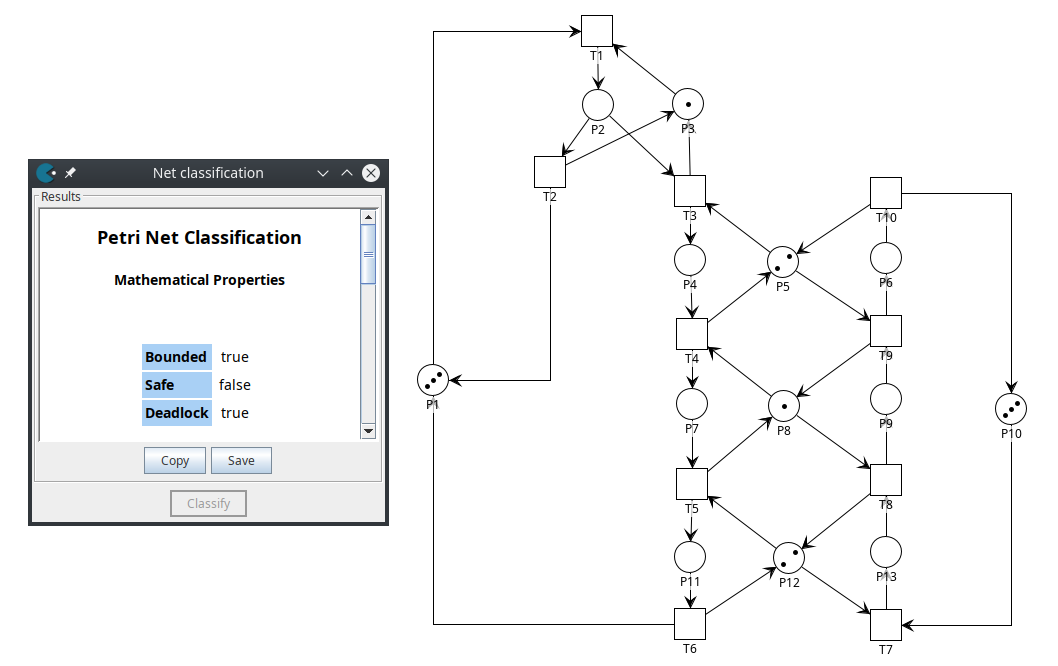
\includegraphics[scale=0.5]{Figures/algoritmo3/ezpeleta3.png}
	\caption{Subred derecha Ezpeleta.}
	\label{fig:ezpeletasubderecha}
 \end{figure}
\bigskip

\subparagraph{Control subred derecha}
\hfill \break
Una vez ejecutados los 4 primeros pasos del algoritmo, sobre la subred en cuestión, se obtuvieron los supervisores a agregar para controlar la misma, resolviendo el problema de punto muerto. \\
\bigskip

\begin{table}[H]
    \centering
    \begin{tabular}{|c|c|P{2.2cm}|P{2.2cm}|c|}
   \hline
    \textbf{Supervisor} & \textbf{Marcado} & \textbf{Transiciones input} & \textbf{Transiciones output} & \textbf{Bad Siphon Controlado}  \\  \hline
    $P_{15}$ & 4 & \{$T_{2}, T_{5}, T_{9}$\} & \{$T_{1}, T_{7}$\} & \{$P_5,P_{6},P_{8},P_{11},P_{12}$\} \\ 
    \hline
    $P_{14}$ & 2 & \{$T_{2}, T_{5}, T_{8}$\} & \{$T_{1}, T_{7}$\} & \{$P_8,P_{9},P_{11},P_{12}$\} \\ 
    \hline
    $P_{13}$ & 2 & \{$T_{2}, T_{4}, T_{9}$\} & \{$T_{1}, T_{7}$\} & 
    \{$P_5,P_{6},P_{7},P_{8}$\} \\ 
    \hline
    \end{tabular}
    \label{tab:ezpeletaderecha}
    \caption{Supervisores: RdP Ezpeleta (R).}
\end{table}

\begin{figure}[H]
	\centering
	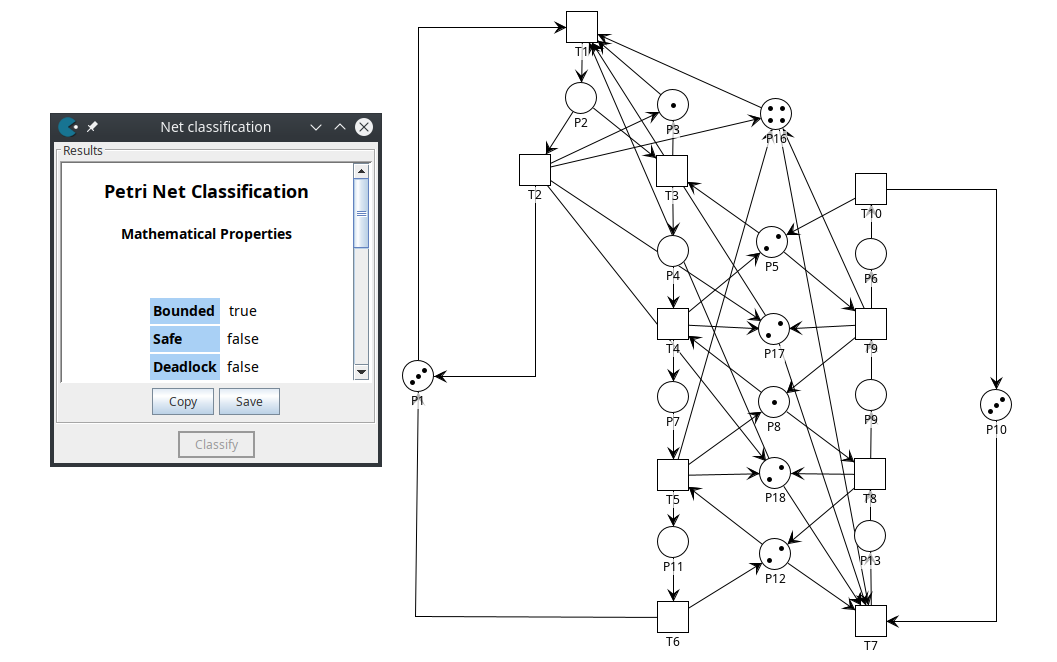
\includegraphics[scale=0.55]{Figures/algoritmo3/ezpeleta4.png}
	\caption{Subred derecha Ezpeleta controlada.}
	\label{fig:ezpeletasubderechacontrolada}
 \end{figure}

\subparagraph{Control red original}
Al contemplar el conflicto en el análisis de cada subred por separado, la unión de estas soluciones permiten resolver el deadlock de la red completa, sin necesidad de realizar otro análisis.\\

\begin{figure}[H]
	\centering
	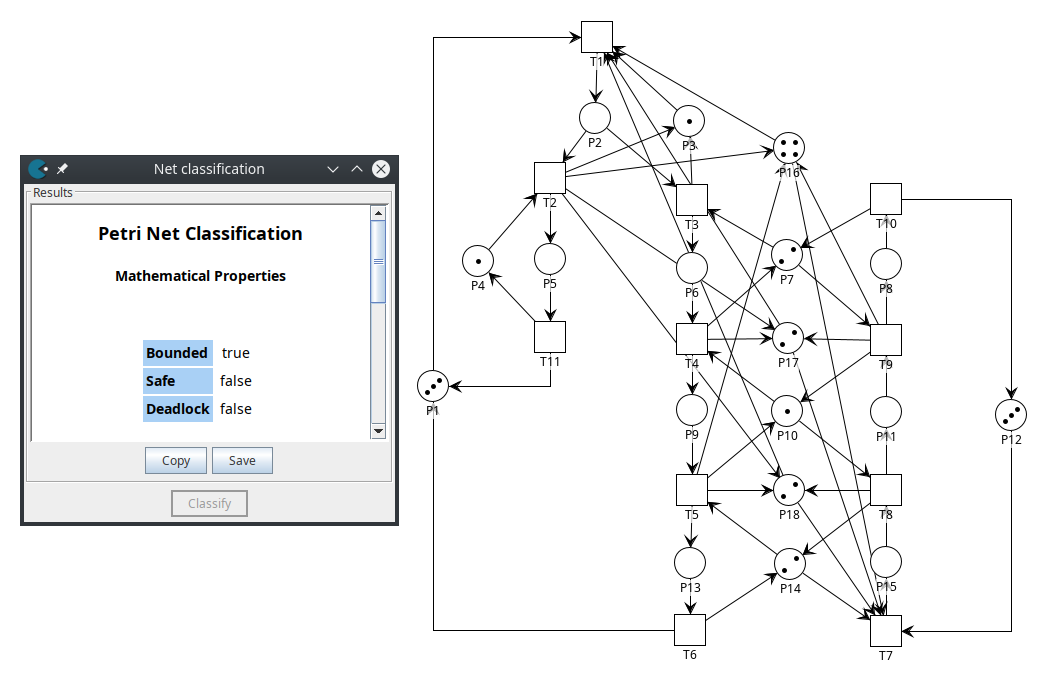
\includegraphics[scale=0.55]{Figures/algoritmo3/ezpeleta5.png}
	\caption{RdP Ezpeleta controlada.}
	\label{fig:ezpeletacontrolada}
 \end{figure}

\subsubsection{Caso POPN} \label{sub:POPN}
Esta red modela un sistema de manufacturación robotizado que consiste principalmente de: tres robots {R1, R2, R3} y cuatro máquinas {M1, M2, M3, M4}.\\
En este sistema se procesan tres tipos diferentes de piezas A, B y C; estas provienen de tres contenedores de entrada distintos I1, I2 e I3, de los cuales los robots las retiran, las colocan en las máquinas para su procesamiento y posteriormente depositan en tres contenedores de salidas distintos, que son: O1, O2 y O3. \\
Todo esto se puede visualizar en figura \ref{fig:popnrobot}.

\begin{figure}[H]
	\centering
	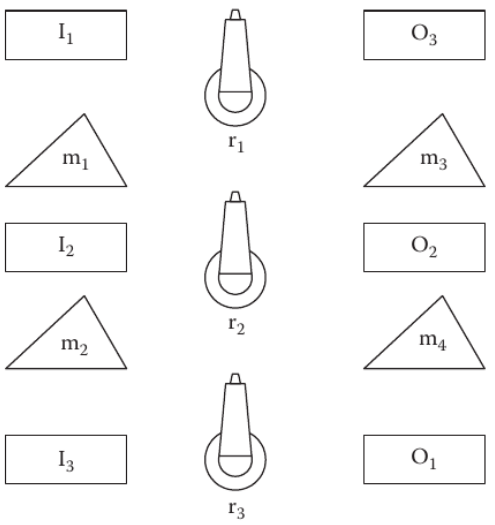
\includegraphics[scale=0.55]{Figures/algoritmo3/POPNrobot.png}
	\caption[Modelado de partes del sistema POPN.]{Modelado de partes del sistema POPN\footnotemark .}
	\label{fig:popnrobot}
 \end{figure} \footnotetext{Figura adaptada del libro \textit{System Modeling and Control with Resource-OrientedPetri Nets} \cite{libropopn}.}

Los robots tienen tareas definidas, cada operación de traslado de las piezas le corresponde a un único robot. \\
En la figura \ref{fig:popnrobotlinea}, se observan las tres trayectorias diferentes para cada tipo de pieza.

\begin{figure}[H]
	\centering
	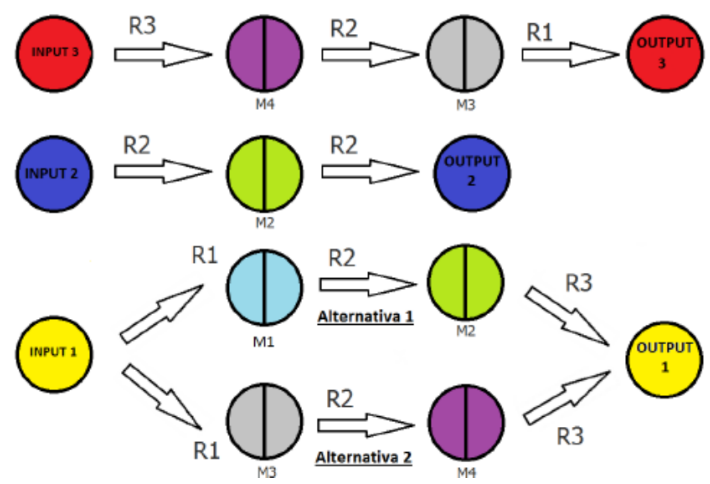
\includegraphics[scale=0.55]{Figures/algoritmo3/POPNrobotlinea.png}
	\caption{Trayectorias de la producción de las piezas.}
	\label{fig:popnrobotlinea}
 \end{figure} 

Cada una de las máquinas, M1, M2, M3 y M4, tiene un color diferente. Y R1, R2 y R3 representan a los tres robots del sistema, encargados de trasladar las piezas de un lado a otro, hasta llegar a su objetivo. Si los recursos no se distribuyen de la forma correcta entre las máquinas la red se bloquea.

\paragraph{Características generales}
    \begin{itemize}
        \item Presenta conflicto entre T-invariantes.
        \item Las máquinas M1-M4 estan representadas por $\{P_8, P_9, P_{21}, P_{22}\}$
        \item Mientras que los recursos R1-R3 están denotados por $\{P_7, P_{14}, P_{10}\}$
    \end{itemize}
   
\paragraph{Análisis estructural}
\hfill \break

\begin{figure}[H]
	\centering
	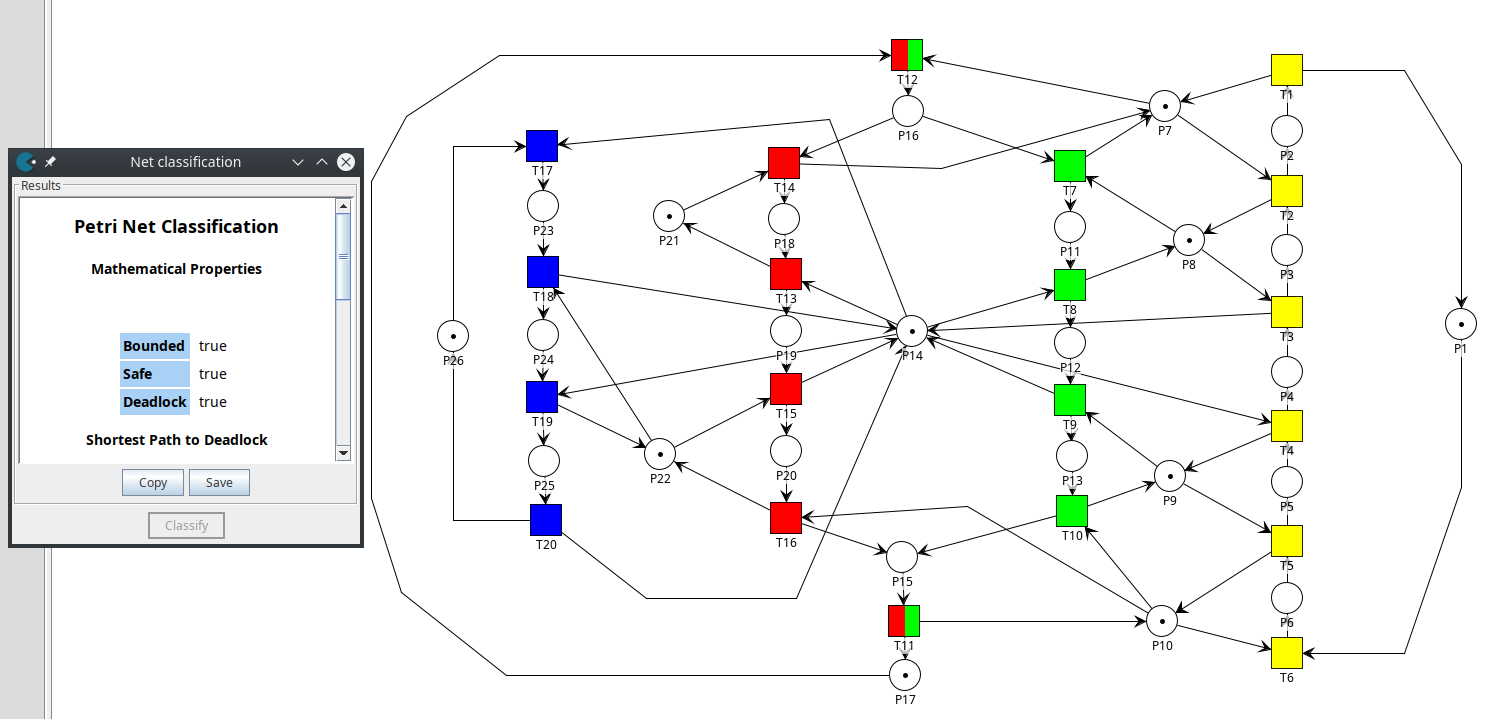
\includegraphics[width=\textwidth]{Figures/algoritmo3/POP1.png}
	\caption[RdP POPN y sus T-invariantes.]{RdP POPN \footnotemark \ y sus T-invariantes.}
	\label{fig:popntinvariantes}
 \end{figure} \footnotetext{Figura adaptada del libro \textit{System Modeling and Control with Resource-OrientedPetri Nets} \cite{libropopn} .}

En la figura \ref{fig:popntinvariantes}, la plaza $P_{16}$ forma parte de un conflicto, permitiendo la ejecución de un subcircuito de la red u otro, pudiendo seguir dos T-invariantes diferentes (rojo o verde en este caso).
Es por esto que fue necesario ejecutar el algoritmo de forma completa, es decir desde el punto 1 al 5, contemplando la división de la red dado que los primeros 4 pasos no lograron alcanzar una red libre de deadlock.\\
De la división resultaron dos subredes, preservando el conflicto (plaza y transiciones que lo conforman) en cada una de ellas.

\subparagraph{Subred derecha}
\hfill
\begin{figure}[H]
	\centering
	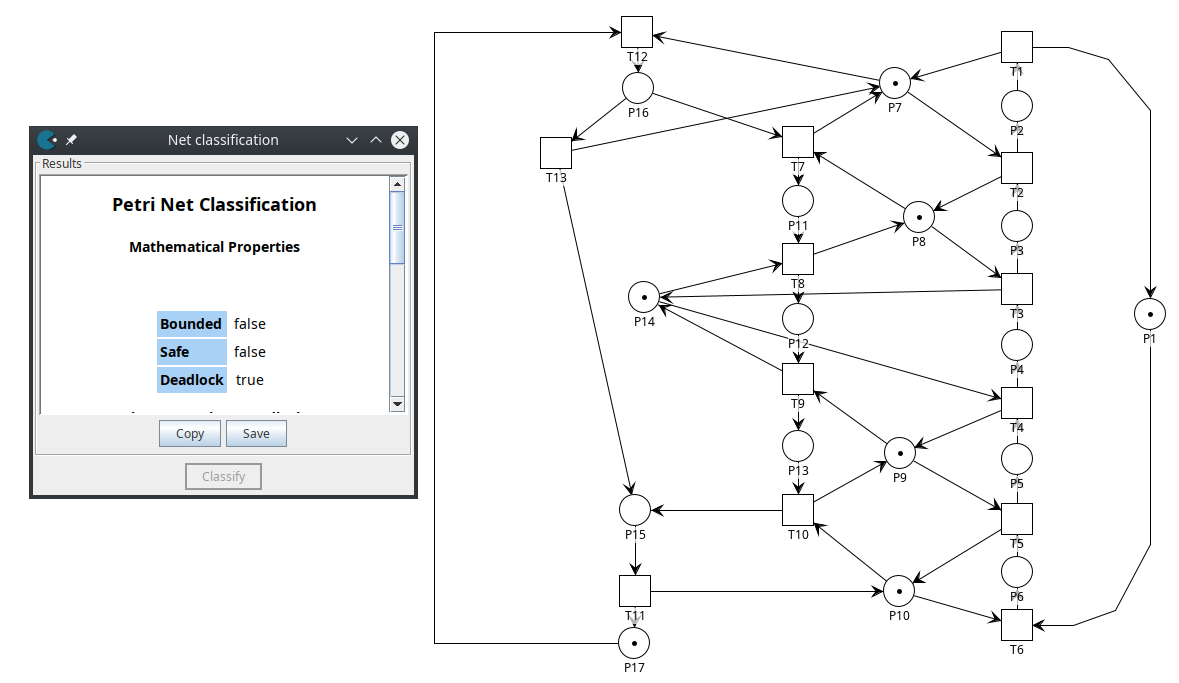
\includegraphics[scale=0.48]{Figures/algoritmo3/POP2.png}
	\caption{Subred derecha POPN.}
	\label{fig:popnredder}
 \end{figure}

\subparagraph{Subred izquierda}
\hfill
\begin{figure}[H]
	\centering
	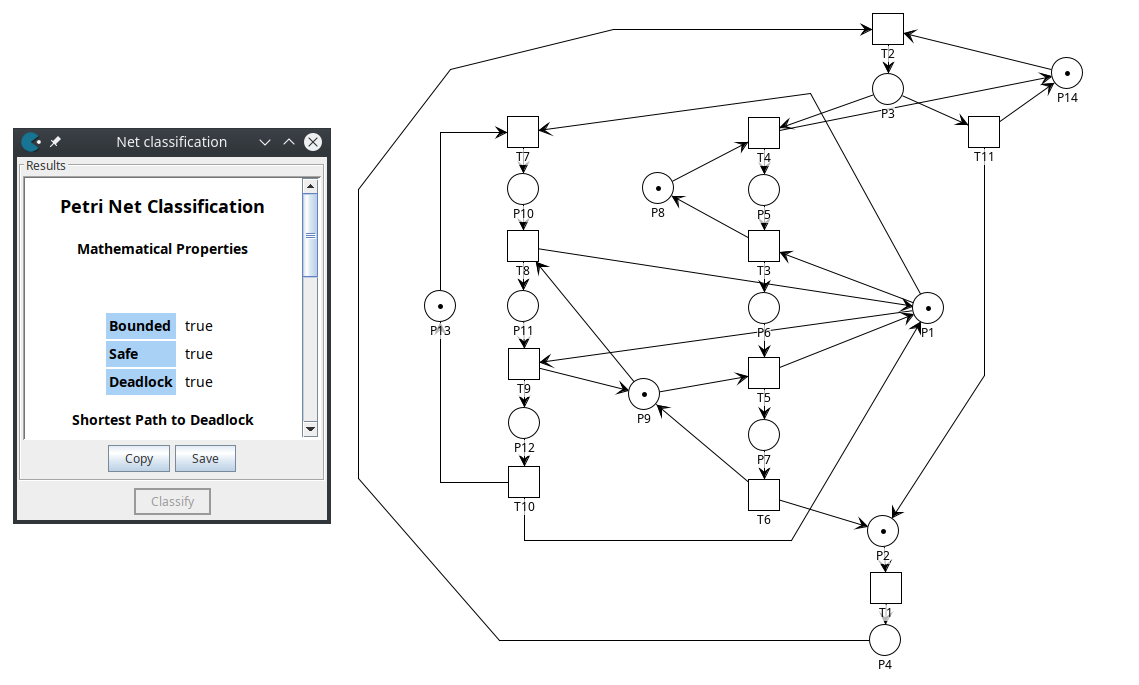
\includegraphics[scale=0.5]{Figures/algoritmo3/POP3.png}
	\caption{Subred izquierda POPN.}
	\label{fig:popnredizq}
 \end{figure}
\bigskip

Dado que ambas subredes presentan deadlock es necesario ejecutar el algoritmo en cada una de ellas (desde el paso 1 al 4). 
\bigskip

\newpage
\subparagraph{Control de subredes}
\hfill \break
En las siguientes figuras \ref{fig:popnreddercontrolada} y \ref{fig:popnredizqcontrolada} se puede observar el control logrado en cada una de las subredes:\\ 
\bigskip

\begin{table}[H]
    \centering
    \begin{tabular}{|c|c|P{2.2cm}|P{2.2cm}|c|}
    \hline
    \textbf{Supervisor} & \textbf{Marcado} & \textbf{Transiciones input} & \textbf{Transiciones output} & \textbf{Bad Siphon Controlado}  \\  \hline
    $P_{28}$ & 1 & \{$T_{3}, T_{8}, T_{14}$\} & \{$T_{6}, T_{12}$\} & \{$P_3,P_{8},P_{12},P_{14}$\} \\
    \hline
    $P_{29}$ & 1 & \{$T_{4}, T_{9}, T_{14}$\} & \{$T_{6}, T_{12}$\} & \{$P_4,P_{9},P_{13},P_{14}$\} \\
    \hline
    $P_{30}$ & 1 & \{$T_{5}, T_{10}, T_{14}$\} & \{$T_{6}, T_{12}$\} & 
    \{$P_5,P_{9},P_{10},P_{15}$\} \\ 
    \hline
    \end{tabular}
    \label{tab:popnderecha}
    \caption{Supervisores: RdP POPN (R).}
    \end{table}
\bigskip

\begin{figure}[H]
	\centering
	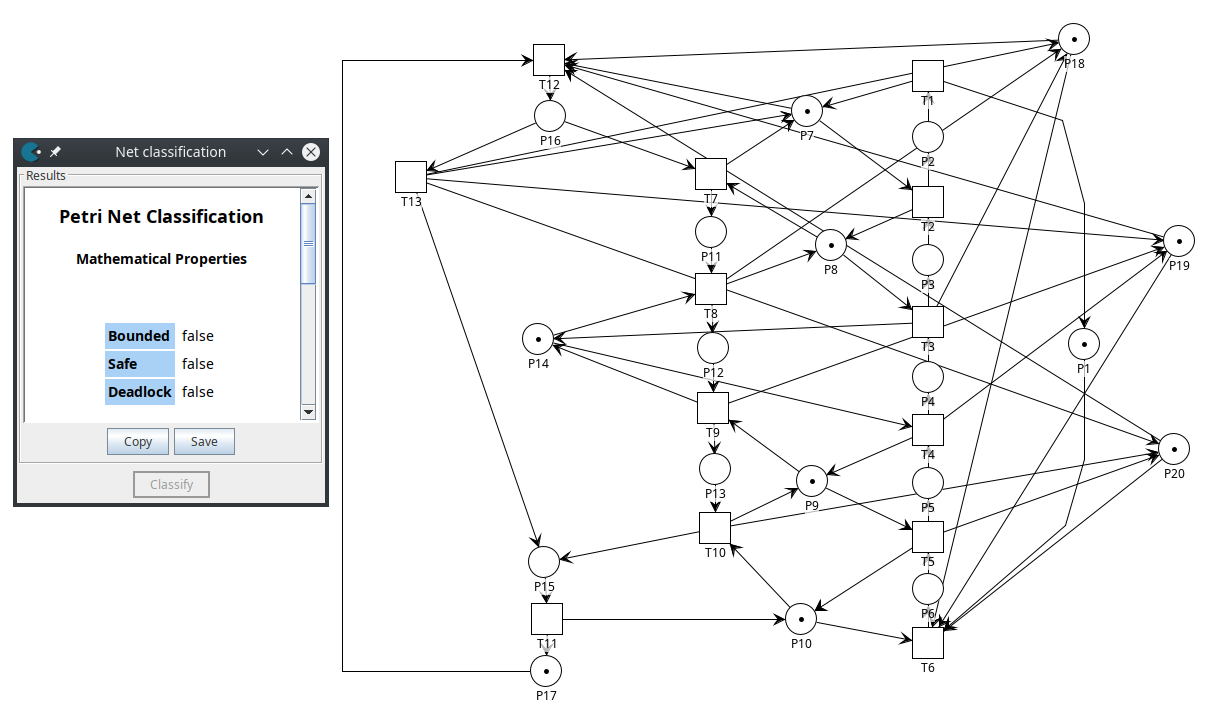
\includegraphics[scale=0.5]{Figures/algoritmo3/POP4.png}
	\caption{ Subred derecha POPN controlada.}
	\label{fig:popnreddercontrolada}
 \end{figure}
\bigskip

\begin{table}[H]
    \centering
    \begin{tabular}{|c|c|P{2.2cm}|P{2.2cm}|c|}
    \hline
    \textbf{Supervisor} & \textbf{Marcado} & \textbf{Transiciones input} & \textbf{Transiciones output} & \textbf{Bad Siphon Controlado}  \\  \hline
    $P_{27}$ & 1 & \{$T_{7}, T_{15}, T_{19}$\} & \{$T_{12}, T_{17}$\} & \{$P_1,P_{7},P_{9},P_{12}$\} \\ 
    \hline
    \end{tabular}
    \label{tab:popnizq}
    \caption{Supervisores: RdP POPN (L).}
    \end{table}

\begin{figure}[H]
	\centering
	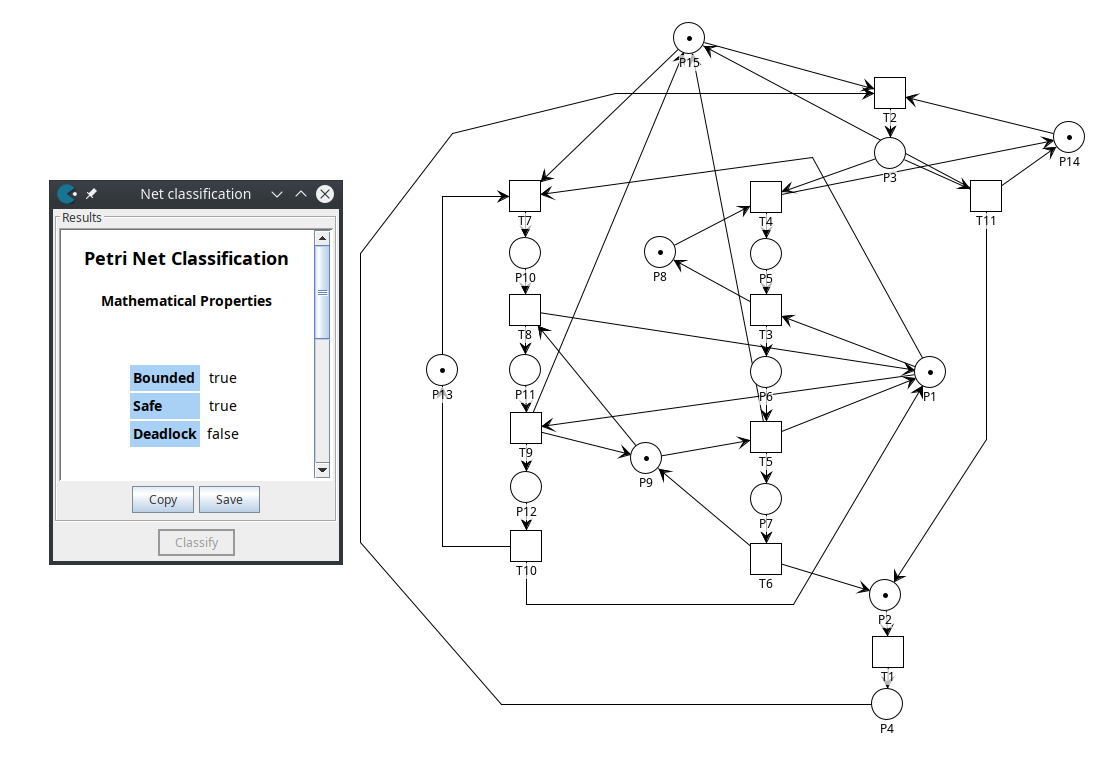
\includegraphics[scale=0.5]{Figures/algoritmo3/POP5.png}
	\caption{Subred izquierda POPN controlada.}
	\label{fig:popnredizqcontrolada}
 \end{figure}
 
 \paragraph{Control red original}
 \hfill \break
Al contemplar el conflicto en el análisis de cada subred, la unión de las soluciones individuales permiten resolver el deadlock de la red completa, sin necesidad de realizar otro análisis.\\
\bigskip

\begin{figure}[H]
	\centering
	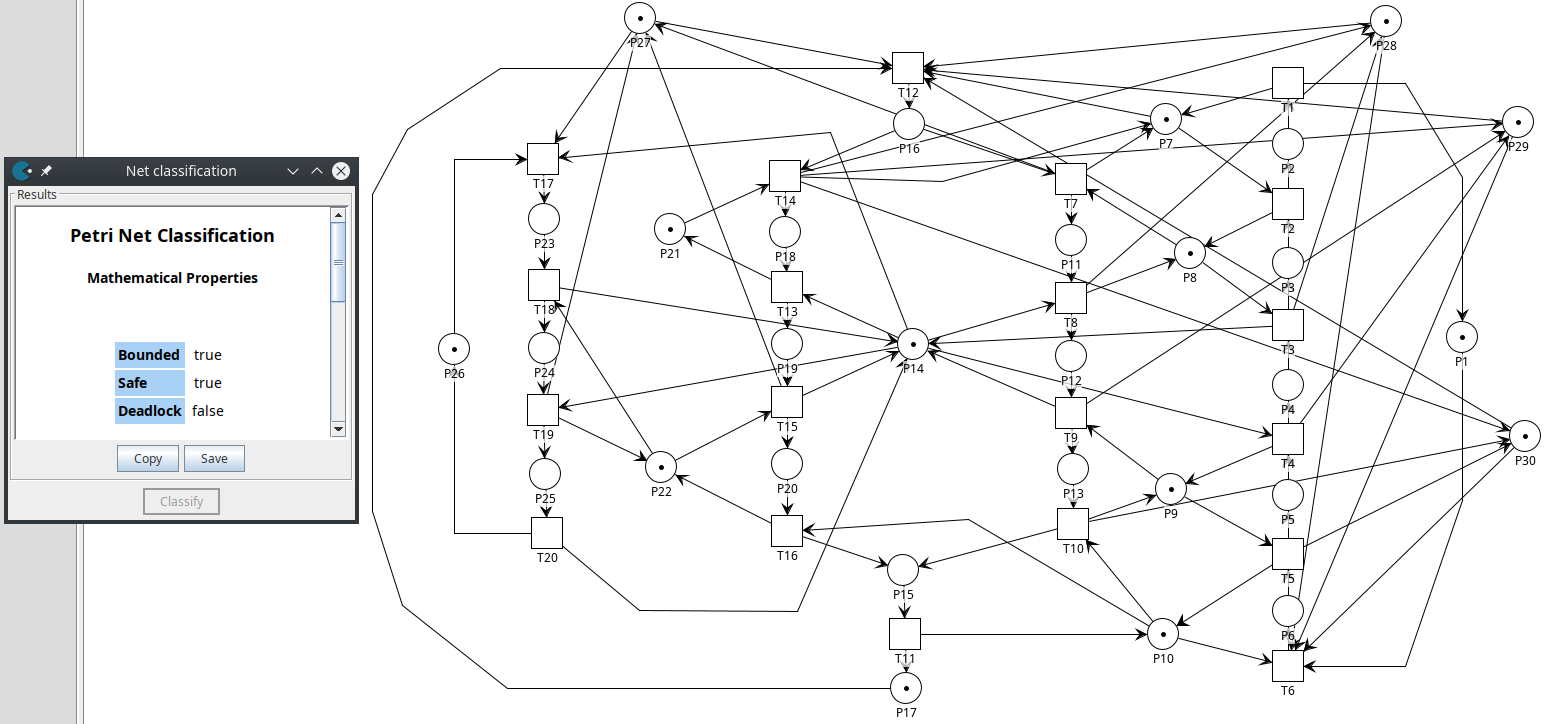
\includegraphics[width=\textwidth]{Figures/algoritmo3/POP6.png}
	\caption{RdP POPN controlada.}
	\label{fig:popncontrolada}
 \end{figure}
\bigskip

\subsubsection{Caso Guanjun} \label{sec:guanjun}
Esta red modela la ejecución concurrente de procesos de trabajo en FMS que describe el comportamiento de 2 subredes relacionadas por dos recursos, en caso de llevar una mala gestión de estos la red terminará en deadlock.
\bigskip

\paragraph{Características generales}
\begin{itemize}
    \item Presenta conflicto entre T-invariantes.
    \item Los recursos R1-R5 están representados por las plazas $\{P_{11}, P_{12}, P_{14}, P_{15}, P_{18}\}$, con $P_{14}$ y $P_{15}$ compartidas por las tres subredes.
\end{itemize}

\subparagraph{Análisis estructural}
\hfill
\begin{figure}[H]
	\centering
	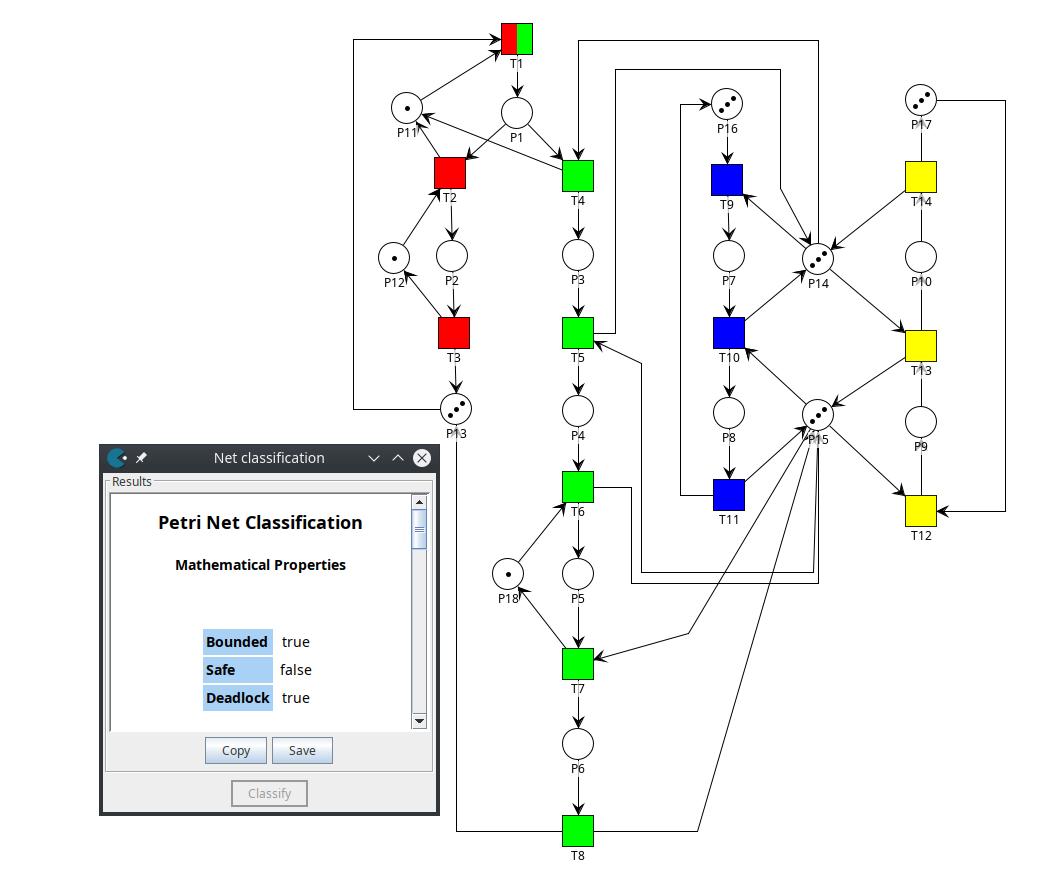
\includegraphics[scale=0.5]{Figures/algoritmo3/Guanjun1.png}
	\caption[RdP Guanjun \ y sus T-invariantes.]{RdP Guanjun \footnotemark \ y sus T-invariantes.}
	\label{fig:guanjuntinvariantes}
 \end{figure} \footnotetext{Figura adaptada del paper publicado por \textit{G. Liu, C. Jiang and M. Zhou} \cite{paperguanjun}. }
 
En la figura \ref{fig:guanjuntinvariantes}, la plaza $P_1$ forma parte de un conflicto permitiendo la ejecución de un subcircuito de la red u otro, pudiendo seguir dos T-invariantes diferentes (rojo o verde en este caso). Pero en este caso, a diferencia de los anteriores, al ejecutar el algoritmo mencionado desde el punto 1-4 por primera vez sobre la red completa, permite encontrar los supervisores que resuelven el deadlock sin necesidad de subdividir la red (es decir, ejecutar el paso 5). Dado que el token independientemente del T-invariante que siga siempre vuelve a los supervisores, como se puede observar en la figura \ref{fig:guanjuncontrolada}.\\

\subparagraph{Red controlada}
\hfill \break
Una vez ejecutado el algoritmo, se obtienen la plaza y los arcos a agregar para controlar la red, solucionando el problema de deadlock.\\

\begin{table}[H]
    \centering
    \begin{tabular}{|c|c|P{2.5cm}|P{2.2cm}|c|}
    \hline
    \textbf{Supervisor} & \textbf{Marcado} & \textbf{Transiciones input} & \textbf{Transiciones output} & \textbf{Bad Siphon Controlado}  \\  \hline
    $P_{19}$ & 6 & \{$T_{2}, T_{7}, T_{10}, T_{13}$\} & \{$T_{1}, T_{9}, T_{12}$\} & \{$P_6,P_{8},P_{10},P_{14},P_{15},P_{18}$\} \\ 
    \hline
    $P_{20}$ & 5 & \{$T_{2}, T_{5}, T_{10}, T_{13}$\} & \{$T_{1}, T_{9}, T_{12}$\} & \{$P_4,P_{6},P_{8},P_{10},P_{14},P_{15}$\} \\ 
    \hline
    \end{tabular}
    \label{tab:guanjun}
    \caption{Supervisores: RdP Guanjun.}
    \end{table}
\bigskip

\begin{figure}[H]
	\centering
	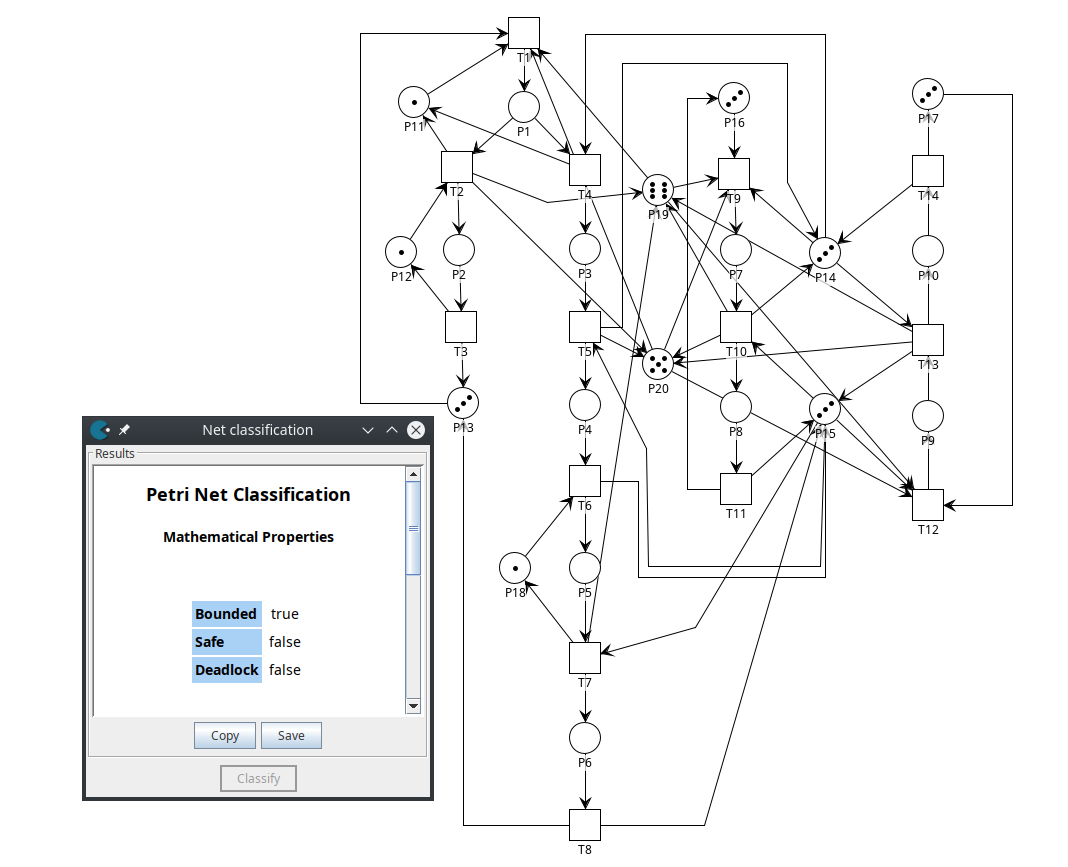
\includegraphics[scale=0.5]{Figures/algoritmo3/Guanjun2.png}
	\caption{RdP Guanjun controlada.}
	\label{fig:guanjuncontrolada}
 \end{figure}
\bigskip

\subsubsection{Caso Hospital} \label{sub:Hospital}
En esta red se modela el caso de un hospital. Los elementos del mismo considerados por esta serán la recepción (PW) donde se reciben los pacientes y se realiza el trabajo administrativo, la sala de consulta (CR) donde un médico da el diagnóstico a los pacientes, la sala de cirugía (S) donde se realizan las cirugías y el médico (D) que realizará todos estos procedimientos.\\
Además se tendrá las siguientes consideraciones:

\begin{itemize}
    \item La persona que trabaja en la recepción y el médico podrían atender a una persona por vez.
    \item Tanto en la sala de consulta como en la sala de cirugía, solo un paciente a la vez podría ser tratado, es decir, podemos decir que su capacidad máxima es igual a uno.
    \item Si queremos que el hospital funcione en buenas condiciones, los pacientes y el personal del hospital deben respetar algunos protocolos:
        \begin{itemize}
            \item El hospital tiene dos entradas: una normal y otra de emergencia.
                \begin{itemize}
                    \item Los pacientes que llegan a la entrada normal (IN1) tienen que ir primero a la recepción (PW) para realizar el papeleo. Dependiendo de los problemas que tengan los pacientes, pueden ser enviados a la sala de consulta (CR) o a la sala de cirugía (S). Después de que los pacientes terminan con cualquiera de estos, van a ver al médico (Dr) para obtener el certificado de liberación. Con todas estas cosas hechas, los pacientes pueden salir del hospital (OUT1).
                    \item El hospital tiene otra entrada (IN2): para los casos de emergencia. Los pacientes que llegaron a IN2, son revisados por el médico (D), y luego enviados a la sala de cirugía. Desde el quirófano tienen que llenar los papeles, por lo que primero deben ir a PW y luego pueden irse a casa(OUT2). 
                    \bigskip
                    
                    \begin{figure}[H]
                	\centering
                	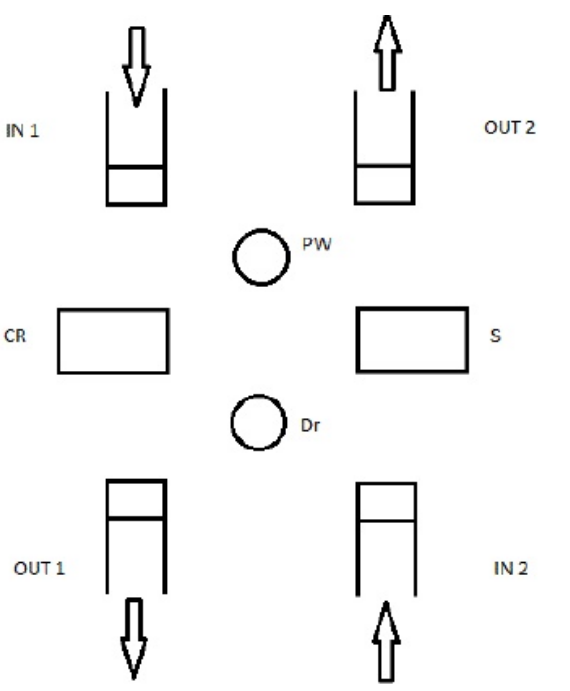
\includegraphics[scale=0.6]{Figures/algoritmo3/hospitalmodelado.png}
                	\caption[Modelado de partes del sistema Hospital]{Modelado de partes del sistema Hospital. \footnotemark .}
                	\label{fig:onosdistribuido}
                 \end{figure}
                \end{itemize}
        \end{itemize}
\end{itemize}

\footnotetext{Figura adaptada del paper publicado por \textit{A. Timotei y J. Colom}\cite{paperhospital} .}

\bigskip

\newpage
\paragraph{Características generales}
\hfill
\begin{itemize}
    \item Presenta conflictos entre T-invariantes.
    \item La sala de consulta está representada por la plaza $P_{11}$, la recepción por la $P_8$, la sala de cirugía por la $P_9$ y doctores por la $P_{10}$.
\end{itemize}

\subparagraph{Análisis estructural}
\hfill
\begin{figure}[H]
	\centering
	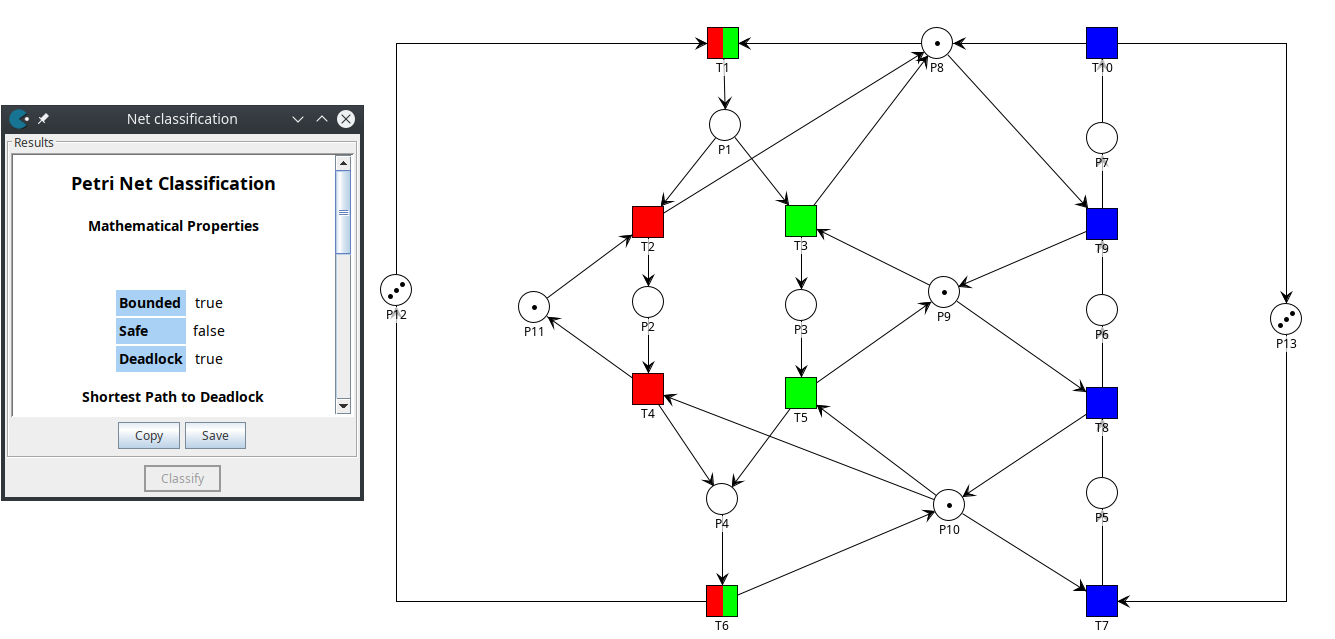
\includegraphics[scale=0.4]{Figures/algoritmo3/Hospital1.png}
	\caption[RdP Hospital y sus T-invariantes.]{RdP Hospital \footnotemark \ y sus T-invariantes.}
	\label{fig:onosdistribuido}
 \end{figure} \footnotetext{Figura adaptada del paper publicado por \textit{A. Timotei y J. Colom} \cite{paperhospital} .}

En este caso particular de red en el que la plaza $P_1$ forma parte de un conflicto permitiendo la ejecución de un subcircuito de la red u otro, pudiendo seguir dos T-invariantes diferentes (rojo o verde en este caso).
Por esto fue necesario ejecutar el algoritmo de forma completa (5 pasos).\\

En un principio se buscó dividir la red preservando el conflicto en las subredes individualmente (como en los casos previos) pero las subredes resultantes no presentaban deadlock (figura \ref{fig:hospitalsubredderechaconflicto}).

\hfill
\begin{figure}[H]
	\centering
	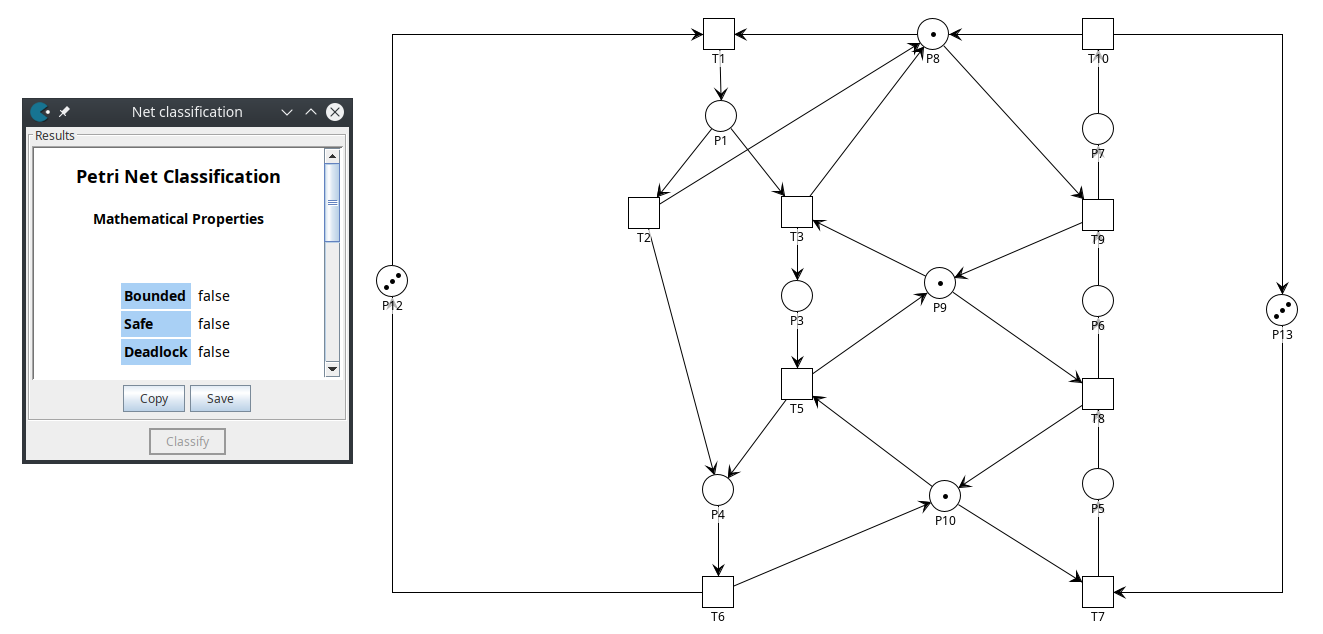
\includegraphics[scale=0.4]{Figures/algoritmo3/Hospital2.png}
	\caption{Subred derecha Hospital contemplando el conflicto.}
	\label{fig:hospitalsubredderechaconflicto}
 \end{figure}

Por este motivo, se optó por dividir la red contemplando en cada una de las subredes sólo uno de los caminos del conflicto y el otro T-invariante presente en la red; obteniendo dos subredes.

\subparagraph{Subred derecha}
\hfill
\begin{figure}[H]
	\centering
	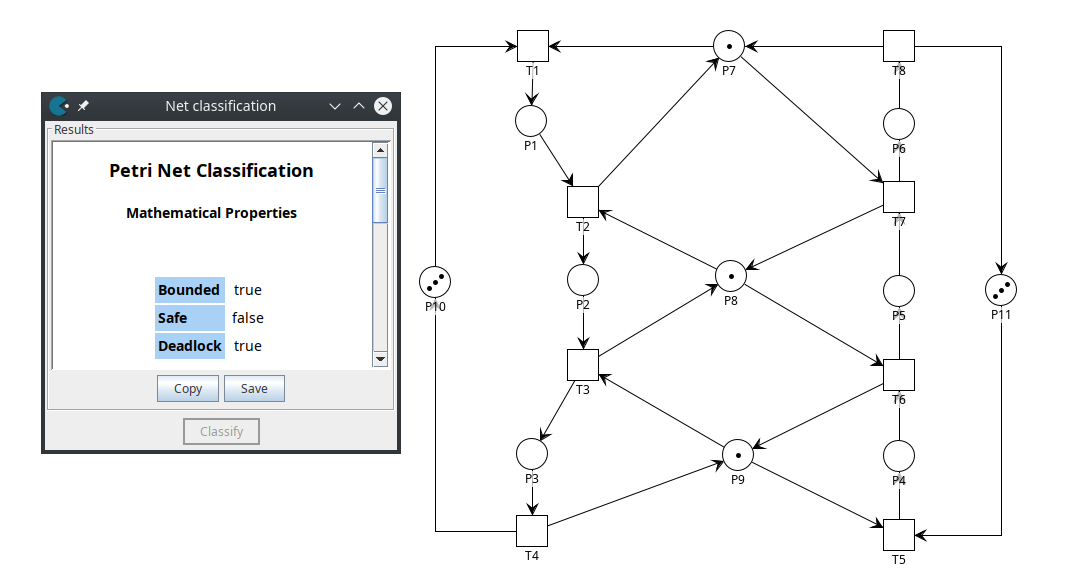
\includegraphics[scale=0.5]{Figures/algoritmo3/Hospital3.png}
	\caption{RdP Hospital preservando lado derecho del conflicto.}
	\label{fig:ladoderechoconflicto}
 \end{figure}

\subparagraph{Subred izquierda}
\hfill
\begin{figure}[H]
	\centering
		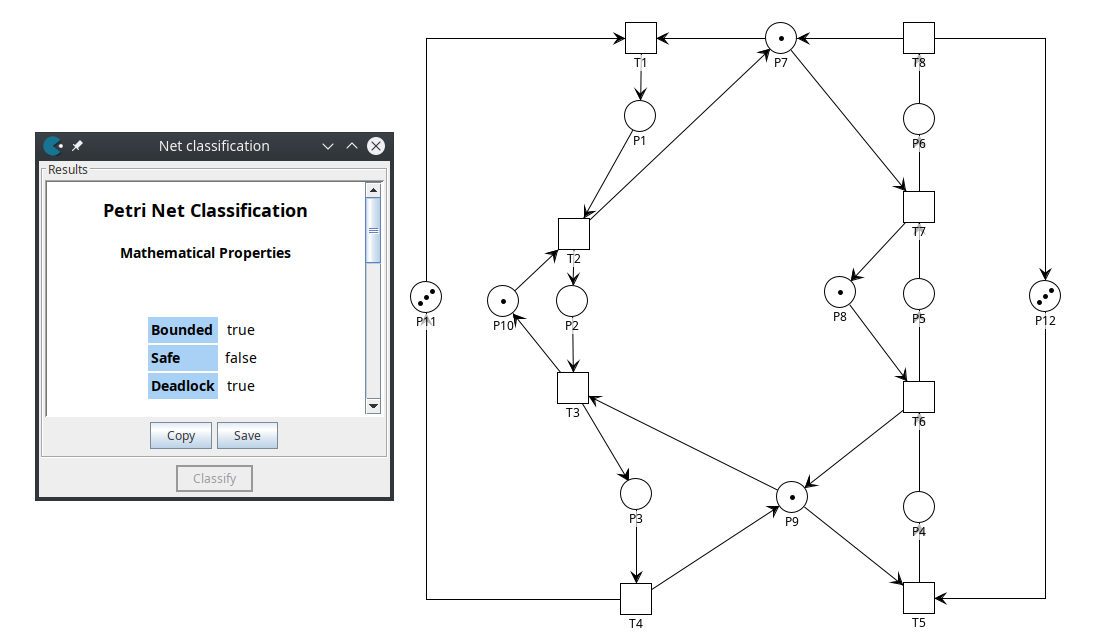
\includegraphics[scale=0.5]{Figures/algoritmo3/Hospital4.png}
	\caption{RdP Hospital preservando lado izquierdo del conflicto.}
	\label{fig:ladoizquierdoconflicto}
 \end{figure}

\newpage
\subparagraph{Control subredes}
\hfill \break
Se ejecutaron los primeros 4 ítems del algoritmo obteniendo los supervisores correspondientes, resolviendo el deadlock en cada subred.
\bigskip

\begin{table}[H]
    \centering
    \begin{tabular}{|c|c|P{2.2cm}|P{2.2cm}|c|}
    \hline
    \textbf{Supervisor} & \textbf{Marcado} & \textbf{Transiciones input} & \textbf{Transiciones output} & \textbf{Bad Siphon Controlado}  \\  \hline
    $P_{14}$ & 3 & \{$T_{3}, T_{7}$\} & \{$T_{1}, T_{5}$\} & \{$P_2, P_{7}, P_{6}, P_{7}, P_{8}$\} \\ 
    \hline
    \end{tabular}
    \caption{Supervisores: RdP Hospital (L).}
    \label{tab:Hospital-SubL}
\end{table}
\bigskip

\begin{figure}[H]
	\centering
		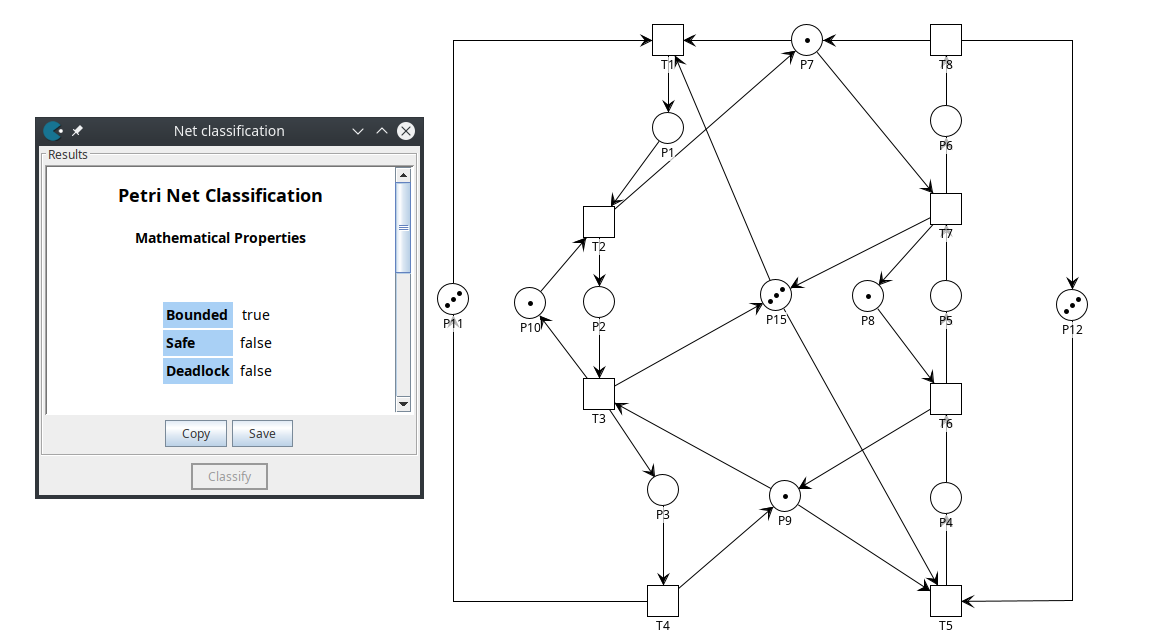
\includegraphics[width=\textwidth]{Figures/algoritmo3/Hospital5.png}
	\caption{Control RdP Hospital preservando lado izquierdo del conflicto.}
	\label{fig:ladoizquierdoconflictocontrol}
 \end{figure}
\bigskip

\begin{table}[H]
    \centering
    \begin{tabular}{|c|c|P{2.2cm}|P{2.2cm}|c|}
    \hline
    \textbf{Supervisor} & \textbf{Marcado} & \textbf{Transiciones input} & \textbf{Transiciones output} & \textbf{Bad Siphon Controlado}  \\  \hline
    $P_{14}$ & 1 & \{$T_{2}, T_{3}, T_9$\} & \{$T_{1}, T_{7}$\} & \{$P_2, P_{6}, P_{7}, P_{8}$\} \\ 
    \hline
    $P_{15}$ & 2 & \{$T_{4}, T_{5}, T_9$\} & \{$T_{1}, T_{7}$\} & \{$P_{3},P_{6},P_{7},P_{8}, P_{9}$\} \\ 
    \hline
    $P_{16}$ & 1 & \{$T_{2}, T_{5}, T_8$\} & \{$T_{1}, T_{7}$\} & \{$P_{3},P_{5},P_{8},P_{9}$\} \\ 
    \hline
    \end{tabular}
    \caption{Supervisores: RdP Hospital (R).}
    \label{tab:Hospital-SubR}
\end{table}

\begin{figure}[H]
	\centering
		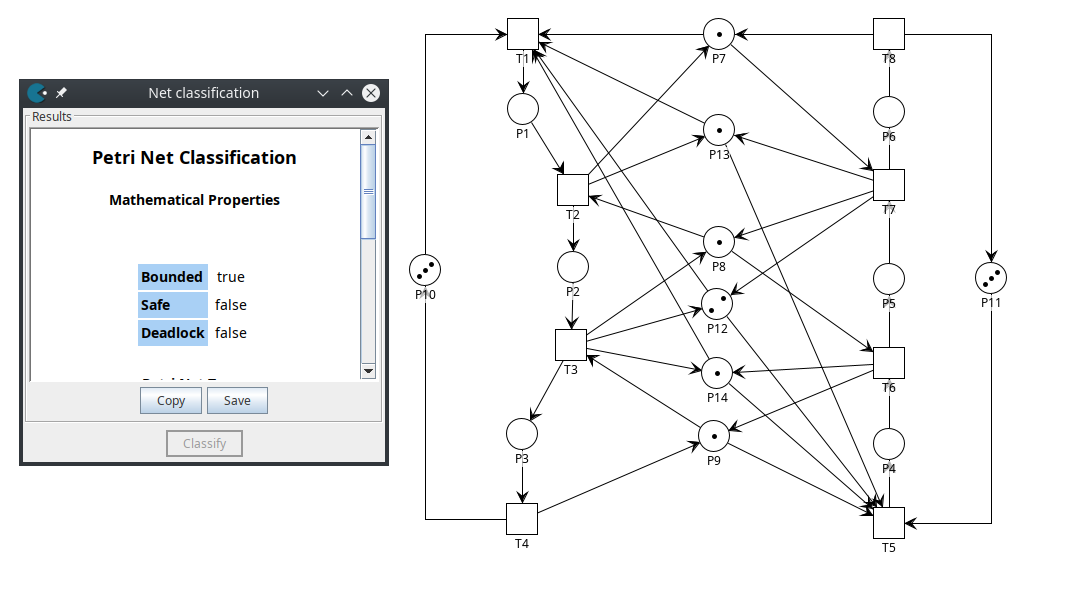
\includegraphics[scale=0.45]{Figures/algoritmo3/Hospital6.png}
	\caption{Control RdP Hospital preservando lado derecho del conflicto.}
	\label{fig:ladoderechoconflictocontrol}
 \end{figure}

\subparagraph{Control red original}
\hfill \break
Al unir las soluciones individuales la red seguía presentando deadlock, lo que sucedió en este caso particular es que al unir ambas subredes entraron en juego nuevos supervisores que formaban parte del control de las plazas pertenecientes al otro \break T-invariante en conflicto. Por este motivo en caso de tomarse el camino ajeno al supervisor, la transición en conflicto debería devolver el token al mismo. Esto se puede visualizar en el caso de los supervisores representados por las plaza $P_{14}$ y $P_{16}$, dado que los mismos pertenecen al control de la subred derecha, por ende no están presentes en el control de la subred izquierda; de esta manera si la red al ejecutarse toma el camino del T-invariante izquierdo, la transición $T_2$ (que es la que da inicio a este camino) debe devolver el token consumido a estos supervisores no contemplados, conservando de esta manera la vivacidad de la red.\\
Además, se da el caso en el que las subredes individualmente presentan supervisores en común, por lo que el marcado del mismo (al momento de la unión) debía colocarse con el menor de ellos.\\
Para solucionar lo anterior se realizó lo mencionado en el punto 5.b (sección \ref{sec:desarrollov3}) del algoritmo.

\begin{figure}[H]
	\centering
		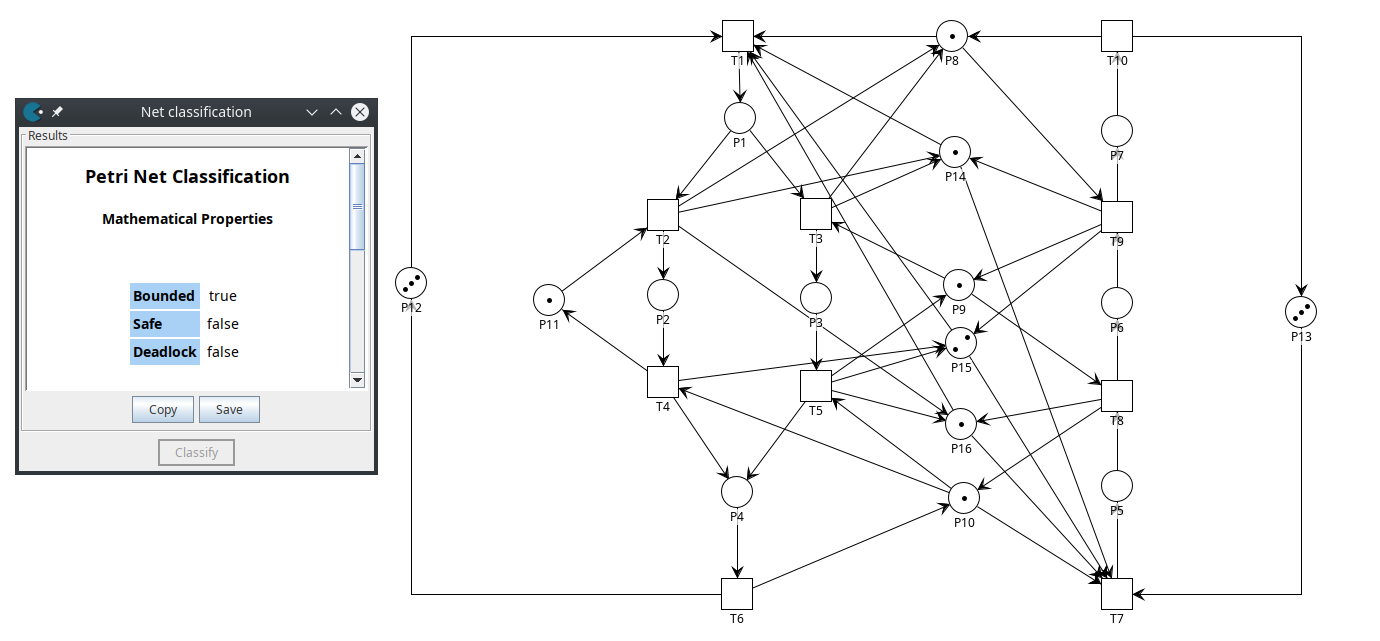
\includegraphics[scale=0.4]{Figures/algoritmo3/Hospital7.png}
	\caption{RdP Hospital controlada.}
	\label{fig:hospitalcontrolada}
 \end{figure}

\subsubsection{Caso Huang}
Esta red modela la ejecución concurrente de procesos de trabajo en FMS, representando un sistema donde se ejecutan tres tipos de procesos de trabajo.\\
En la red existen plazas que simulan la disponibilidad de recursos (4) y un control incorrecto de estos en la ejecución de los procesos de trabajo, puede conducir a situaciones de deadlock.\\

\paragraph{Características generales}
\begin{itemize}
    \item Presenta un conflicto entre T-invariantes. 
    \item Los recursos R1-R4 están representados por las plazas $\{P_6, P_7, P_{12}, P_{13}\}$
    \end{itemize}
\bigskip

\subparagraph{Análisis estructural}
\hfill
\begin{figure}[H]
	\centering
	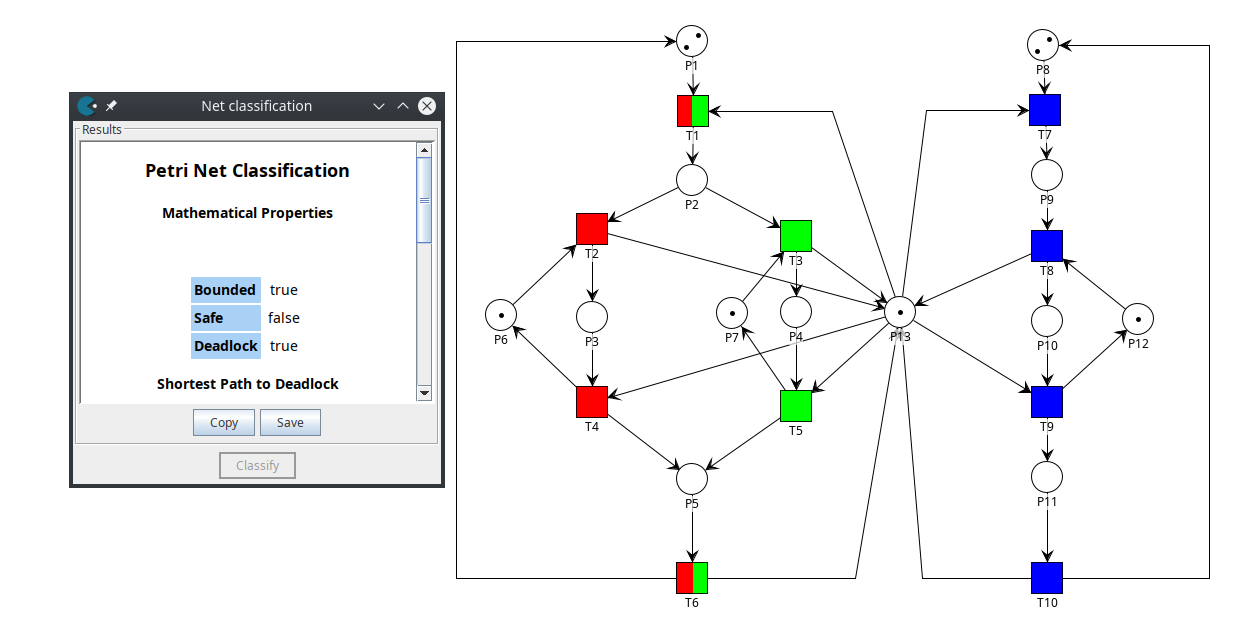
\includegraphics[width=\textwidth]{Figures/algoritmo3/Huang1.png}
	\caption[RdP Huang y sus T-invariantes.]{RdP Huang \footnotemark \ y sus T-invariantes.}
	\label{fig:huang_T-invariantes}
 \end{figure} \footnotetext{Figura adaptada del paper publicado por \textit{Huang} et al. \cite{paperhuang} .}
\bigskip

En la figura \ref{fig:huang_T-invariantes}, la plaza $P_2$ forma parte de un conflicto permitiendo la ejecución de un subcircuito de la red u otro, pudiendo seguir dos T-invariantes diferentes (rojo o verde, en este caso).\\
Dado que los primeros 4 pasos del algoritmo no lograron alcanzar una red libre de deadlock, fue necesario ejecutarlo de forma completa, es decir, incluyendo el paso 5, contemplando la división de la red.
De la división resultaron dos subredes, preservando el recurso compartido ($P_{13}$) en cada una de ellas.

\subparagraph{Subred izquierda}
\hfill \break
Esta subred no fue necesario controlarla mediante un supervisor dado que no presenta deadlock.

\begin{figure}[H]
	\centering
	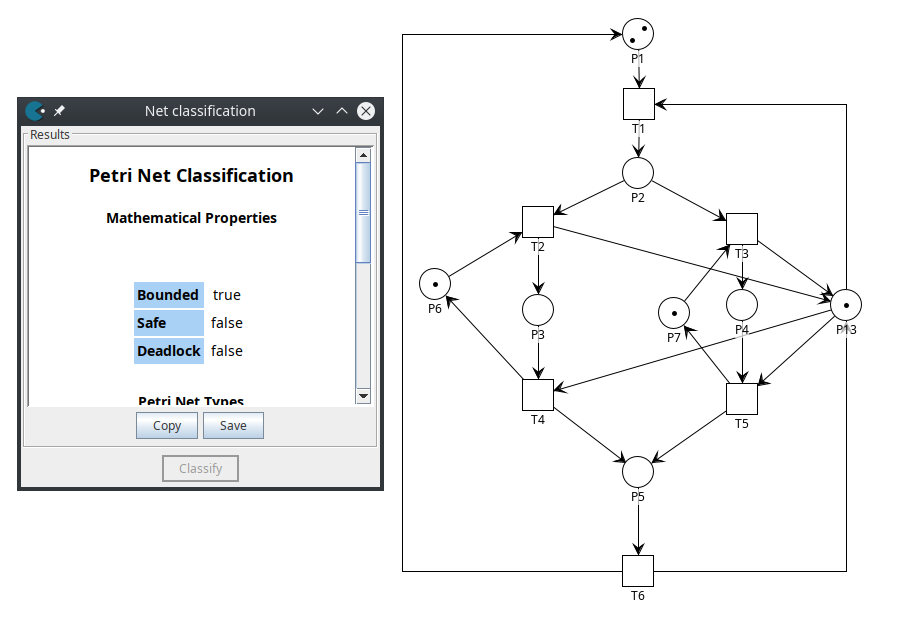
\includegraphics[scale=0.5]{Figures/algoritmo3/Huang2.png}
	\caption{Subred izquierda Huang.}
	\label{fig:Huang_subredizq}
 \end{figure}
 
 \subparagraph{Subred derecha}
\hfill \break
Esta subred no fue necesario controlarla mediante un supervisor dado que no presenta deadlock.

\begin{figure}[H]
	\centering
	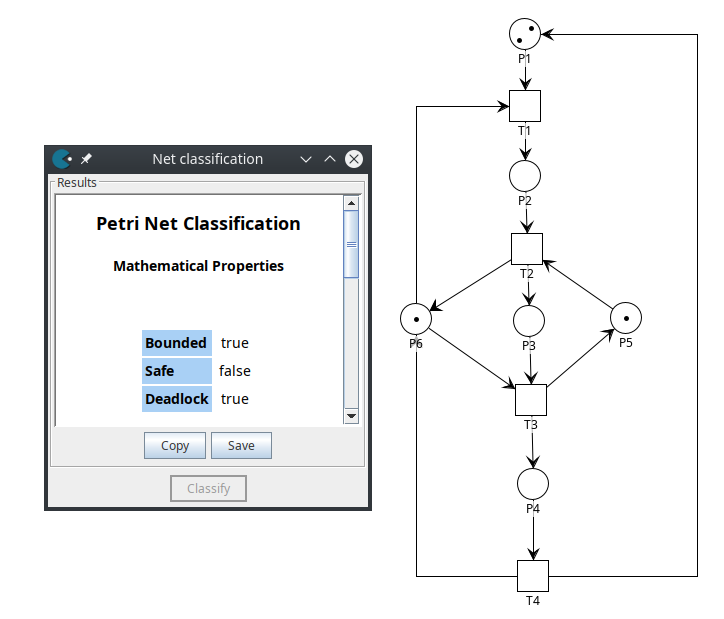
\includegraphics[scale=0.5]{Figures/algoritmo3/Huang3.png}
	\caption{Subred derecha Huang.}
	\label{fig:Huang_subredder}
 \end{figure}

\subparagraph{Control subredes}
\hfill \break
Una vez ejecutado el algoritmo (4 primeros pasos) sobre la subred derecha, se obtuvo el supervisor a agregar para su control, resolviendo así el problema de deadlock.

 \begin{figure}[H]
	\centering
	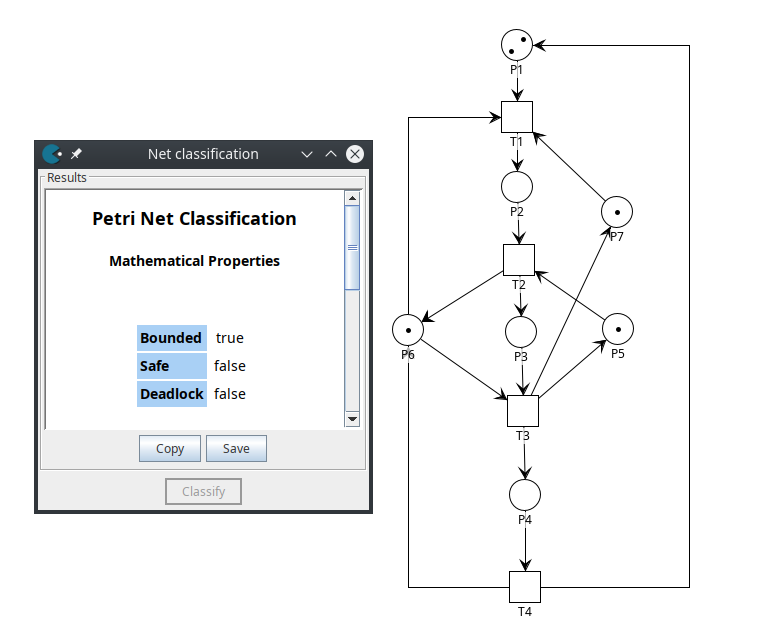
\includegraphics[scale=0.5]{Figures/algoritmo3/Huang4.png}
	\caption{Subred derecha Huang controlada.}
	\label{fig:subredder_huang_controlada.}
 \end{figure}

\subparagraph{Red controlada}
\hfill \break
Al haber contemplado en ambas subredes el recurso compartido, cuando se las integró en la red completa no fue necesario agregar otro tipo de arcos para mantener el deadlock false.

\begin{table}[H]
    \small
    \centering
    \begin{tabular}{|c|c|P{2.2cm}|P{2.2cm}|c|}
    \hline
    \textbf{Supervisor} & \textbf{Marcado} & \textbf{Transiciones input} & \textbf{Transiciones output} & \textbf{Bad Siphon Controlado}  \\  \hline
    $P_{14}$ & 1 & \{$T_{9}$\} & \{$T_{7}$\} & \{$P_{11}, P_{12}, P_{13}$\} \\ 
    \hline
    \end{tabular}
    \caption{Supervisores: RdP Huang.}
    \label{tab:Huang-v3}
\end{table}

 \begin{figure}[H]
	\centering
	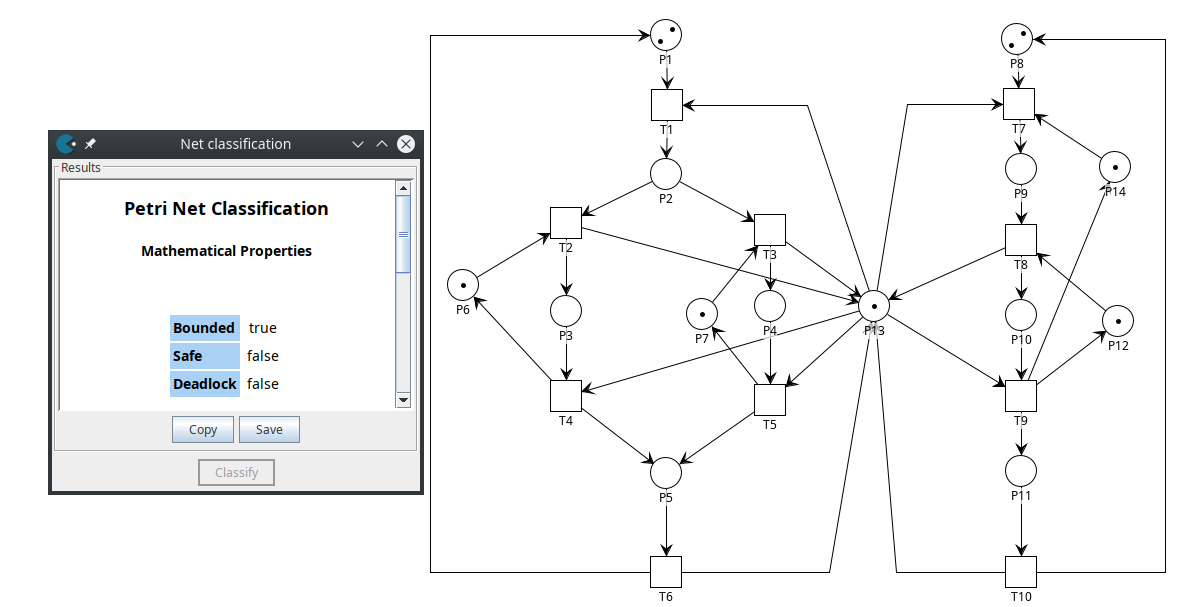
\includegraphics[scale=0.46]{Figures/algoritmo3/Huang5.png}
	\caption{RdP Huang controlada.}
	\label{fig:huang_controlada}
 \end{figure}
 \bigskip

\subsubsection{Caso MFC}
En esta red se modela un FMS. El mismo consta de un conjunto de estaciones de trabajo que comparten una serie de recursos como: 
\begin{itemize}
    \item Robots R1, R2 y R3 , donde cada uno puede contener un producto a la vez.
    \item Máquinas M1,M2,M3 y M4 , donde cada una puede procesar dos productos a la vez.
    \item Accesorios de vehículos guiados automáticamente (AGV).
    \item Buffers tanto de carga I1 e I2 , como de descarga O1 y O2.
\end{itemize}

\noindent Con los cuales lleva a cabo la producción de dos tipos de productos: $parte_1$ y $parte_2$.
\bigskip

\begin{figure}[H]
	\centering
	\includegraphics[scale=0.45]{Figures/algoritmo3/mfcmodelado.png}
	\caption[Modelado de partes del sistema MFC.]{Modelado de partes del sistema MFC\footnotemark.}
	\label{fig:sistema_mfc}
 \end{figure} \footnotetext{Figura adaptada del paper publicador por \textit{Mowafak H. Abdul-Hussin} \cite{papermfc} .}
\bigskip

\paragraph{Características generales}
\begin{itemize}
    \item Las máquinas M1,M2,M3,M4 están representadas por las plazas $\{P_{12}, P_{14}, P_{18}, P_{19}\}$
    \item Los robots R1,R2,R3 están representados por las plazas $\{P_{11}, P_{13}, P_{15}\}$
    \item La línea de producción de las ${parte_1}$ está representada por las plazas $\{P_1-P_5\}$, mientras que las ${parte_2}$ por las plazas $\{P_6-P_{10}\}$.
\end{itemize}

\paragraph{Análisis estructural}
\hfill
\begin{figure}[H]
	\centering
	\includegraphics[scale=0.45]{Figures/algoritmo3/MFC1.png}
	\caption[RdP MFC \ y sus T-invariantes.]{RdP MFC \footnotemark \ y sus T-invariantes.}
	\label{fig:mfc_T-invariantes} 
 \end{figure} \footnotetext{Figura adaptada del paper publicador por \textit{Mowafak H. Abdul-Hussin} \cite{papermfc} .}
 
En la figura \ref{fig:mfc_T-invariantes}, se representan los T-invariantes, en rojo y verde. \\
Sobre esta red se ejecutaron los primeros 4 pasos del algoritmo, permitiendo encontrar el supervisor que resuelva el deadlock sin necesidad de subdividirla (paso 5); incluso realizar esta acción carecía de sentido dado que los T-invariantes por separado no representan el comportamiento de la red en su totalidad.\\

\paragraph{Red controlada}
\hfill \break
Una vez incorporado el supervisor a la red, es decir, las plazas y arcos determinados por el algoritmo, se logra su control resolviendo así el problema de deadlock.

\begin{table}[H]
    \centering
    \begin{tabular}{|c|c|P{2.2cm}|P{2.2cm}|c|}
    \hline
    \textbf{Supervisor} & \textbf{Marcado} & \textbf{Transiciones input} & \textbf{Transiciones output} & \textbf{Bad Siphon Controlado}  \\  \hline
    $P_{21}$ & 2 & \{$T_{2}, T_{11}$\} & \{$T_{1}, T_{7}$\} & \{$P_{2},P_{10},P_{11}, P_{12}$\} \\ 
    \hline
    $P_{22}$ & 2 & \{$T_{3}, T_{10}$\} & \{$T_{1}, T_{7}$\} & \{$P_3, P_{9}, P_{12}, P_{13}$\} \\ 
    \hline
    $P_{23}$ & 2 & \{$T_{4}, T_{9}$\} & \{$T_{1}, T_{7}$\} & \{$P_{4},P_{8},P_{13},P_{14}$\} \\ 
    \hline
    \end{tabular}
    \caption{Supervisores: RdP MFC.}
    \label{tab:MFC-v3}
\end{table}

\begin{figure}[H]
	\centering
	\includegraphics[scale=0.5]{Figures/algoritmo3/MFC2.png}
	\caption{RdP MFC controlada.}
	\label{fig:mfc_controlada}
 \end{figure}
\bigskip

\subsubsection{Caso Portugal} \label{sub:portugal}
Esta red modela la ejecución concurrente de procesos de trabajo en FMS, representando un sistema donde se ejecutan cuatro tipos de procesos de trabajo con estaciones de trabajo (4) idénticas, con dos recursos compartidos por todas, en caso de llevar una mala gestión de estos la red terminará en deadlock.

\paragraph{Características generales}
\begin{itemize}
    \item En este caso particular la red es simétrica, pudiéndose dividir en 4 partes iguales, todas manteniendo el deadlock.
    \item Se trabajó sobre una de estas porciones de red, extendiendo luego la solución a las restantes partes.
\end{itemize}
\bigskip

\newpage
\paragraph{Análisis estructural}
\hfill

\begin{figure}[H]
	\centering
	\includegraphics[scale= 0.45]{Figures/algoritmo3/Portugal1.png}
	\caption[RdP Portugal y sus T-invariantes.]{RdP Portugal \footnotemark \ y sus T-invariantes.}
	\label{fig:portugal_T-invariantes}
 \end{figure} \footnotetext{Figura adaptada del paper publicado por \textit{S. Wang} et al. \cite{paperportugal} .}


De acuerdo con las características de la red, se trabajó sobre una de las cuatro subredes resultantes mediante el algoritmo (pasos 1 al 4), obteniendo el supervisor que controla el problema del deadlock presente en ese ¼ de red.\\
Pudiéndose aplicar la misma solución a todas las restantes subredes, dada su simetría.\\
Al momento de unirlas con sus respectivas soluciones, hay que tener en cuenta que el recurso compartido está afectando todos los T-invariantes, por lo que se deben aplicar los arcos que componen a cada supervisor ajeno.\\

\subparagraph{¼ de red}
\hfill

\begin{figure}[H]
	\centering
	\includegraphics[scale=0.6]{Figures/algoritmo3/Portugal2.png}
	\caption{Porción de la RdP Portugal.}
	\label{fig:cuartodered_portugal}
 \end{figure}
\subparagraph{Control ¼ de la red}
\hfill \break
Una vez ejecutado el algoritmo (4 primeros ítems) sobre ¼ de la red el problema de deadlock fue solucionado.

\begin{table}[H]
    \centering
    \begin{tabular}{|c|c|P{2.2cm}|P{2.2cm}|c|}
    \hline
    \textbf{Supervisor} & \textbf{Marcado} & \textbf{Transiciones input} & \textbf{Transiciones output} & \textbf{Bad Siphon Controlado}  \\  \hline
    $P_{9}$ & 2 & \{$T_{2}, T_{5}$\} & \{$T_{1}, T_{4}$\} & \{$P_3, P_{6}, P_{7}, P_{8}$\} \\ 
    \hline
    \end{tabular}
    \caption{Supervisores: RdP Portugal.}
    \label{tab:Portugal-v3}
\end{table}

\begin{figure}[H]
	\centering
	\includegraphics[scale=0.55]{Figures/algoritmo3/Portugal3.png}
	\caption{Porción de la RdP Portugal controlada.}
	\label{fig:cuartodered_portugalcontrolada}
 \end{figure}

\subparagraph{Control ½ de la red}
\hfill \break
Realizando lo mencionado en el análisis estructural se decidió unificar las soluciones de dos cuartos de la red y como se observa en la figura \ref{fig:mitadred_portugalcontrolada} la subred no presenta deadlock.\\
Lo mismo ocurriría si se unifican las 4 partes pero con el objetivo de lograr una mejor visualización del control,  se optó por no desarrollarla en el presente informe.

\begin{figure}[H]
	\centering
	\includegraphics[scale=0.45]{Figures/algoritmo3/Portugal4.png}
	\caption{Mitad de la RdP Portugal controlada.}
	\label{fig:mitadred_portugalcontrolada}
 \end{figure}
\bigskip

\subsubsection{Caso Zhao}
Esta red modela la ejecución concurrente de procesos de trabajo en FMS que describe el comportamiento de 3 subredes relacionadas por tres recursos, en caso de llevar una mala gestión de estos la red terminará en deadlock.

\paragraph{Características generales}
\begin{itemize}
    \item Presenta conflictos entre T-invariantes.
    \item Los recursos R1-R3 están representados por las plazas $\{P_{15}, P_{16}, P_{17}\}$. \\
\end{itemize}
\bigskip

\subparagraph{Análisis estructural}
\hfill \break
\begin{figure}[H]
	\centering
	\includegraphics[width=\textwidth]{Figures/algoritmo3/Zhao1.png}
	\caption[RdP Zhao y sus T-invariantes.]{RdP Zhao \footnotemark \ y sus T-invariantes.}
	\label{fig:zhao_T-invariantes}
 \end{figure} \footnotetext{Figura adaptada del paper publicado por \textit{Mi Zhao} et al. \cite{paperzhao} .}
 
En la figura \ref{fig:zhao_T-invariantes} \footnote{En esta RdP fue modificado el peso de los arcos reduciéndolos a uno (1) para adaptarla al tipo de red que admite el algoritmo.}, las plazas $P_1$ y $P_5$ forma parte (cada una) de un conflicto permitiendo su disparo la ejecución de un subcircuito de la red u otro, pudiendo seguir dos T-invariantes diferentes (rojo o verde en este caso). Pero en este caso, al igual que en la red Guanjun (sección \ref{sec:guanjun}), al ejecutar el algoritmo mencionado desde el punto 1-4 por primera vez sobre la red completa, permite encontrar los supervisores que resuelven el deadlock sin necesidad de subdividirla (es decir, ejecutar el paso 5). Dado que el token independientemente del T-invariante que siga siempre vuelve a los supervisores, como se puede observar en la figura \ref{fig:zhao_controlada}.\\

\subparagraph{Red controlada}
\hfill \break
Una vez ejecutado el algoritmo e incorporando el supervisor determinado (plaza y arcos correspondientes) a la red, se logra controlar el problema de deadlock.

\begin{table}[H]
    \centering
    \begin{tabular}{|c|c|P{2.2cm}|P{2.2cm}|c|}
    \hline
    \textbf{Supervisor} & \textbf{Marcado} & \textbf{Transiciones input} & \textbf{Transiciones output} & \textbf{Bad Siphon Controlado}  \\  \hline
    $P_{18}$ & 1 & \{$T_{2}, T_6, T_{11}$\} & \{$T_{1}, T_{9}$\} & \{$P_2, P_{6}, P_{12}, P_{15}, P_{16}$\} \\ 
    \hline
    \end{tabular}
    \caption{Supervisores: RdP Zhao.}
    \label{tab:Zhao-v3}
\end{table}

\begin{figure}[H]
	\centering
	\includegraphics[width=\textwidth]{Figures/algoritmo3/Zhao2.png}
	\caption{RdP Zhao controlada.}
	\label{fig:zhao_controlada}
 \end{figure}

\bigskip
\subsubsection{Caso Ezpeleta v2.0}
El modelo representado en esta red es un FMS, en donde existen recursos que son compartidos por varios procesos dentro de la misma (diferentes partes de la red), los cuales se ejecutan simultáneamente compitiendo por dichos recursos, pudiendo en dicha competencia alcanzar puntos muertos indeseables, los que deberían de controlarse.

\paragraph{Características generales}

\begin{itemize}
    \item Presenta un conflicto entre T-invariantes.
    \item Los lugares $\{P_{15}, P_{16}, P_{17}, P_{18}, P_{19}, P_{20}\}$ denotan R1, M2, M1, R2, M3 y R3, respectivamente.
    \item $M_0(P_2)$ = 3 y $M_0(P_{13})$ = 3 representa el número máximo de actividades concurrentes que pueden tener lugar en cada parte de la red.
\end{itemize}
\bigskip

\subparagraph{Análisis estructural}
\hfill 
\begin{figure}[H]
	\centering
	\includegraphics[width=\textwidth]{Figures/algoritmo3/ezpeletav21.png}
	\caption[RdP Ezpeleta v2 y sus T-invariantes.]{RdP Ezpeleta v2 \footnotemark \ y sus T-invariantes.}
	\label{fig:ezpeletav2_T-invariantes}
 \end{figure} \footnotetext{Figura adaptada del paper publicado por \textit{Zhong} et al. \cite{paperezpeletav2} .}
\bigskip

En este caso particular la plaza $P_1$ de la red figura \ref{fig:ezpeletav2_T-invariantes} forma parte de un conflicto permitiendo la ejecución de un subcircuito de la red u otro, pudiendo seguir dos T-invariantes diferentes.
Dado que al ejecutar los primeros 4 pasos no se alcanzo una red libre de deadlock, fue necesario ejecutar el algoritmo de forma completa (incluyendo el paso 5), es decir, dividiendo la red para lograr su control. \\
En primera instancia se dividió la red en dos subredes manteniendo por un lado los T-invariantes en conflicto (rojo y verde) y por otro lado el otro T-invariante (azul); y se observó que las mismas no presentaban deadlock figura \ref{fig:subredizq_ezpeletav2}.

\newpage
\subparagraph{Subred izquierda}
\hfill
\bigskip

\begin{figure}[H]
	\centering
	\includegraphics[width=\textwidth]{Figures/algoritmo3/ezpeletav22.png}
	\caption{Subred izquierda Ezpeleta v2.}
	\label{fig:subredizq_ezpeletav2}
 \end{figure}
\bigskip

Por este motivo:
\begin{itemize}
    \item Se dividió la red en 2 subredes, en las cuales cada una contiene sólo uno de los caminos del conflicto (por un lado rama verde y por otro rama roja) junto con el otro T-invariante (azul) presente en la red.
    \item Se ejecutaron los 4 ítems principales del algoritmo sobre cada una de estas, obteniendo los correspondientes supervisores y resolviendo así el problema de deadlock.
\end{itemize}

\newpage
\subparagraph{Lado izquierdo del conflicto y subred derecha}
\hfill
\begin{figure}[H]
	\centering
	\includegraphics[scale=0.625]{Figures/algoritmo3/ezpeletav23.png}
	\caption{RdP Ezpeleta v2 preservando lado izquierdo del conflicto.}
	\label{fig:conflictoizq_ezpeletav2}
 \end{figure}

\subparagraph{Lado derecho del conflicto y subred derecha}
\hfill \break
\begin{figure}[H]
	\centering
	\includegraphics[scale=0.625]{Figures/algoritmo3/ezpeletav24.png}
	\caption{RdP Ezpeleta v2 preservando lado derecho del conflicto.}
	\label{fig:conflictoder_ezpeletav2}
 \end{figure}
 
\subparagraph{Control subredes}
\hfill
\bigskip

\begin{table}[H]
    \centering
    \begin{tabular}{|c|c|P{2.2cm}|P{2.2cm}|c|}
    \hline
    \textbf{Supervisor} & \textbf{Marcado} & \textbf{Transiciones input} & \textbf{Transiciones output} & \textbf{Bad Siphon Controlado}  \\  \hline
    $P_{17}$ & 5 & \{$T_{3}, T_{6}$\} & \{$T_{1}, T_{10}$\} & \{$P_3, P_{5}, P_{6}, P_{11}, P_{13}, P_{P14}$\} \\ 
    \hline
    \end{tabular}
    \caption{Supervisores: RdP Ezpeleta v2 (L).}
    \label{tab:Ezpeletav2-SubL-v3}
\end{table}
\bigskip

\begin{figure}[H]
	\centering
	\includegraphics[scale=0.5]{Figures/algoritmo3/ezpeletav25.png}
	\caption{Control RdP Ezpeleta v2 preservando lado izquierdo del conflicto.}
	\label{fig:control_conflictoizq_ezpeletav2}
 \end{figure}
 \bigskip
 
 \begin{table}[H]
    \centering
    \begin{tabular}{|c|c|P{2.2cm}|P{2.2cm}|c|}
    \hline
    \textbf{Supervisor} & \textbf{Marcado} & \textbf{Transiciones input} & \textbf{Transiciones output} & \textbf{Bad Siphon Controlado}  \\  \hline
    $P_{18}$ & 4 & \{$T_{4}, T_9, T_{13}$\} & \{$T_{1}, T_{12}$\} & \{$P_3, P_5, P_{8}, P_{13}, P_{16}$\} \\ 
    \hline
    $P_{19}$ & 4 & \{$T_{3}, T_8, T_{13}$\} & \{$T_{1}, T_{12}$\} & \{$P_{2},P_3, P_{7},P_{14}, P_{16}$\} \\ 
    \hline
    $P_{20}$ & 2 & \{$T_4, T_{10}, T_{13}$\} & \{$T_{1}, T_{12}$\} & \{$P_5, P_{8}, P_{12}, P_{16}$\} \\ 
    \hline
    $P_{21}$ & 2 & \{$T_3, T_{9}, T_{13}$\} & \{$T_{1}, T_{12}$\} & \{$P_{3},P_{7},P_{13},P_{16}$\} \\ 
    \hline
    $P_{22}$ & 3 & \{$T_2, T_{8}, T_{13}$\} & \{$T_{1}, T_{12}$\} & \{$P_{2},P_{3},P_{6},P_{14}$\} \\ 
    \hline
    \end{tabular}
    \caption{Supervisores: RdP Ezpeleta v2 (R).}
    \label{tab:Ezpeletav2-SubR-v3}
\end{table}
 
\begin{figure}[H]
	\centering
	\includegraphics[scale=0.48]{Figures/algoritmo3/ezpeletav26.png}
	\caption{Control RdP Ezpeleta v2 preservando lado derecho del conflicto.}
	\label{fig:control_conflictoider_ezpeletav2}
 \end{figure}

\subparagraph{Red controlada}
\hfil \break
Como indica el paso 5 del algoritmo al llevar a cabo la solución de la red dividiéndola como se mencionó anteriormente; al momento de unificar las soluciones parciales en la red original, se deben agregar los arcos desde las transiciones en conflicto a las plazas de los supervisores que no son propios de su subred y así  devolver el token.\\

\begin{figure}[H]
	\centering
	\includegraphics[scale=0.48]{Figures/algoritmo3/ezpeletav27.png}
	\caption{RdP Ezpeleta v2 controlada.}
	\label{fig:control_ezpeletav2}
 \end{figure}

\subsection{Conclusión}
Para lograr el correcto funcionamiento del algoritmo fue de vital importancia incorporar un tercer arco, el cual Ezpeleta en su desarrollo omitía para las situaciones en donde la red presentaba conflicto entre sus T-invariantes. Decimos de vital importancia dado que si este no estuviera presente, el supervisor alcanzaría un marcado cero producto del disparo de la transición que en su trayectoria no contempla ningún arco que devuelva el token al supervisor y en consecuencia la red no volvería a ejecutarse. \\

\par Además, con el fin de obtener una mejor visualización de la aplicación del algoritmo en los diferentes escenarios, se realizó un cuadro comparativo con las características más relevantes de cada caso.

\begin{landscape}
 \begin{table}[H]
    \scriptsize 
    \centering
    \begin{tabular}{|p{1cm}|p{1.5cm}|p{0.7cm}|p{1cm}|p{2cm}|p{4cm}|p{2cm}|p{2cm}|p{2cm}|p{2cm}|}
    \hline
    \textbf{Redes} & \textbf{Conflicto entre T-invariantes} & \textbf{Tipo de red} & \textbf{Símetría} & \textbf{¿Para la solución fue necesario devidir la red?} & \textbf{Solución alternativa a partir de la división del conflicto} & \textbf{Detalles de la solución} & \textbf{Recursos compartidos forman parte de un bad siphon} & \textbf{Recursos compartidos forman parte de un invariante} & \textbf{Recursos compartidos forman parte de una trampa }  \\  \hline
    Panama & No & S³PR & Si & No & - & Al notar que es simetrica, se pensó en dividir la red y tratar una sola parte, pero al hacerlo se perdia el deadlock y no servia para el analisis. & Todos los recursos compartidos forman parte de algun bad siphon, solo uno se enuentra en todos los bad siphon. & Si, los tres recursos compartidos forman parte de ambos T-invariantes. & Una trampa contiene los tres recursos compartidos.  \\ 
    \hline
    
    Ezpeleta & Si (pero no todos) & S³PR & No & Sí (Se dividió preservando en las subredes resultantes los T-invariantes involucrados en el conflicto con recursos compartidos). & La solucion planteada fue romper el conflicto, es decir ejecutar el codigo en dos subredes que contenian respectivamente sólo uno de los T-invariante en conflicto y luego, al momento de unir las soluciones, añadir un brazo que devolviera un token al otro supervisor en caso de no tomar el camino del T-invariante correspondiente. & - & No todos los recursos compartidos forman parte de algun bad siphon. & Los recursos forman parte de algun T-invariante. Solo un T-invariante incluye todos los recursos compartidos. & Ninguna trampa contiene todos los recursos compartidos. Hay una trampa que contiene 3 de los 4 recursos compartidos.  \\ 
    \hline
    
    POPN & Si (pero no todos) & S³PR & No & Sí (Se dividió preservando en las subredes resultantes los T-invariantes involucrados en el conflicto con recursos compartidos). & La solucion planteada fue romper el conflicto, es decir ejecutar el codigo en dos subredes que contenian respectivamente sólo uno de los T-invariante en conflicto y luego, al momento de unir las soluciones, añadir un brazo que devolviera un token al otro supervisor en caso de no tomar el camino del T-invariante correspondiente. & - & No todos los recursos compartidos forman parte de algun bad siphon. & Un unico recurso esta compartido con todos los T-invariantes. Ningun T-invariante hace uso de todos los recursos compartidos. & Hay trampas que contienen todos los recursos compartidos.  \\ 
    \hline
    
    \end{tabular}
    \caption{Análisis de los casos - Parte 1.}
    \label{tab:Analisis-Casos}
\end{table}

 \begin{table}[H]
    \scriptsize 
    \centering
    \begin{tabular}{|p{1cm}|p{1.5cm}|p{0.7cm}|p{1cm}|p{4.8cm}|p{1.5cm}|p{2cm}|p{1.7cm}|p{2cm}|p{2cm}|}
    \hline
    \textbf{Redes} & \textbf{Conflicto entre T-invariantes} & \textbf{Tipo de red} & \textbf{Símetría} & \textbf{¿Para la solución fue necesario devidir la red?} & \textbf{Solución alternativa a partir de la división del conflicto} & \textbf{Detalles de la solución} & \textbf{Recursos compartidos forman parte de un bad siphon} & \textbf{Recursos compartidos forman parte de un invariante} & \textbf{Recursos compartidos forman parte de una trampa }  \\  \hline
    
    Guanjun & Si (pero no todos) & S³PR & No & No. La primera ejecución del algoritmo resolvió el problema de deadlock sin necesidad de dividirla. Se probó dividir la red teniendo en cuenta los parámetros de las anteriores (es decir a partir del conflicto y de los T-invariantes) para observar si se obtenia alguna mejora en cuanto a la cantidad de plazas supervisores y marcado. Se observó que ambas subredes no presentaban deadlock y como consecuencia de esto la división no servia. & - & - & No todos los recursos compartidos forman parte de algun bad siphon. & Los recursos forman parte de algun T-invariante. Ningun T-invariante hace uso de todos los recursos compartidos. & Ninguna trampa contiene todos los recursos compartidos.  \\ 
    \hline
    
    Hospital & Si (pero no todos) & S³PR & No & Sí. Se dividió la red manteniendo el conflicto entre los T-invariantes como en el caso de las redes "Ezpeleta" y "POPN" pero el deadlock desaparecia. La solucion planteada entonces fue romper el conflicto, es decir ejecutar el codigo en dos subredes que contenian respectivamente sólo uno de los T-invariante en conflicto y luego, al momento de unir las soluciones, añadir un brazo que devolviera un token al otro supervisor en caso de no tomar el camino del T-invariante correspondiente. & - & - & Todos los recursos compartidos forman parte de algun bad siphon, solo uno se enuentra en todos los bad siphon. & Los recursos forman parte de algun T-invariante. Dos T-invariantes incluyen todos los recursos compartidos. & Una trampa contiene los tres recursos compartidos.  \\  
    \hline
    
    Huang & Si (pero no todos) & S³PR & No & Sí (Se dividió preservando en las subredes resultantes los T-invariantes involucrados en el conflicto con recursos compartidos) & - & Es el primer caso en el que el supervisor de la solución no influye sobre el conflicto & El recurso compartido forma parte del bad siphon. & El recurso compartido forma parte de todos los T-invariantes. & Hay trampas que contienen el recurso compartido.  \\  
    \hline   
    \end{tabular}
    \caption{Análisis de los casos - Parte 2.}
    \label{tab:Analisis-Casos2}
\end{table}

 \begin{table}[H]
    \scriptsize 
    \centering
    \begin{tabular}{|p{1cm}|p{1.5cm}|p{0.7cm}|p{1cm}|p{4.5cm}|p{1.2cm}|p{3.2cm}|p{2cm}|p{2cm}|p{1.6cm}|}
    \hline
    \textbf{Redes} & \textbf{Conflicto entre T-invariantes} & \textbf{Tipo de red} & \textbf{Símetría} & \textbf{¿Para la solución fue necesario devidir la red?} & \textbf{Solución alternativa a partir de la división del conflicto} & \textbf{Detalles de la solución} & \textbf{Recursos compartidos forman parte de un bad siphon} & \textbf{Recursos compartidos forman parte de un invariante} & \textbf{Recursos compartidos forman parte de una trampa }  \\  \hline
    
    MFC & No & S³PR & Si & No & - & Al notar que es simetrica, se pensó en dividir la red y tratar una sola parte, pero al hacerlo se perdia el deadlock y no servia para el analisis. & Todos los recursos compartidos forman parte de algun bad siphon. & Todos los recursos compartidos forman parte de ambos T-invariantes. & Una trampa que contiene todos los recursos compartidos. \\
    \hline
    
    Portugal & No & S³PR & Si & Sí. Se dividió dada la simetría tratando sólo una de las partes con el algoritmo y extendiendo la solución a las restantes. Simplicidad para el analisis. & - & Al trabajarlas por separado se tuvieron que tener en cuenta los brazos que devolvian token a los supervisores "ajenos" a las subredes analizadas & Todos los recursos compartidos forma parte del bad siphon. & Todos los recursos compartidos forman parte de ambos T-invariantes. & Una trampa que contiene todos los recursos compartidos. \\
    \hline
    
    Zhao & Si (pero no todos) & S³PR & No & No & - & - & No todos los recursos compartidos forman parte del bad siphon. & Los recursos compartidos forman parte de todos los T-invariantes. & Hay trampas que contienen los recursos compartido. \\
    \hline
    
    Ezpeleta v2.0 & Si (pero no todos) & S³PR & No & Sí. Se dividió la red manteniendo el conflicto entre los T-invariantes como en el caso de las redes "Ezpeleta" y "POPN" pero el deadlock desaparecia. La solucion planteada entonces fue romper el conflicto, es decir ejecutar el codigo en dos subredes que contenian respectivamente sólo uno de los T-invariante en conflicto y luego, al momento de unir las soluciones, añadir un brazo que devolviera un token al otro supervisor en caso de no tomar el camino del T-invariante correspondiente. & - & - & No todos los recursos compartidos forman parte de los bad siphon. & Los recursos forman parte de algun T-invariante. Solo dos recursos compartidos afectan a todos los T-invariantes. Dos T-invariantes hacen uso de todos los recursos compartidos. & Hay trampas que contienen todos los recursos compartidos. \\
    \hline
    
    \end{tabular}
    \caption{Análisis de los casos - Parte 3.}
    \label{tab:Analisis-Casos3}
\end{table}
\end{landscape}

\newpage
El criterio con el que se eligieron las columnas del mismo se debe a que cada red analizada estaba constituida por bad siphons, recursos compartidos y T-invariantes donde no todos se presentaban de la misma manera; y a partir de las mismas se buscaba encontrar patrones de comportamiento repetitivos o similares con el objetivo de lograr una mejora del algoritmo para obtener así uno más abarcativo.\\

\noindent Del análisis del mismo se pudieron realizar las siguientes observaciones:
\begin{enumerate}
    \item Al agregar en la red las plazas y los arcos que componen al supervisor, la red modifica su comportamiento limitando su grafo de alcanzabilidad a estados deseables y evitando así que la misma evolucione a un posible estado de deadlock.
    Por cada supervisor incorporado en la red se generan:
    \begin{itemize}
        \item Nuevos sifones
        \item Nuevas trampas
        \item Un nuevo P-invariante
    \end{itemize}
    Dentro de los cuales se puede destacar la presencia de un sifón, una trampa y un P-invariante compuestos por el mismo conjunto de plazas; en los cuales siempre se incluye la plaza perteneciente al supervisor y las plazas complemento del bad siphon a controlar, entre otras plazas.\\ 
    La presencia de una trampa y un sifón conformados por las mismas plazas implica que este último nunca se va a vaciar logrando así su control.
    
    \item Al menos un recurso compartido forma parte de algún T-invariante.
    
    \item El algoritmo fue desarrollado para analizar redes del tipo S³PR.
    
    \item Si la red a analizar es simétrica: se busca trabajar con la red mínima (simplificando el análisis; como sucede en el caso Portugal) controlando la misma y luego extendiendo dicha solución a la totalidad de la red. \\
    Pueden presentarse casos en los que las redes sean simétricas y mínimas por lo que no es necesario dividirlas para llevar a cabo el análisis, como es el caso de Panamá y MFC.
    
    \item Para el caso de las redes (Ezpeleta, POPN, Huang, Ezpeleta v2.0 y Hospital) que presentan conflicto entre T-invariantes fue necesario dividir en el análisis en diferentes subredes para lograr así controlar el deadlock. Para esta división lo que se hizo fue mantener en las diferentes subredes el conflicto y luego unir todas las soluciones. Pero en ciertas redes (Hospital y Ezpeleta v2.0) al llevar a cabo la división, antes planteada, las subredes resultantes no presentaban deadlock por lo cual el análisis no podría realizarse, para esto lo que se planteó fue dividir la red en diferentes subredes pero sin mantener el conflicto y luego a las subredes resultantes, al momento de integrarlas en una única red,  se debe agregar un brazo que devuelva el token desde la subred al o a los supervisor o supervisores de la otra subred.
    
    \item Para la división de la red, en diferentes subredes, es condición necesaria que exista conflicto entre T-invariantes pero no condición suficiente (a excepción de Huang).
    
    \item La red Huang al igual que las que se incluyen en la generalización antes mencionada presenta conflicto, pero al dividirla y analizarla como las anteriores, los supervisores encontrados no convergen en una solución sin deadlock. Para el análisis de esta red lo que se hizo fue dividirla en dos subredes manteniendo el recurso compartido (común a todos los T-invariantes) en ambas; al realizar esto se observó que la subred que presentaba el conflicto era una subred sin deadlock por lo cual no hizo falta el agregado de supervisores. Por otro lado, la otra subred si presentaba deadlock y fue analizada para su control mediante el algoritmo. Finalmente, al unir la subred izquierda con la subred derecha ya controlada, la red resultante está libre de deadlock.
\end{enumerate}

\subsection{Extensión: algoritmo v3.1}
A partir de la observación 6, en la cual las redes Hospital y Ezpeleta v2.0 presentaban conflictos con el algoritmo, se decidió poner énfasis en esto y realizar una modificación del algoritmo logrando que el mismo llegue a una generalización que resuelva cada uno de los casos.\\
En esta extensión, se decide dividir las redes en el conflicto, pero sin mantenerlo como se hacía anteriormente. Y al unir las redes, se ejecuta una nueva parte del algoritmo que detecta qué transición (de las que formaban parte originalmente del conflicto) debe devolver un token al supervisor que no forma parte del control de la subred en cuestión (es decir, aquellos supervisores que no forman parte de su T-invariante). Esta última solución planteada al ejecutarse en las otras redes (Ezpeleta, POPN) también resuelve el deadlock.\\
\bigskip

%----------------------------------------------------------------------------------------
%	SECTION 5
%----------------------------------------------------------------------------------------
\section{Iteración 4: Algoritmo v4.0} \label{sec:algoritmo4}

\subsection{Introducción}
A partir del análisis llevado a cabo en las secciones anteriores se realizó una última versión del algoritmo logrando generalizar su aplicación a todas las redes antes analizadas \textbf{sin la necesidad de dividir las mismas en subredes} como se presentó en diversos casos.

\subsection{Objetivos}
\begin{itemize}
    \item Generalizar el algoritmo sin la necesidad de tener que dividir las redes para su análisis.
    \item Preservar los T-invariantes de la red original.
\end{itemize}

\subsection{Desarrollo}
Para alcanzar la versión final del algoritmo se analizaron las iteraciones anteriores, logrando encontrar dos puntos importantes a tener en cuenta. Uno de ellos es la generalización del algoritmo, para que pueda ser ejecutado en cada una de las redes sin necesidad de dividirlas. Y por otro lado, se observó que al agregar los arcos de los supervisores a las plazas idle, existían casos en los que dichos arcos “rompían” el T-invariante de la red original, provocando una situación de deadlock. \\
En busca de evitar que la red alcance este estado y lograr recuperar dichos \break T-invariantes, se comprendió que una de las especificaciones que planteaba Ezpeleta no se tiene que cumplir en todos los supervisores. Él plantea que las transiciones idle deben quitarle token a todos los supervisores, pero sucede que los supervisores aplican su control en un segmento acotado de la red y no en la red en su totalidad; se notó que la existencia de este brazo en las redes analizadas producía que los \break T-invariantes de la red original se perdieran. \\ 
Para esto, fue necesario llevar a cabo la siguiente prueba en cada uno de los t\_idle que presentaban problemas con los T-invariantes. \\
Se comienza con la verificación de que cada T-invariante esté realizando la devolución del token tomado del supervisor $V_s$, en caso contrario, probar desde cuál transición del T-invariante tendría que devolver el mismo. Esta prueba se realizó de la siguiente manera: comenzando desde la última transición que forma parte del \break T-invariante agregando un arco que le devuelva el token al supervisor. Si el arco  que devuelve el token llega al inicio sin que se provoque deadlock, esto quiere decir, que ese T-invariante no necesita utilizar el token del supervisor $V_s$ por lo que el arco hacia la transición idle que extrae tokens del mismo debe eliminarse.

\subsubsection{Ejecución del algoritmo}
\noindent El algoritmo puede ser ejecutado de diferentes maneras, dependiendo el estado del análisis de la red: 

\begin{enumerate}
    \item \textbf{Primer análisis de la red}: incluye la versión 3.0 del algoritmo y además permite extraer información relevante de la red original, como las transiciones en conflictos y los T-invariantes que servirán para el tratamiento en las próximas iteraciones. Este análisis \textbf{sólo} se realiza la primera vez.
    
    \item \textbf{Análisis de red con supervisores}: esta ejecución se realiza de manera iterativa en busca de supervisores a incorporar hasta obtener \textit{deadlock false}. En caso de que eso no suceda y ya no indique más supervisores por colocar; el siguiente paso es realizar la opción “3” que es un tratamiento de conflicto y t\_idle.
    
    \item \textbf{Red con supervisores, tratamiento de conflicto y t\_idle}: el objetivo de esta ejecución es determinar que aquellas \textit{transiciones en conflicto} le devuelvan los tokens a los supervisores en caso que el T-invariante al que pertenecen no hagan uso del mismo. Mientras que para las t\_idle en la implementación de la versión 3.0 del algoritmo todas estas le \textit{quitan token a los supervisores}, pero no siempre al T-invariante al cual pertenecen le realizan la devolución del mismo y esto desencadena en el bloqueo de la red. Por lo tanto, el objetivo de esta ejecución es encontrar estas t\_idle y eliminar el arco que produce la extracción de esos supervisores.
\end{enumerate}

\begin{figure}[H]
	\centering
	\includegraphics[width=\textwidth]{Figures/algoritmo4/terminal-ejecucion-algoritmo.png}
	\caption{Ejecución del algoritmo versión 4.0.}
	\label{fig:algoritmov4}
\end{figure}


\subsubsection{Pseudocódigo}
\noindent Definiendo:
\begin{itemize}
    \item Cantidad de sifones = cantidades de sifones total del sistema.
    \item SD: state deadlock.
    \item S: conjunto de sifones.
    \item BS: conjunto de bad siphons.
    \item VS: plaza supervisor.
    \item TC: transiciones en conflicto. 
\end{itemize}

\begin{algorithm} [H]
  \floatname{algorithm}{Pseudocódigo}
  \caption{Busqueda de bad siphon a controlar (v4)}
  \label{alg:algoritmo3} 
  \begin{algorithmic}[1]
 
    % ENTRADA / SALIDA
    \Require{RdP ($N,M_0$) de tipo S³PR.}
    \Ensure{bad siphon.}
 
    \State Generar el grafo de alcanzabilidad G($N,M_0$) de la RdP.
    \State Obtener matrices I+, I-, invariantes, trampas y sifones.
 
    \For{i: 0 \textbf{to} cantidad de estados}
        \If{estado = estado en deadlock}
            \State $SD_j$ $\leftarrow$ \ $estado_i$
        \EndIf
    \EndFor
    
    \If{estado =  idle}
        \For{i: 0 \textbf{to} cantidad de sifones}
            \If{M($S_i$) = 0}
                \State $BS_{idle}$ $\leftarrow$ \  $S_i$
            \EndIf
        \EndFor
    \EndIf
    
    \State en SD[0]
    \For{i: 0  \textbf{to}  cantidad de sifones}
        \If{$M(S_i)$ = 0}
            \State $BS_{SD}$ $\leftarrow$ \ $S_i$  
        \EndIf
    \EndFor
    \State Se eliminan de $BS_{SD}$ aquellos que estén en $BS_{idle}$ 
    \State $BS_{SD}$[0] \  $\rightarrow$\ control de bad siphon usando \textbf{Algoritmo \ref{alg:algoritmo4}}
  \end{algorithmic}
\end{algorithm}
    

\begin{algorithm}[H] 
  \floatname{algorithm}{Pseudocódigo}
  \caption{Búsqueda de supervisor controle bad siphon (v4)}
  \label{alg:algoritmo4} 
  \begin{algorithmic}[1]
 
    % ENTRADA / SALIDA
    \Require{RdP ($N,M_0$) de tipo S³PR.}
    \Ensure{supervisor.}
 
    \State \textbf{Agregar} plaza de control $VS_i$ con $M(VS_i)= M(BS_{SD}) - 1$
    
    \If{estado = idle}
            \State \textbf{Agregar} arco $(VS_i , t) \ \forall \  t \in \ p\bullet$
    \EndIf
 
    \State \textbf{Agregar} arco $(t, VS_i) \forall \ t \in \ C_S\bullet$
    \State \textbf{Agregar} arco $(t, VS_i)  \forall \ t \in \ conflicto \ \wedge \ t \notin T-invariante_{BS}$
  \end{algorithmic}
\end{algorithm}
\bigskip


\begin{algorithm}[H] 
  \floatname{algorithm}{Pseudocódigo}
  \caption{Búsqueda de supervisor controle bad siphon (v4)}
  \label{alg:algoritmo5} 
  \begin{algorithmic}[1]
 
    % ENTRADA / SALIDA
    \Require{RdP ($N,M_0$) de tipo S³PR.}
    \Ensure{supervisor.}
    
    \State \textbf{Obtener:} 
    \begin{itemize}
        \item Transiciones en conflicto.
        \item Supervisores agregados.
        \item T-invariantes de la red original (sin supervisores).
        \item Matriz post (I+)
        \item Matriz pre (I-)
    \end{itemize}
    
    \For{i: 0 \textbf{to} \textit{len}(t\_idle)}
        \For{: 0 \textbf{to} Cantidad de T-invariante}
            \If{$t\_idle_i \ \in \ T-invariante_j$}
                \For{ m: 0 \textbf{to} Cantidad de supervisores}
                    \If{$\notin$ \ transición del $T-invariante_j$ al cual pertenece la $t\_idle_i$ que devuelva token al $VS_m$}
                        \For{i: 0 \textbf{to} \textit{len}(TC)}
                            \If{$TC_k \ \in \ T-invariante_j$}
                                \State \textbf{Agregar} arco ($TC_k, \ VS_m$)
                            \EndIf
                        \EndFor
                        \If{$\notin$ transición del T-invariante que $\in$ TC} 
                            \If{$\in$ arco ($VS_m, \ t\_idle_i$)}
                                \State \textbf{Eliminar} arco ($VS_m, \ t\_idle_i$) 
                            \EndIf
                        \EndIf
                    \EndIf
                \EndFor
            \EndIf
        \EndFor
    \EndFor
    
  \end{algorithmic}
\end{algorithm}
\bigskip

\newpage
\subsubsection{Diagramas de secuencia}
El algoritmo iterativo para alcanzar una red de Petri sin deadlock se muestra a partir de los siguientes diagramas de secuencia: \\
\bigskip

\begin{figure}[H]
	\centering
	\includegraphics[width=\textwidth]{Figures/diagramasecuencia/Diagrama0.jpeg}
	\caption{Diagrama de secuencia: procesamiento de información y tipos de ejecución.}
	\label{fig:diagrama-sec}
\end{figure}
\bigskip

En la figura \ref{fig:diagrama-sec} se observa la manipulación de los datos extraídos del software utilizado para el análisis (en este caso Petrinator) desde el archivo \textit{filter\_data.py}; junto con las opciones iniciales de ejecución del algoritmo. Cada una de las opciones luego se desarrolla individualmente para entrar más en detalle de la secuencia del mismo.

\begin{figure}[H]
	\centering
	\includegraphics[width=\textwidth]{Figures/diagramasecuencia/Diagrama2.png}
	\caption{Diagrama de secuencia: ejecución del primer o análisis de red con supervisores.}
	\label{fig:diagrama-sec2}
\end{figure}
\bigskip

En la figura \ref{fig:diagrama-sec2} se muestra la ejecución en caso de seleccionar la opción “Primer análisis de la red y Análisis de red con supervisores”, en caso de que el \textit{análisis = 1} se exportan los archivos que serán necesarios (cantidad de plazas, T-invariantes y transiciones en conflicto de la red original, es decir, sin ningún supervisor) en caso de que la red presente conflicto entre T-invariantes y/o sea necesario el tratamiento de t\_idle. \\
La función \textit{supervisor} que es la encargada de indicar al usuario el supervisor a colocar con el marcado y los arcos del mismo se muestra a continuación en la figura \ref{fig:diagrama-sec3}.

\begin{figure}[H]
	\centering
	\includegraphics[width=\textwidth]{Figures/diagramasecuencia/Diagrama3.png}
	\caption{Diagrama de secuencia: función que incorpora al supervisor.}
	\label{fig:diagrama-sec3}
\end{figure}

Para verificar si la red presenta conflicto se hace uso de la función \textit{path\_conflict} , cuya secuencia de ejecución se ve reflejada en la figura \ref{fig:diagrama-sec4}.

\begin{figure}[H]
	\centering
	\includegraphics[width=\textwidth]{Figures/diagramasecuencia/Diagrama4.png}
	\caption{Diagrama de secuencia: función path conflict.}
	\label{fig:diagrama-sec4}
\end{figure}

En caso de que análisis = 3, es decir, que sea necesario llevar a cabo un tratamiento de conflicto y t\_idle, el funcionamiento del mismo se muestra a continuación.

\begin{figure}[H]
	\centering
	\includegraphics[width=\textwidth]{Figures/diagramasecuencia/Diagrama5.png}
	\caption{Diagrama de secuencia: tratamiento de conflictos y t\_idle.}
	\label{fig:diagrama-sec5}
\end{figure}

En esta sección se hace uso de los archivos exportados cuando se realizó el primer análisis de la red original; es necesario utilizar estos archivos dado que de esta manera podemos: 
\begin{itemize}
    \item Discernir cuáles son los supervisores de la red controlada, realizando una OR con las plazas de la red original.
    
    \item Mantener el comportamiento de la red original pero acotando su alcanzabilidad a estados sin deadlock, para esto es necesario conocer los T-invariantes presentes en la red sin controlar dado que al agregar los supervisores estos invariantes sufren modificaciones y hasta en ocasiones desaparecen de la misma.
\end{itemize}


\subsubsection{Secuencia de ejecución}
En primera instancia se extraen los archivos necesarios del software (Petrinator) y una vez que se obtuvieron se procede de la siguiente manera: \\
Llevar a cabo el “Primer análisis de la red” y luego colocar uno de los supervisores que sugiere el algoritmo.  \\
En caso de que la red aún presente deadlock proseguir con la ejecución bajo la elección de “Análisis de red con supervisores” y continuar colocando algún supervisor sugerido hasta que la red esté controlada. \\


\noindent En caso de que el algoritmo continúe indicando algún supervisor:
\begin{itemize}
    \begin{enumerate}
        \item Con marcado 0 (cero) ó 
        \item Con solo arcos de salida y sin arcos de entrada ó 
        \item Algún supervisor que ya existe.
    \end{enumerate}
\end{itemize}
Se lleva a cabo el análisis “Red con supervisores, tratamiento de conflictos y t\_idle”, el cual indica que arcos agregar/quitar para lograr alcanzar el control de la red. \\
Si la red no se controla puede ser que la elección de los supervisores no haya sido la correcta y debería volver a ejecutar el “Primer análisis de la red” con la red original, eligiendo otro supervisor.
\bigskip

\subsubsection{Ejecución en diferentes escenarios}
Se llevó a cabo un nuevo análisis en cada una de las redes mediante esta nueva re-versión del algoritmo, verificando su funcionamiento y en busca de obtener mejores resultados a través de la generalización del mismo. \\
Este nuevo algoritmo se ejecuta sobre la totalidad de la red, permitiendo así obtener los supervisores necesarios para resolver el deadlock de la misma. \\
Si bien el análisis se realizó sobre todas las redes mencionadas anteriormente, en está sección sólo se visualizan aquellas que en la versión previa fueron necesario dividirlas para analizarlas.
\bigskip

%-------------------------------------------------------------
% CASO EZPELETA
%-------------------------------------------------------------
\newpage
\paragraph{Caso Ezpeleta}
\subparagraph{Análisis estructural}
\hfill \break

\begin{figure}[H]
	\centering
	\includegraphics[width=\textwidth]{Figures/algoritmo4/ezpeleta_imag1.png}
	\caption[RdP Ezpeleta y sus T-invariantes.]{RdP Ezpeleta \footnotemark \ y sus T-invariantes.}
	\label{fig:Rdp-Ezpeletav4}
\end{figure} \footnotetext{Figura adaptada del paper publicador por \textit{Ezpeleta} et al. \cite{paperezpeleta} .}
\bigskip

En la figura \ref{fig:Rdp-Ezpeletav4}, se observan los T-invariantes y la plaza P2 que forma parte de un conflicto.
\bigskip

\subparagraph{Control de la red}
\hfill \break 

\begin{table}[H]
    \small
    \centering
    \begin{tabular}{|c|c|P{2.2cm}|P{2.2cm}|c|}
    \hline
    \textbf{Supervisor} & \textbf{Marcado} & \textbf{Transiciones input} & \textbf{Transiciones output} & \textbf{Bad Siphon Controlado}  \\  \hline
    $P_{17}$ & 2 & \{$T_{2}, T_{4}, T_{9}$\} & \{$T_{1}, T_{7}$\} & \{$P_7,P_{8},P_{10},P_{19}$\} \\ 
    \hline
    $P_{16}$ & 2 & \{$T_{2}, T_{5}, T_{8}$\} & \{$T_{1}, T_{7}$\} & \{$P_{10},P_{11},P_{13},P_{14}$\} \\ 
    \hline
    \end{tabular}
    \caption{Supervisores: RdP Ezpeleta - Análisis 1 y 2.}
    \label{tab:Ezpeleta12-v4}
\end{table}

\begin{figure}[H]
	\centering
	\includegraphics[width=\textwidth]{Figures/algoritmo4/ezpeleta_deadlock_false.png}
	\caption{RdP Ezpeleta controlada.}
	\label{fig:Rdp-Ezpeleta-Contv4}
\end{figure}
\bigskip

%-------------------------------------------------------------
% CASO POPN
%-------------------------------------------------------------
\paragraph{Caso POPN}
\subparagraph{Análisis estructural}
\hfill

\begin{figure}[H]
	\centering
	\includegraphics[scale=0.7]{Figures/algoritmo4/popn_imag1.png}
	\caption[RdP POPN y sus T-invariantes.]{RdP POPN \footnotemark \ y sus T-invariantes.}
	\label{fig:Rdp-POPNv4}
\end{figure} \footnotetext{Figura adaptada del libro \textit{System Modeling and Control with Resource-OrientedPetri Nets} \cite{libropopn} .}

En la imagen \ref{fig:Rdp-POPNv4}, la plaza $P_{16}$ forma parte de un conflicto, dado que el marcado de la misma determina la ejecución de un subcircuito de la red u otro, pudiendo seguir dos T-invariantes diferentes. 
\bigskip

\subparagraph{Control de la red}
\hfill \break

\begin{table}[H]
    \small
    \centering
    \begin{tabular}{|c|c|P{2cm}|P{2.3cm}|c|}
    \hline
    \textbf{Supervisor} & \textbf{Marcado} & \textbf{Transiciones input} & \textbf{Transiciones output} & \textbf{Bad Siphon Controlado}  \\  \hline
    $P_{27}$ & 1 & \{$T_{15}, T_{19}$\} & \{$T_{6}, T_{12}, T_{17}$\} & \{$P_4, P_{12}, P_{14}, P_{20}, P_{22}, P_{25}$\} \\ 
    \hline
    $P_{28}$ & 1 & \{$T_{3}, T_{8}$\} & \{$T_{6}, T_{12}, T_{17}$\} & \{$P_{3},P_{8},P_{12},P_{14}, P_{19}, P_{23}, P_{25}$\} \\ 
    \hline
    $P_{29}$ & 1 & \{$T_{4}, T_{9}$\} & \{$T_{6}, T_{12}, T_{17}$\} & \{$P_{4},P_{9},P_{13},P_{14}, P_{19}, P_{23}, P_{25}$\} \\ 
    \hline
    $P_{30}$ & 1 & \{$T_{5}, T_{10}$\} & \{$T_{6}, T_{12}, T_{17}$\} & \{$P_{5},P_{9},P_{10},P_{15}$\} \\ 
    \hline
    \end{tabular}
    \caption{Supervisores: RdP POPN - Análisis 1 y 2.}
    \label{tab:POPN12-v4}
\end{table}
\hfill
\bigskip

\begin{figure}[H]
	\centering
	\includegraphics[width=\textwidth]{Figures/algoritmo4/popn_imag2.png}
	\caption{RdP POPN ejecutando el análisis 1 y 2.}
	\label{fig:Rdp-POPN-1y2v4}
\end{figure}
\bigskip

Al agregar los supervisores en la red la misma aún presentaba deadlock, lo que se hizo fue ejecutar la parte 3 del algoritmo para resolver tanto el problema de conflicto y de t\_idle.

\begin{figure}[H]
	\centering
	\includegraphics[width=\textwidth]{Figures/algoritmo4/terminal-POPN-Ejec3.png}
	\caption{Resultado al ejecutar el análisis 3.}
	\label{fig:Rdp-POPN-3v4}
\end{figure}

\begin{table}[H]
    \small
    \centering
    \begin{tabular}{|c|c|P{2.2cm}|P{2.2cm}|c|}
    \hline
    \textbf{Supervisor} & \textbf{Marcado} & \textbf{Transiciones input} & \textbf{Transiciones output} & \textbf{Bad Siphon Controlado}  \\  \hline
    $P_{27}$ & 1 & \{$T_{7}, T_{15}, T_{19}$\} & \{$T_{12}, T_{17}$\} & \{$P_4, P_{12}, P_{14}, P_{20}, P_{22}, P_{25}$\} \\ 
    \hline
    $P_{28}$ & 1 & \{$T_{3}, T_{8}, T_{14}$\} & \{$T_{6}, T_{12}$\} & \{$P_{3},P_{8},P_{12},P_{14}, P_{19}, P_{23}, P_{25}$\} \\ 
    \hline
    $P_{29}$ & 1 & \{$T_{4}, T_{9}, T_{14}$\} & \{$T_{6}, T_{12}$\} & \{$P_{4},P_{9},P_{13},P_{14}, P_{19}, P_{23}, P_{25}$\} \\ 
    \hline
    $P_{30}$ & 1 & \{$T_{5}, T_{10}, T_{14}$\} & \{$T_{6}, T_{12}$\} & \{$P_{5},P_{9},P_{10},P_{15}$\} \\ 
    \hline
    \end{tabular}
    \caption{Supervisores: RdP POPN - Análisis 3.}
    \label{tab:POPN3-v4}
\end{table}

\begin{figure}[H]
	\centering
	\includegraphics[width=\textwidth]{Figures/algoritmo4/popn_imag3.png}
	\caption{RdP POPN controlada.}
	\label{fig:Rdp-POPN-Contv4}
\end{figure}
\bigskip


%-------------------------------------------------------------
% CASO HOSPITAL
%-------------------------------------------------------------
\paragraph{Caso Hospital}
\subparagraph{Análisis estructural}
\hfill

\begin{figure}[H]
	\centering
	\includegraphics[width=\textwidth]{Figures/algoritmo4/hospital_imag1.png}
	\caption[RdP Hospital y sus T-invariantes.]{RdP Hospital \footnotemark \ y sus T-invariantes.}
	\label{fig:Rdp-Hospitalv4}
\end{figure} \footnotetext{Figura adaptada del paper publicado por \textit{A. Timotei y J. Colom} \cite{paperhospital}.}

En este caso particular de red en el que la plaza $P_1$ forma parte de un conflicto, dado que el marcado de la misma determina la ejecución de un subcircuito de la red u otro, pudiendo seguir dos T-invariantes diferentes.

\subparagraph{Control de la red}
\hfill

\begin{table}[H]
    \small
    \centering
    \begin{tabular}{|c|c|P{2.2cm}|P{2.2cm}|c|}
    \hline
    \textbf{Supervisor} & \textbf{Marcado} & \textbf{Transiciones input} & \textbf{Transiciones output} & \textbf{Bad Siphon Controlado}  \\  \hline
    $P_{14}$ & 3 & \{$T_{4}, T_{5}, T_{9}$\} & \{$T_{1}, T_{7}$\} & \{$P_4, P_{7}, P_{8}, P_{9}, P_{10}, P_{11}$\} \\ 
    \hline
    $P_{15}$ & 1 & \{$T_{5}, T_{8}$\} & \{$T_{1}, T_{7}$\} & \{$P_{4},P_{6},P_{9},P_{10}$\} \\ 
    \hline
    \end{tabular}
    \caption{Supervisores: RdP Hospital - Análisis 1 y 2.}
    \label{tab:Huang12-v4}
\end{table}

\begin{figure}[H]
	\centering
	\includegraphics[width=\textwidth]{Figures/algoritmo4/hospital_imag2.png}
	\caption{RdP Hospital ejecutando el análisis 1 y 2.}
	\label{fig:Rdp-Hospital1y2v4}
\end{figure}

Al agregar los supervisores mencionados en el cuadro previo en la red, la misma aún presentaba deadlock sin indicar la posibilidad de incorporar nuevos supervisores para su control por lo tanto lo que se hizo fue ejecutar la parte 3 del algoritmo para resolver el problema de conflicto.
\bigskip

\begin{figure}[H]
	\centering
	\includegraphics[width=\textwidth]{Figures/algoritmo4/terminal-Hospital-Ejec3.png}
	\caption{Resultado al ejecutar el análisis 3.}
	\label{fig:Rdp-Hospital3v4}
\end{figure}
\bigskip

\begin{table}[H]
    \small
    \centering
    \begin{tabular}{|c|c|P{2.2cm}|P{2.2cm}|c|}
    \hline
    \textbf{Supervisor} & \textbf{Marcado} & \textbf{Transiciones input} & \textbf{Transiciones output} & \textbf{Bad Siphon Controlado}  \\  \hline
    $P_{14}$ & 3 & \{$T_{4}, T_{5}, T_{9}$\} & \{$T_{1}, T_{7}$\} & \{$P_4, P_{7}, P_{8}, P_{9}, P_{10}, P_{11}$\} \\ 
    \hline
    $P_{15}$ & 1 & \{$T_{2}, T_{5}, T_{8}$\} & \{$T_{1}, T_{7}$\} & \{$P_{4},P_{6},P_{9},P_{10}$\} \\ 
    \hline
    \end{tabular}
    \caption{Supervisores: RdP Hospital - Análisis 3.}
    \label{tab:Hospital3-v4}
\end{table}
\bigskip

\begin{figure}[H]
	\centering
	\includegraphics[width=\textwidth]{Figures/algoritmo4/hospital_imag3.png}
	\caption{RdP Hospital controlada.}
	\label{fig:Rdp-Hospital-Contv4}
\end{figure}
\bigskip

%-------------------------------------------------------------
% CASO HUANG
%-------------------------------------------------------------
\paragraph{Caso Huang}
\subparagraph{Análisis estructural}
\hfill

\begin{figure}[H]
	\centering
	\includegraphics[width=\textwidth]{Figures/algoritmo4/huang_imag1.png}
	\caption[RdP Huang y sus T-invariantes.]{RdP Huang \footnotemark \ y sus T-invariantes.}
	\label{fig:Rdp-Huangv4}
\end{figure} \footnotetext{Figura adaptada del paper publicado por \textit{Yi-Sheng Huang} et al. \cite{paperhuang} .}

En la figura \ref{fig:Rdp-Huangv4}, la plaza $P_2$ forma parte de un conflicto, dado que el marcado de la misma determina la ejecución de un subcircuito de la red u otro, pudiendo seguir dos T-invariantes diferentes (rojo o verde, en este caso). 

\subparagraph{Control de la red}
\hfill

\begin{table}[H]
    \small
    \centering
    \begin{tabular}{|c|c|P{2.2cm}|P{2.2cm}|c|}
    \hline
    \textbf{Supervisor} & \textbf{Marcado} & \textbf{Transiciones input} & \textbf{Transiciones output} & \textbf{Bad Siphon Controlado}  \\  \hline
    $P_{14}$ & 1 & \{$T_{9}$\} & \{$T_{1}, T_{7}$\} & \{$P_2, P_{5}, P_{11}, P_{12}, P_{13}$\} \\ 
    \hline
    \end{tabular}
    \caption{Supervisores: RdP Huang - Análisis 1 y 2.}
    \label{tab:Huang12-v4}
\end{table}

\begin{figure}[H]
	\centering
	\includegraphics[width=\textwidth]{Figures/algoritmo4/huang_imag2.png}
	\caption{RdP Huang ejecutando el análisis 1 y 2.}
	\label{fig:Rdp-Huang3v4}
\end{figure}

Una vez que se agregó el supervisor mencionado en el cuadro anterior a la red, la misma aún presentaba deadlock sin indicar la posibilidad de incorporar nuevos supervisores para su control por lo tanto lo que se hizo fue ejecutar la parte 3 del algoritmo para resolver el problema de conflicto.
\bigskip

\begin{figure}[H]
	\centering
	\includegraphics[width=\textwidth]{Figures/algoritmo4/terminal-Huang-Ejec3.png}
	\caption{Resultado al ejecutar el análisis 3.}
	\label{fig:Rdp-Huang1y2v4}
\end{figure}
\bigskip

\begin{table}[H]
    \small
    \centering
    \begin{tabular}{|c|c|P{2.2cm}|P{2.2cm}|c|}
    \hline
    \textbf{Supervisor} & \textbf{Marcado} & \textbf{Transiciones input} & \textbf{Transiciones output} & \textbf{Bad Siphon Controlado}  \\  \hline
    $P_{14}$ & 1 & \{$T_{2}, T_{3}, T_{9}$\} & \{$T_{1}, T_{7}$\} & \{$P_2, P_{5}, P_{11},P_{12}, P_{13}$\} \\ 
    \hline
    \end{tabular}
    \caption{Supervisores: RdP Huang - Análisis 3.}
    \label{tab:Huang3-v4}
\end{table}
\bigskip

\begin{figure}[H]
	\centering
	\includegraphics[width=\textwidth]{Figures/algoritmo4/huang_imag3.png}
	\caption{RdP Huang controlada.}
	\label{fig:Rdp-Huang-Contv4}
\end{figure}
\bigskip

%-------------------------------------------------------------
% CASO EZPELETA V2.0
%-------------------------------------------------------------
\paragraph{Caso Ezpeleta v2.0}
\subparagraph{Análisis estructural}
\hfill

\begin{figure}[H]
	\centering
	\includegraphics[width=\textwidth]{Figures/algoritmo4/ezpeleta_v2_imag1.png}
	\caption[RdP Ezpeleta v2.0 y sus T-invariantes.]{RdP Ezpeleta v2.0 \footnotemark \ y sus T-invariantes.}
	\label{fig:Rdp-Ezpeletav2v4}
\end{figure} \footnotetext{Figura adaptada del paper publicado por \textit{Zhong} et al. \cite{paperezpeletav2}.}

En este caso particular la plaza $P_1$ de la red figura \ref{fig:Rdp-Ezpeletav2v4} forma parte de un conflicto, dado que el marcado de la misma determina la ejecución de un subcircuito de la red u otro.
\bigskip

\subparagraph{Control de la red}
\hfill

\begin{table}[H]
    \centering
    \begin{tabular}{|c|c|P{2.2cm}|P{2.2cm}|c|}
    \hline
    \textbf{Supervisor} & \textbf{Marcado} & \textbf{Transiciones input} & \textbf{Transiciones output} & \textbf{Bad Siphon Controlado}  \\  \hline
    $P_{21}$ & 4 & \{$T_{4}, T_{9}$\} & \{$T_{1}, T_{12}$\} & \{$P_5, P_{7}, P_{11}, P_{15}, P_{17}, P_{19}$\} \\ 
    \hline
    $P_{22}$ & 2 & \{$T_{4}, T_{10}$\} & \{$T_{1}, T_{12}$\} & \{$P_{5},P_{7},P_{10},P_{17}, P_{19}$\} \\ 
    \hline
    $P_{23}$ & 2 & \{$T_{3}, T_{9}$\} & \{$T_{1}, T_{12}$\} & \{$P_{4},P_{7},P_{11},P_{15}, P_{19}$\} \\ 
    \hline
    \end{tabular}
    \caption{Supervisores: RdP Ezpeleta v2 - Análisis 1 y 2.}
    \label{tab:Ezpeletav212-v4}
\end{table}

\begin{figure}[H]
	\centering
	\includegraphics[width=\textwidth]{Figures/algoritmo4/ezpeleta_v2_imag2.png}
	\caption{RdP Ezpeleta v2.0 ejecutando el análisis 1 y 2.}
	\label{fig:Rdp-Ezpeletav21y2v4}
\end{figure}

Una vez que se agregaron los supervisores mencionados en el cuadro anterior a la red, la misma aún presentaba deadlock sin indicar la posibilidad de incorporar nuevos supervisores para su control; por lo tanto, se ejecutó la parte 3 del algoritmo para resolver el problema de conflicto.
\bigskip
 
 
 
\begin{figure}[H]
	\centering
	\includegraphics[width=\textwidth]{Figures/algoritmo4/terminal-EzpeletaV2-Ejec3.png}
	\caption{Resultado al ejecutar el análisis 3.}
	\label{fig:Rdp-Ezpeletav23v4}
\end{figure}
\bigskip

\begin{table}[H]
    \centering
    \begin{tabular}{|c|c|P{2.2cm}|P{2.2cm}|c|}
    \hline
    \textbf{Supervisor} & \textbf{Marcado} & \textbf{Transiciones input} & \textbf{Transiciones output} & \textbf{Bad Siphon Controlado}  \\  \hline
    $P_{21}$ & 4 & \{$T_{4}, T_{9}, T_{13}$\} & \{$T_{1}, T_{12}$\} & \{$P_5, P_{7}, P_{11}, P_{15}, P_{17}, P_{19}$\} \\ 
    \hline
    $P_{22}$ & 2 & \{$T_{4}, T_{10}, T_{13}$\} & \{$T_{1}, T_{12}$\} & \{$P_{5},P_{7},P_{10},P_{17}, P_{19}$\} \\ 
    \hline
    $P_{23}$ & 2 & \{$T_{3}, T_{9}, T_{13}$\} & \{$T_{1}, T_{12}$\} & \{$P_{4},P_{7},P_{11},P_{15}, P_{19}$\} \\ 
    \hline
    \end{tabular}
    \caption{Supervisores: RdP Ezpeleta v2 - Análisis 3.}
    \label{tab:Ezpeletav23-v4}
\end{table}


\begin{figure}[H]
	\centering
	\includegraphics[width=\textwidth]{Figures/algoritmo4/ezpeleta_v2_imag3.png}
	\caption{RdP Ezpeleta v2.0 controlada.}
	\label{fig:Rdp-Ezpeletav2-Contv4}
\end{figure}
\bigskip

%-------------------------------------------------------------
% CONCLUSION
%-------------------------------------------------------------
\subsection{Conclusión}
Con la incorporación de las nuevas características al algoritmo inicial, se logró generalizar el análisis de las diferentes redes de Petri propuestas para el estudio (S³PR). \\
En cada caso sometido a estudio se logró resolver los problemas de deadlock, sin tener la necesidad de aplicar el criterio de división a cada red con el que se venía trabajando anteriormente. Incluso en algunos casos la solución se optimizó al lograr controlar la red con una menor cantidad de supervisores. \\
Al momento de la elección de los supervisores a agregar entre los propuestos por el algoritmo, se necesita tener un orden dado que la elección incorrecta de los supervisores puede llevar a divergir el problema y no haya solución. El criterio con el que se llegó a la solución, fue tomar los supervisores que más se repetían y aquellos cuyos arcos eran mínimos (es decir, si un supervisor tiene como arcos de entrada \{$T_1,T_5,T_9$\} , y otro supervisor tiene \{$T_1, T_5$\} y presentan las mismas transiciones de salida, se elige el segundo supervisor). \\
Esta versión final del algoritmo sigue teniendo en cuenta el conflicto y los \break T-invariantes pero ya no con la finalidad antes propuesta que era la división de las mismas para su análisis; sino que que se observó que en algunos casos, la incorporación de  supervisores ocasionaba la pérdida de el/los T-invariante/s de la red original (sin controlar) y esto llevaba a que la red aún permaneciera bloqueada. Para solucionar esto se llevó a cabo un análisis del conflicto y de las transiciones en estado idle, para determinar qué arcos debían agregarse/quitarse para preservar el/los T-invariante/s de la red original llevando a una red sin estados de deadlock.

\subsection{Extensión: algoritmo v4.1}
En esta extensión, se logró automatizar la tarea de incorporar/eliminar los arcos indicados por el análisis \textit{Red  con supervisores, tratamiento de conflictos y t\_idle} que en versiones previas se realizaba de manera manual.
\bigskip
%----------------------------------------------------------------------------------------